\documentclass[leqno,10pt]{article}

\usepackage[hoffset={.2cm},voffset={1.7cm},papersize={216mm,301mm}]{geometry}
 
\usepackage{pgfplots}
\pgfplotsset{compat=1.15}
\usetikzlibrary{arrows,calc, arrows.meta}
\usepackage{tikz}
\usepackage{tkz-euclide}

%\usepackage{tabu}
\usepackage{overpic}
\def\nr{01}
\usepackage{delta}
 
\usepackage{epigraph}


\definecolorset{cmyk}{}{}{magenta,1 .1 0 .1}

\usepackage[linkbordercolor = {green},linktocpage]{hyperref}
\usepackage{lmodern}

\usepackage{tcolorbox}
\usepackage{numprint}

\newtheorem{stw}{Stwierdzenie}
\newtheorem*{theorem*}{Twierdzenie}
\newtheorem*{lemma*}{Lemat}
\newtheorem{lem}{Lemat}
\theoremstyle{definition}
\newtheorem*{df*}{Definicja}
\newtheorem{theorem}{Twierdzenie}
\newtheorem{exercise}[theorem]{Ćwiczenie}
\newtheorem{corollary}[theorem]{Wniosek}

\makeatletter
\let\pagelabel\ltx@label
\makeatother
\usepackage{alphabeta}
\makeatletter
\renewcommand\verbatim@font{\normalfont\fontencoding{T1}\ttfamily}
\makeatother

\def\styt#1{\Magenta{\bf#1}}                                       


\usetikzlibrary{
  decorations.pathreplacing,
  shapes.geometric,
}

\usetikzlibrary{angles, quotes, arrows.meta, decorations.markings}

\usetikzlibrary{graphs}
 \usetikzlibrary{patterns}
 \usetikzlibrary{calc, through, patterns, angles}
 \usetikzlibrary{snakes}
 
\newcounter{rys}[section]
\setcounter{rys}{1}
\newcounter{konstrukcja}[section]
\newenvironment{konstrukcja}
{
\refstepcounter{konstrukcja}
\par \emph{Konstrukcja~\thekonstrukcja.}\rmfamily
}
{
}

\DeclareSymbolFont{extraup}{U}{zavm}{m}{n}
\DeclareMathSymbol{\varheartsuit}{\mathalpha}{extraup}{86}
\DeclareMathSymbol{\vardiamondsuit}{\mathalpha}{extraup}{87}
 
%DO WYDRUKU CZARNEGO
%\long\def\Magenta#1{{\color{black}#1}}

\includeonly{
00-spis,
01-skibski,
02-miskiewicz,
03-szymanek,
04-hansdorfer,
05-tjz,
06-aktualnosci,
07-lukaszewicz,
%08-lehman,
09-ligi,
10-pzn,
11-niebo,
12-rozwiazania,
13-bzdega,
}

%\includeonly{07-lukaszewicz}

\begin{document}
\input{2501-zadania-rozw}
 
\thispagestyle{empty}
\begin{minipage}{\textwidth}
\setcounter{page}0
\vskip-4.1cm
\noindent\kern-8.1cm\includegraphics[scale=1.475]{delta-s2spad-\nr}
\vskip10pt
\noindent\kern-5.5cm
\begin{spis-column}[1 (608) 2025]
\large
\advance\parskip by10.3pt %odległości między pozycjami w spisie treści
%\def\poz#1#2{#1\\[-6pt]{\it#2}}
%\fontsize{11}{13}\selectfont
%\def\poz#1#2{#1\\{\it#2}}
\tableofcontents\vfil
\end{spis-column}\hfill
\begin{redakcja-column}
\raggedright\footnotesize
\fontsize8{10.25}\selectfont
\parskip.6pt
\noindent\hspace*{-1.5cm}\vbox to1.2cm{\vss\advance\hsize by1.6cm
%\mtyt{W~następnym numerze:\\[2pt] }


% \includegraphics{art/202311_kol00}
\large\it
\Magenta{Z~wielką radością informujemy, że dokładnie rok
po~obchodach 50-lecia istnienia DELTA została uhonorowana Nagrodą Główną w~XX edycji konkursu „Popularyzator nauki”. Konkurs organizowany jest przez
serwis Nauka w~Polsce, wydawany przez Fundację
Polskiej Agencji Prasowej. Nagradzane są w~nim
osoby i~instytucje, które przybliżają ludzi do nauki
i~naukę do ludzi. Jesteśmy dumni z~tej działalności
i~z~pewnością wraz z~naszymi Autorami będziemy ją dla Was, naszych
Czytelników, kontynuować.}

\medskip
}


\textbf{Miesięcznik \emph{Delta} -- \emph{matematyka, f{}izyka, astronomia, informatyka\/}}
założony został w~1974~roku przez Marka Kordosa. Wydawany jest przez Uniwersytet Warszawski przy
współpracy towarzystw naukowych: Polskiego Towarzystwa
Matematycznego, Polskiego Towarzystwa Fizycznego, Polskiego
Towarzystwa Astronomicznego i~Polskiego Towarzystwa
Informatycznego.

\vskip.5pt\medskip
\textbf{Komitet Redakcyjny:}
dr~Waldemar~Berej;
dr~Piotr~Chrząstowski-Wachtel,~prof.~UW;
dr~Krzysztof~Ciesielski,~prof.~UJ~--~przewodniczący;
dr~hab.~Wojciech~Czerwiński, prof. UW;
dr~hab.~Sławomir~Dinew,~prof.~UJ;
dr~Tomasz~Greczyło,~prof.~UWr;
dr~Adam~Gregosiewicz;
prof.~dr~hab.~Agnieszka~Janiuk;
dr~Joanna~Jaszuńska;
dr~hab.~Artur~Jeż,~prof.~UWr;
prof. dr~hab.~Bartosz~Klin;
dr~Piotr~Kołaczek-Szymański;
prof.~dr~hab.~Andrzej~Majhofer~--~wiceprzewodniczący;
dr~Adam~Michalec;
prof.~dr~hab.~Damian~Niwiński;
dr~hab.~Krzysztof~Pawłowski, prof. PAN;
dr~Milena~Ratajczak;
dr~hab.~Radosław~Smolec,~prof.~PAN;
prof.~dr~hab.~Paweł~Strzelecki;
prof.~dr~hab.~Andrzej~Wysmołek.


\vskip.5pt\medskip
\textbf{Redaguje kolegium w~składzie:}
Michał~Bejger,
Paweł~Bieliński,
Szymon~Charzyński~--~red.~nacz.,
Agnieszka~Chudek,
%Wojciech~Czerwiński,\\
Anna~Durkalec,
Jan~Horubała,
%\fbox{Marta~Gródek},
%Maria~Donten-Bury,
%Tomasz~Idziaszek,
%Tomasz~Kazana, %\\
%Piotr~Kaźmierczak,
%Kamila~Łyczek~--~z-ca~red.~nacz.,
%Katarzyna~Małek, %\\
Michał~Miśkiewicz,
Wojciech Przybyszewski,
%Urszula~Pastwa,
%Jakub~Radoszewski,
Łukasz~Rajkowski~--~z-ca~red.~nacz.,
Anna~Rudnik,
%Krzysztof~Rudnik,
%Oskar~Skibski,
Marzanna~Wawro~--~sekr.~red.


\vskip.5pt\medskip
\textbf{Adres do~korespondencji:}\\
Redakcja \emph{Delty},
ul. Banacha 2, pokój~4020,
02-097 Warszawa\\
\textbf{e-mail:} \texttt{delta@mimuw.edu.pl}
tel. 22-55-44-402.

Okładki i~ilustracje:\\
Anna Ludwicka Graphic Design \& Serigrafia.

Skład systemem \LaTeX\  wykonała Redakcja.

Druk: Poligrafia NOT, \href{http://www.poligrafianot.pl}{\texttt{www.poligrafianot.pl}}


\vskip.5pt\medskip

\textbf{Prenumerata:}
\\
{Garmond Press:} \href{https://www.garmondpress.pl}{\tt www.garmondpress.pl} (tylko instytucje) %\\

{Kolporter:} \href{https://www.kolporter.com.pl}{\tt  www.kolporter.com.pl} (tylko instytucje)%\\

Na stronie Empiku {\em Deltę} można zamówić co miesiąc% (z~dostawą do sklepu Empik za~0~zł)
: \href{https://www.empik.com/delta,p1235643855,prasa-p}{\tt www.empik.com/delta,p1235643855,prasa-p}


\vskip.5pt\medskip
{\bf Numery archiwalne} (od 1987~r.) można nabyć w~Redakcji osobiście lub zamówić przez e-mail.
\vskip.5pt\medskip

Cena 1 egzemplarza: z~ostatnich 12 miesięcy 8~zł;\\ wcześniejsze egzemplarze 3~zł
\vskip.5pt\medskip


\noindent{
\includegraphics[width=1.8cm]{QR-cmyk}}%
\kern.5cm\vbox{\hsize4.5cm

{\Magenta{Strona internetowa (w~tym artykuły archiwalne, linki itd.): \texttt{deltami.edu.pl}}}
\vskip3pt

\Magenta{Można nas też znaleźć na \texttt{facebook.com/Delta.czasopismo}}}

\vskip.5pt\medskip

\Black{\bf Wydawca: Uniwersytet Warszawski}


 \end{redakcja-column}
\end{minipage}
\eject




\spis{O~przydziale miejsc na przedmiotach}
{Oskar Skibski}

\wtyt{\hspace*{-5.5cm}O~przydziale miejsc na przedmiotach\hfill
\waut{Oskar SKIBSKI*}}

\aafil{Wydział Matematyki, Informatyki i~Mechaniki, Uniwersytet Warszawski}
Kilka miesięcy temu Samorząd Studentów Wydziału Matematyki, Informatyki i~Mechaniki Uniwersytetu Warszawskiego zaproponował, aby zmienić sposób, w~jaki odbywa się rejestracja studentów na przedmioty.
Do tej pory, w~uproszczeniu, działała ona tak: każdy student wybierał przedmioty, na które chciałby się zapisać; następnie po kolei rozpatrywani byli studenci, w~kolejności malejącej średniej ocen, i~każdemu przydzielane były miejsca na wszystkich przedmiotach, które wybrali i~na które były jeszcze wolne miejsca. 
%W rezultacie osoby z najwyższą średnią dostawały wszystkie co chciały, osoby ze średnią średnią musiały zadowolić się przedmiotami drugiego wyboru, a z niską -- tym co zostało.
Studenci nie byli zbytnio zadowoleni z~tego systemu, i~trudno im się dziwić. Jednym z~problemów było to, że student nie wiedział, ile przedmiotów powinien wybrać, bo nie miał pewności, ile z~nich dostanie, a~ileś zaliczyć musi. Większym problemem było jednak to, że system ten bardzo mocno premiował osoby z~wysoką średnią. 
Można argumentować, że student z~najwyższą średnią powinien mieć pierwszeństwo rejestracji na pewną liczbę przedmiotów przed studentem ze średnią najniższą. 
Ale czy powinien też mieć pierwszeństwo na wszystkich przedmiotach przed studentem ze średnią tylko odrobinę niższą? 
\marg{Podobno zdarzało się nawet, że studenci z~wysoką średnią rejestrowali się na jakiś przedmiot ,,dla kogoś'', a~potem na papierowych druczkach w~Sekcji Studenckiej oddawali mu to miejsce.}

Pierwszym naturalnym krokiem do uzdrowienia systemu było wprowadzenie limitu na liczbę przedmiotów, jakie może dostać jeden student, oraz zmiana tego, co deklarują studenci -- lepiej, aby podawali oni kolejność przedmiotów, na które chcą się zarejestrować, od najbardziej pożądanego do najmniej.
Trudniejszym problemem jest jednak wyrównanie szans studentów.
Najrówniej byłoby oczywiście, gdyby w~kółko każdemu studentowi przydzielać jeden przedmiot. Ten system, znany na przykład z~wyboru drużyn na lekcjach wf, nazywa się \emph{Round Robin} (lub rzadziej, ale po polsku, \emph{algorytmem karuzelowym}).
Jednak czy tak powinna działać rejestracja na przedmioty? Czy ciężko wypracowana średnia nie powinna  odgrywać większej roli? Czy dałoby się zrobić tak, aby osoby ze zbliżoną średnią były traktowane tak równo, jak się da, ale większa różnica w~średnich przekładała się na lepszą sytuację?

\marg{W~dyskusjach i~opracowaniu tej metody uczestniczyło sporo osób: Marcin Engel, Agata Janowska, Piotr Kępczyński, Paulina Kubera, Adam Malinowski, Konrad Mocarski, Jakub~Piotrowicz, Barbara Próchniak, Oskar Skibski i~Piotr~Skowron (kolejność alfabetyczna).}
Pewnie, że się da! W~wyniku wielu rozmów i~negocjacji powstał algorytm, który ze względu na swoją uderzającą sprawiedliwość nazwany został \emph{Robin Hoodem}.

\fbox{\parbox{\textwidth}{
{\color{magenta}\textbf{\underline{Przydział miejsc na przedmiotach \emph{(Robin Hood)}}}}
\begin{description}\vspace*{6pt}
\item[Krok 1:] Każdy student podaje ranking przedmiotów, na jakie chciałby się zapisać.
\item[Krok 2:] Umieszczamy wszystkich studentów na wspólnej liście i~sortujemy malejąco względem średniej ocen.
\item[Krok 3:] Bierzemy pierwszą osobę z~listy i~przydzielamy jej przedmiot, na którym zależy jej najbardziej spośród tych, na których są jeszcze wolne miejsca (jeżeli jeszcze nie osiągnęła pewnego z~góry ustalonego limitu).
\item[Krok 4:] Zmniejszamy średnią wybranej osobie o~stałą $c = 0{,}5$ i~przesuwamy ją odpowiednio w~dół na liście.
\item[Krok 5:] Powtarzamy kroki 3 i~4, aż  skończą się nam miejsca na przedmiotach lub nikt nie będzie chciał już żadnego z~dostępnych przedmiotów.
\end{description}}}

Ile powinna wynosić stała $c,$ jest kwestią do dyskusji.
Łatwo zauważyć, że gdyby zmienić ją na $0$, to uzyskalibyśmy obecny system, a~dla $5$ to zwykły Round Robin.

A~co ta stała oznacza? Ustalmy dwóch studentów i~popatrzmy, jak przeplatają się ich wybory. Jeżeli dwie osoby mają różnicę średnich mniejszą niż $c$, to są traktowane tak równo, jak się da -- będą wybierać na zmianę, zaczynając od tej z~wyższą średnią. Jeżeli z~kolei ta różnica jest pomiędzy $k \cdot c$ a $(k+1) \cdot c$, to student z~wyższą średnią najpierw wybierze $k$ przedmiotów, a~potem będą wybierać na zmianę, zaczynając od tego z~wyższą średnią.
Na przykład dla najwyższej średniej $5{,}0$ i~najniższej $3{,}1$, najlepszy student wybierze 4 przedmioty przed najgorszym.

Możemy się spierać, czy metoda jest fajna, czy nie. W~szanowanym czasopiśmie, jakim jest \emph{Delta}, skupimy się jednak na konkretach, czyli zbadamy, jakie ma teoretyczne własności. Ale najpierw ilustracja.\marg{
\includegraphics{art/202501_kol01}}

\begin{figure}[ht]\hspace*{-5cm}
\begin{tikzpicture}[x=0.83cm,y=0.6cm] % change these values to adjust the size of a figure
  \tikzset{     
    e4c node/.style={rectangle,draw=black!40,fill=black!02,minimum size=0.28cm,inner sep=1pt,font={\scriptsize}}, 
    e4c node2/.style={},%rectangle,draw,minimum size=0.10cm,inner sep=0}, 
    e4c nodet/.style={rectangle,draw=none,minimum size=0.28cm,inner sep=1pt,font={\footnotesize}}, 
    node-label/.style={below=4pt}, 
    e4c edge/.style={bend right=30,sloped,above,font=\footnotesize,-latex}
  }

  \def\xt{-0.3};
  \def\yt{0.03};
  
  \def\xn{0.15};
  \def\yn{0.0};

  \def\y{-0.8};
  \draw (4.5,\y-0.8) -- (4.5,\y+1);
  \draw (10.5,\y-0.8) -- (10.5,\y+1);
  \draw (15.5,\y-0.8) -- (15.5,\y+1);
  
  \draw[-latex,thick] (0.2,\y+0.6) -- (5.0,\y+0.6);
 
\node[e4c nodet] at (1+\xt, \y+\yt) {A}; 
\node[e4c nodet] at (2+\xt, \y+\yt) {B}; 
\node[e4c nodet] at (3+\xt, \y+\yt) {C};
\node[e4c nodet] at (4+\xt, \y+\yt) {D};
\node[e4c nodet] at (5+\xt, \y+\yt) {E};
\node[e4c nodet] at (6+\xt, \y+\yt) {F}; 
\node[e4c nodet] at (7+\xt, \y+\yt) {G}; 
\node[e4c nodet] at (8+\xt, \y+\yt) {H};
\node[e4c nodet] at (9+\xt, \y+\yt) {I};
\node[e4c nodet] at (10+\xt, \y+\yt) {J};
\node[e4c nodet] at (11+\xt, \y+\yt) {K}; 
\node[e4c nodet] at (12+\xt, \y+\yt) {L}; 
\node[e4c nodet] at (13+\xt, \y+\yt) {M};
\node[e4c nodet] at (14+\xt, \y+\yt) {N};
\node[e4c nodet] at (15+\xt, \y+\yt) {O};
\node[e4c nodet] at (16+\xt, \y+\yt) {P}; 
\node[e4c nodet] at (17+\xt, \y+\yt) {R}; 
\node[e4c nodet] at (18+\xt, \y+\yt) {S};
\node[e4c nodet] at (19+\xt, \y+\yt) {T};
\node[e4c nodet] at (20+\xt, \y+\yt) {U};

\node[e4c node] (1) at (1+\xn, \y+\yn) {$5{,}0$}; 
\filldraw[fill=green!100!yellow] (1-0.4,\y+0.5) rectangle (1+0.4,\y+0.7); 
\node[e4c node] (2) at (2+\xn, \y+\yn) {$4{,}8$}; 
\filldraw[fill=green!96!yellow] (2-0.4,\y+0.5) rectangle (2+0.4,\y+0.7); 
\node[e4c node] (3) at (3+\xn, \y+\yn) {$4{,}7$}; 
\filldraw[fill=green!92!yellow] (3-0.4,\y+0.5) rectangle (3+0.4,\y+0.7); 
\node[e4c node] (4) at (4+\xn, \y+\yn) {$4{,}6$}; 
\filldraw[fill=green!88!yellow] (4-0.4,\y+0.5) rectangle (4+0.4,\y+0.7); 
\node[e4c node] (5) at (5+\xn, \y+\yn) {$4{,}5$}; 
\node[e4c node] (6) at (6+\xn, \y+\yn) {$4{,}5$}; 
\node[e4c node] (7) at (7+\xn, \y+\yn) {$4{,}4$}; 
\node[e4c node] (8) at (8+\xn, \y+\yn) {$4{,}3$}; 
\node[e4c node] (9) at (9+\xn, \y+\yn) {$4{,}2$}; 
\node[e4c node] (10) at (10+\xn, \y+\yn) {$4{,}1$}; 
\node[e4c node] (11) at (11+\xn, \y+\yn) {$4{,}0$}; 
\node[e4c node] (12) at (12+\xn, \y+\yn) {$3{,}9$}; 
\node[e4c node] (13) at (13+\xn, \y+\yn) {$3{,}8$}; 
\node[e4c node] (14) at (14+\xn, \y+\yn) {$3{,}6$}; 
\node[e4c node] (15) at (15+\xn, \y+\yn) {$3{,}6$}; 
\node[e4c node] (16) at (16+\xn, \y+\yn) {$3{,}5$}; 
\node[e4c node] (17) at (17+\xn, \y+\yn) {$3{,}4$}; 
\node[e4c node] (18) at (18+\xn, \y+\yn) {$3{,}3$}; 
\node[e4c node] (19) at (19+\xn, \y+\yn) {$3{,}2$}; 
\node[e4c node] (20) at (20+\xn, \y+\yn) {$3{,}1$}; 

%%%%%%%%%%%%%%%%%%%%%%%%%%%%%%%%

  \def\y{-3};
  \draw (10.5,\y-0.8) -- (10.5,\y+1.3);
  \draw (15.5,\y-0.8) -- (15.5,\y+1.3);

  \draw[-latex,thick] (0.2,\y+0.6) -- (11.0,\y+0.6);
 
  \node[e4c nodet] at (1+\xt, \y+\yt) {A}; 
  \node[e4c nodet] at (2+\xt, \y+\yt) {E}; 
  \node[e4c nodet] at (3+\xt, \y+\yt) {F};
  \node[e4c nodet] at (4+\xt, \y+\yt) {G};
  \node[e4c nodet] at (5+\xt, \y+\yt) {B};
  \node[e4c nodet] at (6+\xt, \y+\yt) {H}; 
  \node[e4c nodet] at (7+\xt, \y+\yt) {C}; 
  \node[e4c nodet] at (8+\xt, \y+\yt) {I};
  \node[e4c nodet] at (9+\xt, \y+\yt) {D};
  \node[e4c nodet] at (10+\xt, \y+\yt) {J};
  \node[e4c nodet] at (11+\xt, \y+\yt) {K}; 
  \node[e4c nodet] at (12+\xt, \y+\yt) {L}; 
  \node[e4c nodet] at (13+\xt, \y+\yt) {M};
  \node[e4c nodet] at (14+\xt, \y+\yt) {N};
  \node[e4c nodet] at (15+\xt, \y+\yt) {O};
  \node[e4c nodet] at (16+\xt, \y+\yt) {P}; 
  \node[e4c nodet] at (17+\xt, \y+\yt) {R}; 
  \node[e4c nodet] at (18+\xt, \y+\yt) {S};
  \node[e4c nodet] at (19+\xt, \y+\yt) {T};
  \node[e4c nodet] at (20+\xt, \y+\yt) {U};

  \node[e4c node] (1) at (1+\xn, \y+\yn) {$4{,}5$}; 
  \filldraw[fill=green!84!yellow] (1-0.4,\y+0.5) rectangle (1+0.4,\y+0.7); 
  \filldraw[fill=green!100!yellow] (1-0.4,\y+0.8) rectangle (1+0.4,\y+1.0); 
  \node[e4c node] (2) at (2+\xn, \y+\yn) {$4{,}5$}; 
  \filldraw[fill=green!80!yellow] (2-0.4,\y+0.5) rectangle (2+0.4,\y+0.7); 
  \node[e4c node] (3) at (3+\xn, \y+\yn) {$4{,}5$}; 
  \filldraw[fill=green!76!yellow] (3-0.4,\y+0.5) rectangle (3+0.4,\y+0.7); 
  \node[e4c node] (4) at (4+\xn, \y+\yn) {$4{,}4$}; 
  \filldraw[fill=green!72!yellow] (4-0.4,\y+0.5) rectangle (4+0.4,\y+0.7); 
  \node[e4c node] (5) at (5+\xn, \y+\yn) {$4{,}3$}; 
  \filldraw[fill=green!68!yellow] (5-0.4,\y+0.5) rectangle (5+0.4,\y+0.7); 
  \filldraw[fill=green!96!yellow] (5-0.4,\y+0.8) rectangle (5+0.4,\y+1.0); 
  \node[e4c node] (6) at (6+\xn, \y+\yn) {$4{,}3$}; 
  \filldraw[fill=green!64!yellow] (6-0.4,\y+0.5) rectangle (6+0.4,\y+0.7); 
  \node[e4c node] (7) at (7+\xn, \y+\yn) {$4{,}2$}; 
  \filldraw[fill=green!60!yellow] (7-0.4,\y+0.5) rectangle (7+0.4,\y+0.7); 
  \filldraw[fill=green!92!yellow] (7-0.4,\y+0.8) rectangle (7+0.4,\y+1.0); 
  \node[e4c node] (8) at (8+\xn, \y+\yn) {$4{,}2$}; 
  \filldraw[fill=green!56!yellow] (8-0.4,\y+0.5) rectangle (8+0.4,\y+0.7); 
  \node[e4c node] (9) at (9+\xn, \y+\yn) {$4{,}1$}; 
  \filldraw[fill=green!52!yellow] (9-0.4,\y+0.5) rectangle (9+0.4,\y+0.7); 
  \filldraw[fill=green!88!yellow] (9-0.4,\y+0.8) rectangle (9+0.4,\y+1.0); 
  \node[e4c node] (10) at (10+\xn, \y+\yn) {$4{,}1$}; 
  \filldraw[fill=green!48!yellow] (10-0.4,\y+0.5) rectangle (10+0.4,\y+0.7); 
  \node[e4c node] (11) at (11+\xn, \y+\yn) {$4{,}0$}; 
  \node[e4c node] (12) at (12+\xn, \y+\yn) {$3{,}9$}; 
  \node[e4c node] (13) at (13+\xn, \y+\yn) {$3{,}8$}; 
  \node[e4c node] (14) at (14+\xn, \y+\yn) {$3{,}6$}; 
  \node[e4c node] (15) at (15+\xn, \y+\yn) {$3{,}6$}; 
  \node[e4c node] (16) at (16+\xn, \y+\yn) {$3{,}5$}; 
  \node[e4c node] (17) at (17+\xn, \y+\yn) {$3{,}4$}; 
  \node[e4c node] (18) at (18+\xn, \y+\yn) {$3{,}3$}; 
  \node[e4c node] (19) at (19+\xn, \y+\yn) {$3{,}2$}; 
  \node[e4c node] (20) at (20+\xn, \y+\yn) {$3{,}1$}; 

%%%%%%%%%%%%%%%%%%%%%%%%%%%%%%%%

  \def\y{-5.5};
  \draw (15.5,\y-0.8) -- (15.5,\y+1.6);

  \draw[-latex,thick] (0.2,\y+0.6) -- (16.0,\y+0.6);
 
  \node[e4c nodet] at (1+\xt, \y+\yt) {A}; 
  \node[e4c nodet] at (2+\xt, \y+\yt) {E}; 
  \node[e4c nodet] at (3+\xt, \y+\yt) {F};
  \node[e4c nodet] at (4+\xt, \y+\yt) {K};
  \node[e4c nodet] at (5+\xt, \y+\yt) {G};
  \node[e4c nodet] at (6+\xt, \y+\yt) {L}; 
  \node[e4c nodet] at (7+\xt, \y+\yt) {B}; 
  \node[e4c nodet] at (8+\xt, \y+\yt) {H};
  \node[e4c nodet] at (9+\xt, \y+\yt) {M};
  \node[e4c nodet] at (10+\xt, \y+\yt) {C};
  \node[e4c nodet] at (11+\xt, \y+\yt) {I}; 
  \node[e4c nodet] at (12+\xt, \y+\yt) {D}; 
  \node[e4c nodet] at (13+\xt, \y+\yt) {J};
  \node[e4c nodet] at (14+\xt, \y+\yt) {N};
  \node[e4c nodet] at (15+\xt, \y+\yt) {O};
  \node[e4c nodet] at (16+\xt, \y+\yt) {P}; 
  \node[e4c nodet] at (17+\xt, \y+\yt) {R}; 
  \node[e4c nodet] at (18+\xt, \y+\yt) {S};
  \node[e4c nodet] at (19+\xt, \y+\yt) {T};
  \node[e4c nodet] at (20+\xt, \y+\yt) {U};

  \node[e4c node] (1) at (1+\xn, \y+\yn) {$4{,}0$}; %3
  \filldraw[fill=green!40!yellow] (1-0.4,\y+0.5) rectangle (1+0.4,\y+0.7); 
  \filldraw[fill=green!84!yellow] (1-0.4,\y+0.8) rectangle (1+0.4,\y+1.0); 
  \filldraw[fill=green!100!yellow] (1-0.4,\y+1.1) rectangle (1+0.4,\y+1.3); 
  \node[e4c node] (2) at (2+\xn, \y+\yn) {$4{,}0$}; %2 
  \filldraw[fill=green!36!yellow] (2-0.4,\y+0.5) rectangle (2+0.4,\y+0.7); 
  \filldraw[fill=green!80!yellow] (2-0.4,\y+0.8) rectangle (2+0.4,\y+1.0); 
  \node[e4c node] (3) at (3+\xn, \y+\yn) {$4{,}0$}; %2
  \filldraw[fill=green!32!yellow] (3-0.4,\y+0.5) rectangle (3+0.4,\y+0.7); 
  \filldraw[fill=green!76!yellow] (3-0.4,\y+0.8) rectangle (3+0.4,\y+1.0); 
  \node[e4c node] (4) at (4+\xn, \y+\yn) {$4{,}0$}; %1 
  \filldraw[fill=green!28!yellow] (4-0.4,\y+0.5) rectangle (4+0.4,\y+0.7); 
  \node[e4c node] (5) at (5+\xn, \y+\yn) {$3{,}9$}; %2
  \filldraw[fill=green!24!yellow] (5-0.4,\y+0.5) rectangle (5+0.4,\y+0.7); 
  \filldraw[fill=green!72!yellow] (5-0.4,\y+0.8) rectangle (5+0.4,\y+1.0); 
  \node[e4c node] (6) at (6+\xn, \y+\yn) {$3{,}9$}; %1
  \filldraw[fill=green!20!yellow] (6-0.4,\y+0.5) rectangle (6+0.4,\y+0.7); 
  \node[e4c node] (7) at (7+\xn, \y+\yn) {$3{,}8$}; %3
  \filldraw[fill=green!16!yellow] (7-0.4,\y+0.5) rectangle (7+0.4,\y+0.7); 
  \filldraw[fill=green!68!yellow] (7-0.4,\y+0.8) rectangle (7+0.4,\y+1.0); 
  \filldraw[fill=green!96!yellow] (7-0.4,\y+1.1) rectangle (7+0.4,\y+1.3); 
  \node[e4c node] (8) at (8+\xn, \y+\yn) {$3{,}8$}; %2 
  \filldraw[fill=green!12!yellow] (8-0.4,\y+0.5) rectangle (8+0.4,\y+0.7); 
  \filldraw[fill=green!64!yellow] (8-0.4,\y+0.8) rectangle (8+0.4,\y+1.0); 
  \node[e4c node] (9) at (9+\xn, \y+\yn) {$3{,}8$}; %1
  \filldraw[fill=green!08!yellow] (9-0.4,\y+0.5) rectangle (9+0.4,\y+0.7); 
  \node[e4c node] (10) at (10+\xn, \y+\yn) {$3{,}7$}; %3 
  \filldraw[fill=green!04!yellow] (10-0.4,\y+0.5) rectangle (10+0.4,\y+0.7); 
  \filldraw[fill=green!60!yellow] (10-0.4,\y+0.8) rectangle (10+0.4,\y+1.0); 
  \filldraw[fill=green!92!yellow] (10-0.4,\y+1.1) rectangle (10+0.4,\y+1.3); 
  \node[e4c node] (11) at (11+\xn, \y+\yn) {$3{,}7$}; %2 
  \filldraw[fill=green!00!yellow] (11-0.4,\y+0.5) rectangle (11+0.4,\y+0.7); 
  \filldraw[fill=green!56!yellow] (11-0.4,\y+0.8) rectangle (11+0.4,\y+1.0); 
  \node[e4c node] (12) at (12+\xn, \y+\yn) {$3{,}6$}; %3
  \filldraw[fill=yellow!96!red] (12-0.4,\y+0.5) rectangle (12+0.4,\y+0.7); 
  \filldraw[fill=green!52!yellow] (12-0.4,\y+0.8) rectangle (12+0.4,\y+1.0); 
  \filldraw[fill=green!88!yellow] (12-0.4,\y+1.1) rectangle (12+0.4,\y+1.3); 
  \node[e4c node] (13) at (13+\xn, \y+\yn) {$3{,}6$}; %2
  \filldraw[fill=yellow!92!red] (13-0.4,\y+0.5) rectangle (13+0.4,\y+0.7); 
  \filldraw[fill=green!48!yellow] (13-0.4,\y+0.8) rectangle (13+0.4,\y+1.0); 
  \node[e4c node] (14) at (14+\xn, \y+\yn) {$3{,}6$}; %1
  \filldraw[fill=yellow!88!red] (14-0.4,\y+0.5) rectangle (14+0.4,\y+0.7); 
  \node[e4c node] (15) at (15+\xn, \y+\yn) {$3{,}6$}; %1
  \filldraw[fill=yellow!84!red] (15-0.4,\y+0.5) rectangle (15+0.4,\y+0.7); 
  \node[e4c node] (16) at (16+\xn, \y+\yn) {$3{,}5$}; 
  \node[e4c node] (17) at (17+\xn, \y+\yn) {$3{,}4$}; 
  \node[e4c node] (18) at (18+\xn, \y+\yn) {$3{,}3$}; 
  \node[e4c node] (19) at (19+\xn, \y+\yn) {$3{,}2$}; 
  \node[e4c node] (20) at (20+\xn, \y+\yn) {$3{,}1$}; 

%%%%%%%%%%%%%%%%%%%%%%%%%%%%%%%%

  \def\y{-8.5};
 
  \draw[-latex,thin] (0.2,\y+0.6) -- (21.0,\y+0.6);
 
  \node[e4c nodet] at (1+\xt, \y+\yt) {A}; 
  \node[e4c nodet] at (2+\xt, \y+\yt) {E}; 
  \node[e4c nodet] at (3+\xt, \y+\yt) {F};
  \node[e4c nodet] at (4+\xt, \y+\yt) {K};
  \node[e4c nodet] at (5+\xt, \y+\yt) {P};
  \node[e4c nodet] at (6+\xt, \y+\yt) {G};
  \node[e4c nodet] at (7+\xt, \y+\yt) {L}; 
  \node[e4c nodet] at (8+\xt, \y+\yt) {R}; 
  \node[e4c nodet] at (9+\xt, \y+\yt) {B}; 
  \node[e4c nodet] at (10+\xt, \y+\yt) {H};
  \node[e4c nodet] at (11+\xt, \y+\yt) {M};
  \node[e4c nodet] at (12+\xt, \y+\yt) {S};
  \node[e4c nodet] at (13+\xt, \y+\yt) {C};
  \node[e4c nodet] at (14+\xt, \y+\yt) {I}; 
  \node[e4c nodet] at (15+\xt, \y+\yt) {T};
  \node[e4c nodet] at (16+\xt, \y+\yt) {D}; 
  \node[e4c nodet] at (17+\xt, \y+\yt) {J};
  \node[e4c nodet] at (18+\xt, \y+\yt) {N};
  \node[e4c nodet] at (19+\xt, \y+\yt) {O};
  \node[e4c nodet] at (20+\xt, \y+\yt) {U};

  \node[e4c node] (1) at (1+\xn, \y+\yn) {$3{,}5$};
  \filldraw[fill=yellow!84!red] (1-0.4,\y+0.5) rectangle (1+0.4,\y+0.7); 
  \filldraw[fill=green!44!yellow] (1-0.4,\y+0.8) rectangle (1+0.4,\y+1.0); 
  \filldraw[fill=green!84!yellow] (1-0.4,\y+1.1) rectangle (1+0.4,\y+1.3); 
  \filldraw[fill=green!100!yellow] (1-0.4,\y+1.4) rectangle (1+0.4,\y+1.6); 
  \node[e4c node] (2) at (2+\xn, \y+\yn) {$3{,}5$};
  \filldraw[fill=yellow!80!red] (2-0.4,\y+0.5) rectangle (2+0.4,\y+0.7); 
  \filldraw[fill=green!40!yellow] (2-0.4,\y+0.8) rectangle (2+0.4,\y+1.0); 
  \filldraw[fill=green!80!yellow] (2-0.4,\y+1.1) rectangle (2+0.4,\y+1.3); 
  \node[e4c node] (3) at (3+\xn, \y+\yn) {$3{,}5$};
  \filldraw[fill=yellow!76!red] (3-0.4,\y+0.5) rectangle (3+0.4,\y+0.7); 
  \filldraw[fill=green!36!yellow] (3-0.4,\y+0.8) rectangle (3+0.4,\y+1.0); 
  \filldraw[fill=green!76!yellow] (3-0.4,\y+1.1) rectangle (3+0.4,\y+1.3); 
  \node[e4c node] (4) at (4+\xn, \y+\yn) {$3{,}5$};
  \filldraw[fill=yellow!72!red] (4-0.4,\y+0.5) rectangle (4+0.4,\y+0.7); 
  \filldraw[fill=green!32!yellow] (4-0.4,\y+0.8) rectangle (4+0.4,\y+1.0); 
  \node[e4c node] (5) at (5+\xn, \y+\yn) {$3{,}5$};
  \filldraw[fill=yellow!68!red] (5-0.4,\y+0.5) rectangle (5+0.4,\y+0.7); 
  \node[e4c node] (6) at (6+\xn, \y+\yn) {$3{,}4$};
  \filldraw[fill=yellow!64!red] (6-0.4,\y+0.5) rectangle (6+0.4,\y+0.7); 
  \filldraw[fill=green!28!yellow] (6-0.4,\y+0.8) rectangle (6+0.4,\y+1.0); 
  \filldraw[fill=green!72!yellow] (6-0.4,\y+1.1) rectangle (6+0.4,\y+1.3); 
  \node[e4c node] (7) at (7+\xn, \y+\yn) {$3{,}4$};
  \filldraw[fill=yellow!60!red] (7-0.4,\y+0.5) rectangle (7+0.4,\y+0.7); 
  \filldraw[fill=green!24!yellow] (7-0.4,\y+0.8) rectangle (7+0.4,\y+1.0); 
  \node[e4c node] (8) at (8+\xn, \y+\yn) {$3{,}4$};
  \filldraw[fill=yellow!56!red] (8-0.4,\y+0.5) rectangle (8+0.4,\y+0.7); 
  \node[e4c node] (9) at (9+\xn, \y+\yn) {$3{,}3$};
  \filldraw[fill=yellow!52!red] (9-0.4,\y+0.5) rectangle (9+0.4,\y+0.7); 
  \filldraw[fill=green!20!yellow] (9-0.4,\y+0.8) rectangle (9+0.4,\y+1.0); 
  \filldraw[fill=green!68!yellow] (9-0.4,\y+1.1) rectangle (9+0.4,\y+1.3); 
  \filldraw[fill=green!96!yellow] (9-0.4,\y+1.4) rectangle (9+0.4,\y+1.6); 
  \node[e4c node] (10) at (10+\xn, \y+\yn) {$3{,}3$};
  \filldraw[fill=yellow!48!red] (10-0.4,\y+0.5) rectangle (10+0.4,\y+0.7); 
  \filldraw[fill=green!16!yellow] (10-0.4,\y+0.8) rectangle (10+0.4,\y+1.0); 
  \filldraw[fill=green!64!yellow] (10-0.4,\y+1.1) rectangle (10+0.4,\y+1.3); 
  \node[e4c node] (11) at (11+\xn, \y+\yn) {$3{,}3$};
  \filldraw[fill=yellow!44!red] (11-0.4,\y+0.5) rectangle (11+0.4,\y+0.7); 
  \filldraw[fill=green!12!yellow] (11-0.4,\y+0.8) rectangle (11+0.4,\y+1.0); 
  \node[e4c node] (12) at (12+\xn, \y+\yn) {$3{,}3$};
  \filldraw[fill=yellow!40!red] (12-0.4,\y+0.5) rectangle (12+0.4,\y+0.7); 
  \node[e4c node] (13) at (13+\xn, \y+\yn) {$3{,}2$};
  \filldraw[fill=yellow!36!red] (13-0.4,\y+0.5) rectangle (13+0.4,\y+0.7); 
  \filldraw[fill=green!08!yellow] (13-0.4,\y+0.8) rectangle (13+0.4,\y+1.0); 
  \filldraw[fill=green!60!yellow] (13-0.4,\y+1.1) rectangle (13+0.4,\y+1.3); 
  \filldraw[fill=green!92!yellow] (13-0.4,\y+1.4) rectangle (13+0.4,\y+1.6); 
  \node[e4c node] (14) at (14+\xn, \y+\yn) {$3{,}2$};
  \filldraw[fill=yellow!32!red] (14-0.4,\y+0.5) rectangle (14+0.4,\y+0.7); 
  \filldraw[fill=green!04!yellow] (14-0.4,\y+0.8) rectangle (14+0.4,\y+1.0); 
  \filldraw[fill=green!56!yellow] (14-0.4,\y+1.1) rectangle (14+0.4,\y+1.3); 
  \node[e4c node] (15) at (15+\xn, \y+\yn) {$3{,}2$};
  \filldraw[fill=yellow!28!red] (15-0.4,\y+0.5) rectangle (15+0.4,\y+0.7); 
  \node[e4c node] (16) at (16+\xn, \y+\yn) {$3{,}1$}; 
  \filldraw[fill=yellow!24!red] (16-0.4,\y+0.5) rectangle (16+0.4,\y+0.7); 
  \filldraw[fill=green!00!yellow] (16-0.4,\y+0.8) rectangle (16+0.4,\y+1.0); 
  \filldraw[fill=green!52!yellow] (16-0.4,\y+1.1) rectangle (16+0.4,\y+1.3); 
  \filldraw[fill=green!88!yellow] (16-0.4,\y+1.4) rectangle (16+0.4,\y+1.6); 
  \node[e4c node] (17) at (17+\xn, \y+\yn) {$3{,}1$}; 
  \filldraw[fill=yellow!20!red] (17-0.4,\y+0.5) rectangle (17+0.4,\y+0.7); 
  \filldraw[fill=yellow!96!red] (17-0.4,\y+0.8) rectangle (17+0.4,\y+1.0); 
  \filldraw[fill=green!48!yellow] (17-0.4,\y+1.1) rectangle (17+0.4,\y+1.3); 
  \node[e4c node] (18) at (18+\xn, \y+\yn) {$3{,}1$}; 
  \filldraw[fill=yellow!16!red] (18-0.4,\y+0.5) rectangle (18+0.4,\y+0.7); 
  \filldraw[fill=yellow!92!red] (18-0.4,\y+0.8) rectangle (18+0.4,\y+1.0); 
  \node[e4c node] (19) at (19+\xn, \y+\yn) {$3{,}1$}; 
  \filldraw[fill=yellow!12!red] (19-0.4,\y+0.5) rectangle (19+0.4,\y+0.7); 
  \filldraw[fill=yellow!88!red] (19-0.4,\y+0.8) rectangle (19+0.4,\y+1.0); 
  \node[e4c node] (20) at (20+\xn, \y+\yn) {$3{,}1$}; 
  \filldraw[fill=yellow!08!red] (20-0.4,\y+0.5) rectangle (20+0.4,\y+0.7); 

\end{tikzpicture}
\end{figure}

Ilustracja prezentuje kolejność wyborów w~Robin Hoodzie, a~kolejne wiersze odpowiadają przydziałowi miejsc na przedmiotach po 4, 14, 29 i~49 krokach procedury.
Kolorowe prostokąty symbolizują przydzielane  miejsca, a~kolor odpowiada kolejności, w~której miejsce zostało przyznane -- pierwsze miejsca są zielone, a~ostatnie czerwone.
Jak widzimy, studenci z~najwyższą średnią ($>4{,}5$) wybierają po pierwszym przedmiocie, po czym zmniejszamy im średnią o $0{,}5$. W~ten sposób ,,wtasowują się'' oni w~studentów ze średnią pomiędzy $4{,}0$ a $4{,}5$, i~razem z~nimi wybierają po kolejnym przedmiocie.
   
Aby opowiedzieć o~własnościach Robin Hooda, wprowadźmy trochę oznaczeń. 
Załóżmy, że mamy $n$ ponumerowanych studentów.
Przyjmiemy, że każdy student  ma listę rankingową wszystkich przedmiotów, bez remisów. Dla dwóch przedmiotów $a,b$ będziemy pisać $a \succ_i b,$ jeżeli student $i$ woli przedmiot $a$ od $b$. 
Dla uproszczenia zignorujemy limit przedmiotów, jaki może mieć jeden student: nie zmienia on wiele, a~komplikuje analizę. Będziemy więc każdemu studentowi przydzielać jak najwięcej miejsc.

Między studentów będziemy rozdzielać pewien zbiór miejsc na przedmiotach.
Dla ułatwienia ten zbiór będzie po prostu multizbiorem przedmiotów, czyli ,,zbiorem'', w~którym przedmiot pojawia się tyle razy, ile jest na nim miejsc.
\marg{Przykładowo dla dwóch przedmiotów $m,p$ (matematyka i~polski) możemy mieć multizbiór $O=\{m,m,m,p,p\}$ oznaczający 3 miejsca na matematyce i~2~na~polskim.}
Szukamy pewnego \emph{podziału} tych miejsc, czyli listy $(A_i) = (A_1, \dots, A_n)$ takiej, że $A_1, \dots, A_n$ są zbiorami przedmiotów dla studentów $1,\dots,n$ (nie multizbiorami!), które połączone dadzą multizbiór wszystkich miejsc.

\looseness-1 {\spaceskip.33em minus.1emCo możemy powiedzieć o~preferencjach studenta dla zbiorów przedmiotów?
Aby uniknąć spekulacji, czy lepiej mieć dwa średnie przedmioty, czy jeden fajny i~jeden słaby, będziemy porównywać tylko niektóre zbiory.
Powiemy, że osobie $i$ podoba się zbiór $A$ co najmniej tak samo jak $B$ (oznaczane $A \succeq_i B$), jeżeli $|A| \ge |B|$ oraz najbardziej lubiany przedmiot z $A$ jest co najmniej tak lubiany jak ulubiony z $B$, drugi z $A$ co najmniej tak lubiany jak drugi z $B$ itd.
\marg{Formalnie, $A \succeq_i B,$ jeżeli $|A| \ge |B|$ i~możemy tak uporządkować przedmioty $A = \{a_1, \dots, a_h\}$ i $B = \{b_1, \dots, b_{\ell}\}$, aby zachodziło $a_j=b_j$ lub $a_j \succ_i b_j$ dla każdego $j \in \{1,\dots,{\ell}\}$.} 
Łatwo zauważyć, że $A \succeq_i B$ oraz $B \succeq_i A$ implikuje $A = B$.
Będziemy więc pisać $A \succ_i B,$ jeżeli $A \succeq_i B$ i $A \neq B$.}

Jedną z~podstawowych własności dobrego podziału jest to, że nie da się go łatwo poprawić, to znaczy tak pozmieniać, aby nikt na tym nie stracił, a~ktoś zyskał.

{\leftskip1cm 
Podział $(A_i)$ jest \emph{\color{magenta} optymalny w~sensie Pareto}, jeżeli nie istnieje podział $(B_i)$ taki, że $B_i \succeq_i A_i$ dla każdego studenta $i$ oraz $B_i \succ_i A_i$ dla przynajmniej jednego studenta.
\par}

\looseness-1 Czy podział uzyskany przez Robin Hooda jest w~tym sensie optymalny? Tak. Można powiedzieć nawet więcej -- dowolny podział uzyskany przez kolejne przydzielanie studentom miejsc na ich ulubionych dostępnych przedmiotach jest optymalny, niezależnie od kolejności, w~jakiej będzie się te osoby wybierać.
Aby to zobaczyć, wystarczy po kolei rozpatrywać przyznane miejsca. Czy student  wybierający jako pierwszy może preferować podział, w~którym nie ma przedmiotu, który dostał w~pierwszej kolejce? Oczywiście nie. A~spośród takich podziałów, czy student, który wybiera jako drugi, może preferować podział bez przedmiotu, który dostał w~drugiej kolejce? Nie -- jeżeli nie jest to jego ulubiony przedmiot, to znaczy, że na ulubionym było tylko jedno miejsce, którego nie może dostać, nie krzywdząc w~ten sposób pierwszego studenta. I~tak dalej. 

Nazwijmy taki algorytm przydziału Drunk Robinem
\marg{{\color{magenta}Drunk Robin:} Wybieramy dowolnego studenta i~przydzielamy mu jego ulubiony dostępny przedmiot. Powtarzamy, dopóki są jeszcze jakieś miejsca.}
(definicja na marginesie).
Okazuje się, że wszystkie optymalne podziały da się nim uzyskać! 

\begin{theorem*}
Podział jest optymalny w~sensie Pareto wtedy i~tylko wtedy, gdy da się go uzyskać algorytmem Drunk Robin.
\end{theorem*}
\begin{proof}
Uzasadniliśmy już, że Drunk Robin daje tylko podziały optymalne. Załóżmy, że mamy podział optymalny i~rozpatrzmy graf, w~którym wierzchołkami są studenci, a~skierowana krawędź $(i,j)$ istnieje, jeżeli $j$ posiada jakiś przedmiot, który $i$ woli od wszystkich swoich przedmiotów.
Gdyby ten graf miał cykl, to podział nie byłby optymalny -- każdy student mógłby dostać bardziej lubiany przedmiot w~zamian za któryś mniej lubiany. 
\marg{Jeżeli w~grafie wszystkie wierzchołki mają krawędzie wychodzące, to zawsze znajdziemy w~nim cykl, podążając uparcie za strzałkami wychodzącymi -- studentów (na świecie) mamy skończoną liczbę, więc w~końcu ktoś się powtórzy.}
Skoro graf nie ma cyklu, to musi istnieć wierzchołek bez krawędzi wychodzących, czyli który nikomu nie zazdrości żadnego przedmiotu.
Możemy mu zatem pozwolić wybierać jako pierwszemu. Następnie kasując jego ulubiony przedmiot z~jego zbioru oraz jedno miejsce ze zbioru dostępnych miejsc, dostaniemy mniejszy podział, który też jest optymalny: gdyby nie był i~istniałby lepszy podział, po dodaniu skasowanego przedmiotu dostalibyśmy podział lepszy niż oryginalny, przecząc jego optymalności.
Postępując dla niego i~kolejnych mniejszych podziałów analogicznie, otrzymamy kolejność, w~której każdy student wybiera ulubiony dostępny przedmiot.
\end{proof}

Podziały uzyskane z~Drunk Robina mogą być jednak bardzo niesprawiedliwe. 
W~jaki sposób możemy opisać fakt, że podział jest sprawiedliwy? Nie możemy wymagać, aby wszyscy dostali miejsce na ulubionym przedmiocie. Moglibyśmy jednak chcieć, aby każda osoba miała zbiór nie więcej niż o~jeden przedmiot gorszy niż każda inna.
O~tym właśnie mówi następująca właściwość:

{\leftskip1cm 
Podział $(A_i)$ jest \emph{\color{magenta} wolny od zazdrości z~dokładnością do jednego przedmiotu (EF1),} jeżeli dla dowolnych dwóch studentów $i,j$ zachodzi $A_j = \emptyset$ albo istnieje przedmiot $p \in A_j$, taki że $A_i \succeq_i A_j \setminus \{p\}$.\par}

\marg{{\color{magenta} Round Robin:} Układamy studentów w~listę. Bierzemy pierwszego, przydzielamy mu jego ulubiony dostępny przedmiot i~przesuwamy go na koniec listy. Powtarzamy, dopóki są jeszcze jakieś miejsca.}
Łatwo zobaczyć, że podziały uzyskane Round Robinem spełniają tę własność: 
pierwszy przedmiot wybrany przez studenta $i$ jest dla niego lepszy lub taki sam jak drugi wybrany przez studenta $j$, drugi wybrany przez $i$ jest lepszy lub taki sam jak trzeci wybrany przez $j$ itd.
\marg{Rozważmy 2 studentów, zbiór miejsc $\{a,b,c,d\}$ (na każdym przedmiocie jedno miejsce), podział $A_1 = \{a,b\}$, $A_2 = \{c,d\}$ i~preferencje:
$a \succ_1 b \succ_1 c \succ_1 d$ oraz
$b \succ_2 c \succ_2 d \succ_2 a$.
Podział ten jest optymalny w~sensie Pareto i~spełnia EF1, ale nie da się go uzyskać algorytmem Round Robin.}
Co ciekawe, istnieją jednak podziały optymalne w~sensie Pareto, które spełniają EF1, a~nie da się ich uzyskać algorytmem Round Robin. 
Przykład znajduje się na marginesie.

A~czy podziały uzyskane Robin Hoodem spełniają EF1? 
Nie, ale to dobrze~-- chcemy przecież, aby wyższa średnia przełożyła się na znacząco lepszy zbiór przedmiotów.
Niech $p_i$ będzie pewnym priorytetem, czyli u~nas średnią studenta~$i$.
\marg{Dla modelu, w~którym nie ma limitu przedmiotów, jakie może mieć jeden student, definicja Robin Hooda wygląda tak:\vspace{0.1cm}\newline {\color{magenta} Robin Hood:} Wybieramy studenta z~najwyższą średnią, przydzielamy mu jego ulubiony dostępny przedmiot i~zmniejszamy mu średnią o $c=0{,}5$. Powtarzamy, dopóki są jeszcze jakieś miejsca.}
Możemy zdefiniować następujący wariant własności EF1:

{\leftskip1cm 
Podział $(A_i)$ jest \emph{\color{magenta} wolny od zazdrości z~dokładnością do jednego przedmiotu, uwzględniając priorytety (EF1-$p$),} jeżeli dla dowolnych dwóch studentów $i,j$ zachodzi:
\begin{itemize}[parsep=0pt,topsep=0pt,itemsep=0pt,partopsep=0pt,leftmargin=40pt]
\item jeżeli $(p_j-p_i)/c \in [\ell,\ell+1)$ dla $\ell \in \mathbb{N}$, to istnieje $P \subseteq A_j$, $|P| \le \ell+1$ taki, że $A_i \succeq_i A_j \setminus P,$
\item jeżeli $(p_j-p_i)/c \in (\ell,\ell+1]$ dla $\ell \in \mathbb{N}$, to
istnieje $P \subseteq A_j$, $|P| \le \ell$ taki, że $A_j \setminus P \succeq_j A_i$.
\end{itemize}
\par}

Łatwo sprawdzić, że gdy priorytety są równe, własność ta sprowadza się do EF1.
Przy priorytetach spełnialność wynika z~kolejności, w~jakiej studenci wybierają przedmioty: dla $(p_j-p_i)/c \in [\ell,\ell+1)$ student $j$ wybiera $\ell$ lub $\ell+1$ przedmiotów przed studentem $i$, więc po wyrzuceniu $\ell+1$ ulubionych przedmiotów studentowi~$j$ student $i$ będzie wolał swój zbiór. 

Nasz algorytm zastosowaliśmy do przydziału miejsc na przedmioty, ale można go też stosować w~codziennym życiu, np. do podziału czekoladek z~bombonierki. Starszym Czytelnikom sugerujemy przyjąć za priorytet wiek, tylko ile powinno wynosić $c$? Nie będziemy osądzać, jeżeli zostaniecie przy $c=0{,}5$.




\spis{Od mnożenia do dodawania}
{Michał Miśkiewicz}


\newcommand{\dlink}[3]{\href{#1}{$\Delta^{#2}\sb{#3}$}}

\label{Od mnozenia do dodawania}
\wtyt{Od mnożenia\\ do dodawania}
\waut{Michał MIŚKIEWICZ*}
\aafil{Wydział Matematyki, Informatyki i~Mechaniki, Uniwersytet Warszawski}
\marg{Źródło: Carl B. Boyer, \emph{A~history of mathematics}, 2nd edition, 1991. Interesująca nas historia jest na str.~307--315.}

\vspace{-25mm}
\epigraph{
\emph{Don't know much about geography \\
Don't know much trigonometry \\
Don't know much about algebra \\
Don't know what a~slide rule is for}\vspace*{-3pt}
}{``Wonderful world'', Sam Cooke\vrule height10pt width0pt} 
\vspace{-2mm}
%\end{szeroko}

Od powstania piosenki Sama Cooke'a minęły 64 lata. Wśród dziedzin wiedzy, które jej bohater wymienia jako swoje słabe strony, jedna w~międzyczasie wypadła z~programów nauczania. 
Mianowicie, młodszy Czytelnik ma pełne prawo nie wiedzieć, do czego służy suwak logarytmiczny (\emph{slide rule}). Warto ten stan zmienić. W~\emph{Delcie} można już było o~suwaku przeczytać w~\dlink{https://deltami.edu.pl/1981/08/suwak-logarytmiczny-komputer-xvii-wieku/}{8}{81} i~\dlink{https://deltami.edu.pl/2001/12/zrob-sobie-suwak-logarytmiczny/}{12}{01}, ale myślę, że i~tak warto powiedzieć kilka słów o~idei jego działania wraz z~historycznym kontekstem. 
%Jako że o samym suwaku można już było w \emph{Delcie} przeczytać \red{(gdzie dokładnie?)}, tutaj więc skupię się na idei jego działania wraz z historycznym kontekstem. 
%Żeby skupić się na sednie problemu, pozwoliłem sobie na pewne historyczne przekłamania

Do czego zatem służy suwak logarytmiczny? 
\marg{
Poniższy żart pokazuje, że mnożenie może się okazać trudniejsze od dodawania. \\[1mm]
\emph{Noah sent his animals to ``go forth and multiply'', but a~pair of snakes told him ``we can't multiply, we're adders!''.
}\bigskip}
%Najprostsza odpowiedź brzmi: 
Otóż do tego, by zamiast działania mnożenia można było wykonywać dodawanie. No dobrze, a~dlaczego miałoby nam na tym zależeć (pomijając żarty o~rozmnażaniu żmij)? Jako odpowiedź przytoczmy szkolne ,,działania pod kreską'', dla przykładu przedstawione na marginesie dla liczb $1{,}284$ i $2{,}117$. 
\marg{
\begin{center}
\begin{tabular}{@{}c*{4}{@{\,}c}@{}}
  & 1{,} & 2 & 8 & 4 \\
+ & 2{,} & 1 & 1 & 7 \\
\hline 
\vrule height8pt width0pt  & 3{,} & 4 & 0 & 1 
\end{tabular}
\hspace{5mm}
%\begin{tabular}{l*{7}{@{\,}l}}
\begin{tabular}{@{}c@{\,}l@{}l@{\,}l@{\,}l@{}l@{\,}l@{\,}l@{}}
& & & 	   & 1{,} & 2 & 8 & 4 \\
& & $\times$\hspace{-1mm} & & 2{,} & 1 & 1 & 7 \\
\hline 
\vrule height8pt width0pt	&      &   &   & 8 & 9 & 8 & 8 \\
	& 	   &   & 1 & 2 & 8 & 4 & \\
	& 	   & 1 & 2 & 8 & 4 &   & \\
$+$ & 2    & 5 & 6 & 8 &   &   & \\
\hline
\vrule height8pt width0pt    & 2{,} & 7 & 1 & 8 & 2 & 2 & 8
\end{tabular}
% MM: to jest najprostszy sposób na wyświetlenie tego, ale nie ma się wtedy wpływ na wygląd
%\opmul{1.284}{2.117}
\end{center}
Rys. 1. Dodawanie i~mnożenie ,,pod kreską'' liczb $1{,}284$ i $2{,}117$. Drugi z~algorytmów ma zauważalnie większą złożoność 
}
Widać, że mnożenie jest dużo bardziej pracochłonne: dla dwóch liczb $n$-cyfrowych znalezienie sumy wymaga około $n$~operacji, a~iloczynu -- około~$n^2$. 

\styt{Jak mnożyć, dodając?} 
Ta trudność dała się we znaki astronomom XVI wieku ze względu na ilość i~dokładność obliczeń koniecznych w~ich pracy. Dla jej pokonania opracowali metodę o~nazwie \emph{prosthaphaeresis}, od greckich słów oznaczających dodawanie i~odejmowanie. Opierała się na tożsamościach trygonometrycznych, takich jak 
\[
\cos \alpha \cdot \cos \beta 
= \left( \cos(\alpha+\beta) + \cos(\alpha-\beta) \right) / 2,
\]
\marg{
Oprócz wzoru na iloczyn cosinusów %(i~podobnych wzorów trygonometrycznych) 
zamianie mnożenia na prostsze operacje może służyć tożsamość $xy = ((x+y)^2 - (x-y)^2)/4$. Oparta na niej metoda (\emph{quarter square multiplication}) stała się jednak popularna dopiero dużo później.
Znając stosunek bohatera piosenki do trygonometrii i~algebry, można mieć niemal pewność, że nie byłby on zadowolony z~żadnego z~tych wzorów. 
%Wzór na iloczyn cosinusów znał już ibn~Yunus (ok. 950--1009), przypisuje się go też Johannesowi Wernerowi (1468--1522), jednak dopiero pod koniec XVI wieku astronomowie (m.in. Tycho Brache i~Christoph~Clavius) zaczęli go wykorzystywać do mnożenia liczb. 
%Bohater piosenki najpewniej tego wzoru nie znał. 
}oraz na użyciu tablic trygonometrycznych. Tablice takie dobrze znają maturzyści, ponieważ w~trakcie egzaminu mogą odczytywać z~nich wartości funkcji $\sin$, $\cos$, $\tan$ dla wielokrotności $1^\circ$; w~XVI wieku były jednak w~użyciu tablice dużo dokładniejsze (np. co do sekundy kątowej). A~metoda wygląda następująco: 
\begin{enumerate}[nosep]
\item Odnajdujemy w~tablicy nasze czynniki jako wartości cosinusa. Ze zrozumiałych względów nie znajdziemy tam $1{,}284$ i $2{,}117$, ale $0{,}1284$ i $0{,}2117$ już tak -- odpowiadają one w~przybliżeniu kątom $\alpha = 82{,}623^\circ$ i $\beta = 77{,}778^\circ$. 
\item Wykonujemy dodawanie i~odejmowanie (stąd wzięła się nazwa metody): $\alpha + \beta = 160{,}401^\circ$, $\alpha - \beta = 4{,}845^\circ$. 
\item Odczytujemy przybliżone wartości cosinusa tych kątów: $\cos(\alpha + \beta) = -0{,}94206$, $\cos(\alpha-\beta) = 0{,}99643$, a~na koniec bierzemy średnią: $0{,}027185$. Ostateczny wynik wymaga jeszcze przesunięcia przecinka: $2{,}7185$. 
\end{enumerate}
Otrzymaliśmy w~ten sposób $1{,}284 \cdot 2{,}117 \approx 2{,}7185$, co może nie zachwyca, ale oczywiście dokładność obliczeń można dowolnie zwiększać, sięgając po coraz lepsze tablice. 
% Tablice maturalne jako wynik mnożenia 1.284*2.117 dają wynik 2.74 zamiast 2.718228 (po drodze trzeba przesunąć przecinek)

Niedługo później wymyślono tablice logarytmiczne, 
\marg{
\begin{tabular}{@{}c*{11}{@{\,\,}c}@{}}
0 & 1 & 2 & 3 & 4 & 5 & 6 & 7 & 8 & 9 & 10 & 11 \\
\hline
\vrule height8pt width0pt 1 & 2 & 4 & 8 & 16 & 32 & 64 & 128 & 256 & 512 & 1024 & 2048
\end{tabular} \\[2mm]
Rys. 2. Przodek tablic logarytmicznych: tablica kolejnych potęg dwójki. Podobne ciągi są obecne w~pracach Archimedesa, były też regularnie publikowane w~XVI wieku, np. w~\emph{Arithmetica integra} Michaela Stifela (1544)
}
niejako szyte na miarę rozważanego przez nas problemu. Jako bezpośredniego przodka takich tablic możemy wskazać tablicę potęg dwójki (na marginesie). Umożliwia ona szybkie mnożenie liczb z~drugiego wiersza tablicy. 
Przykładowo, iloczyn $32$ i $64$ moglibyśmy wyznaczyć pod kreską, możemy też jednak odczytać z~tablicy, że są to potęgi $2^5$ i $2^6$, dają więc po wymnożeniu $2^{11} = 2048$. Ponownie udało nam się oszukać przeznaczenie i~dodać zamiast pomnożyć. Opisana metoda ma jednak oczywistą podstawową wadę: liczby w~drugim rzędzie tablicy nie są równo rozmieszczone na prostej, a~im dalej, tym odległości między nimi większe. W~rezultacie metoda jest mało praktyczna, bo w~typowej sytuacji nie znajdziemy w~drugim rzędzie interesujących nas czynników, nawet w~przybliżeniu. 

\styt{Krótka historia logarytmu.} 
Problem ten rozwiązali niezależnie John Napier (1550--1617) i~Jost B\"urgi (1552--1632), jednak ze względu na pierwszeństwo publikacji (1614 vs. 1620) to ten pierwszy wpłynął na dalsze losy matematyki. Pomysł jest prosty: aby liczby z~drugiego wiersza były gęściej (i~równiej) rozmieszczone, należy jako podstawę wziąć liczbę bliższą jedynki, na przykład $1{,}0001$. Podnosząc tę liczbę do kolejnych potęg, otrzymujemy dość długą tablicę, której część jest przedstawiona na marginesie. Interesujące nas liczby odnajdujemy w~sensownym przybliżeniu na pozycjach 2500 i~7500, co po dodaniu daje 10 000, więc jako przybliżony iloczyn odczytujemy $2{,}71815$. Tak jak dla prosthaphaeresis, tak i~tutaj dokładność można dowolnie zwiększać. Poraża za to prostota samej procedury -- nic dziwnego, że pomysł Napiera upowszechnił się jeszcze przed publikacją B\"urgiego. Niedługo później, gdzieś pomiędzy rokiem 1620 a~1630, wymyślono \emph{suwak logarytmiczny}, poręczne narzędzie oparte na tablicy logarytmicznej. Ale o~tym potem. 
\marg{
% log(1.284)/log(1.0001) = 2399.927... 
% log(2.117)/log(1.0001) = 7500.375...
\begin{center}
\begin{tabular}{@{}r|l@{}}
%$\log_{1{,}0001}(x)$ & $x$ \\
$n$ & $1{,}0001^n$ \\
\hline
\vrule height8pt width0pt0  &  1,0000 \\
1  &  1,0010 \\
2  &  1,0020 \\
3  &  1,0030 \\
\ldots & \ldots \\
2499  &  1,28388 \\
2500  &  \textbf{1,28401} \\
2501  &  1,28414 \\
\ldots & \ldots \\
7499  &  2,11671 \\
7500  &  \textbf{2,11692} \\
7501  &  2,11713 \\
\ldots & \ldots \\
9999   &  2,71787 \\
10000  &  \textbf{2,71815} \\
10001  &  2,71842 
\end{tabular}
\end{center}
Rys. 3. Tablica logarytmiczna podobna do oryginalnej tablicy B\"urgiego. Napier jako podstawę przyjął $1-10^{-7}$, a~więc liczbę mniejszą od jedynki 
}

Wróćmy na chwilę do zagadnienia większej dokładności. Jeśli w~którymś miejscu po prawej stronie widzimy liczbę $x$, to liczbę po lewej nazywamy \emph{logarytmem} z $x$ o~podstawie $1{,}0001$, co zapisujemy jako $\log_{1{,}0001}(x)$ -- ponownie nazwa pochodzi od dwóch greckich słów, tym razem oznaczających stosunek (\emph{logos}) i~liczbę (\emph{arithmos}). Wynik w~oczywisty sposób zależy od przyjętej podstawy, i~tę zależność łatwo prześledzić, próbując podstaw postaci $1+10^{-k}$ dla kolejnych naturalnych $k$. Okazuje się, że przy zwiększaniu $k$ liczba $\log_{1+10^{-k}}(x)$ z~grubsza wydłuża się o~kolejne zera. Gdybyśmy chcieli móc zestawiać tablice o~różnej dokładności, to warto umówić się, że wszystkie liczby w~lewej kolumnie podzielimy przez $10^k$, czyli obok $x$ wpiszemy liczbę $10^{-k} \log_{1+10^{-k}}(x)$. Dla dużych~$k$ tak określona funkcja przybliża tak zwany \emph{logarytm naturalny}, oznaczany przez $\ln(x)$. Jest to logarytm o~podstawie $e \approx 2{,}71828$. Liczba $e$ nazywana jest liczbą Eulera lub Napiera, albo też -- podstawą logarytmu naturalnego! 

Warto tu napomknąć, 
\marg{
We współczesnym języku kinematyczny opis Napiera sprowadza się do równań różniczkowych 
\[
\begin{cases}
\dfrac{dx}{dt} = -x\smallskip \\
x(0) = 1,
\end{cases}
\begin{cases}
\dfrac{dy}{dt} = 1 \smallskip\\
y(0) = 0.
\end{cases}
\]
%$\frac{dx}{dt} = x$ i $\frac{dy}{dt} = 1$. 
Otrzymujemy z~nich $\frac{dy}{dx} = -\frac 1x$, a~więc po uwzględnieniu warunków początkowych $y(x) = -\ln(x)$. 
}
że ów \emph{naturalny} logarytm pochodzi od samego Napiera. 
%że sam Napier był świadomy istnienia owego \emph{naturalnego} logarytmu. 
Chociaż swoją tablicę wyznaczył on poprzez potęgowanie konkretnej liczby bliskiej jedynce, to jako definicję logarytmu podał następujący opis kinematyczny, poniżej nieco tylko uwspółcześniony. W~chwili $t = 0$ punkty $x$, $y$ na osi liczbowej są odpowiednio w $1$, $0$ oraz mają prędkość jednostkową -- $x$ w~lewo, a $y$ w~prawo. Przy tym prędkość $y$ jest stała, a~prędkość $x$ jest proporcjonalna do odległości od zera. Jako logarytm z $x(t)$ definiujemy wtedy $-y(t)$.

Z~opisu tego rzeczywiście wynika, że $y$ jest logarytmem naturalnym z $x$ (z~minusem). Podnoszenie $1-10^{-7}$ do kolejnych potęg -- to właśnie robił Napier -- odpowiada dyskretyzacji problemu, czyli przyjęciu, że prędkość $x(t)$ zmienia się skokowo w~odstępach czasowych $\Delta t = 10^{-7}$. Zastosowanie dyskretyzacji sugeruje, że Napier był świadomy zbieżności przy $\Delta t \to 0$, co równoważne jest zbieżności $(1 + \frac 1n)^n \to e$ przypisywanej\dots\ Eulerowi. 

\styt{Dygresja o~teorii Eulera.}
%\styt{Eulera teoria wszystkiego.} 
Obecnie typowy wykład analizy matematycznej nie odzwierciedla historycznego rozwoju tej dziedziny, a~zamiast tego referuje dokonania Leonharda Eulera (1707--1783). Wprowadził on funkcję wykładniczą zadaną szeregiem 
\begin{equation}
\label{eq:def-exp}
\tag{$\star$}
e^x = 1 + \frac{x}{1!} + \frac{x^2}{2!} + \frac{x^3}{3!} + \frac{x^4}{4!} + \ldots
\end{equation}
lub równoważnie jako granicę $\left( 1+\frac{x}{n} \right)^n$ przy $n \to \infty$. Dowiódł, że jest to funkcja odwrotna do logarytmu naturalnego, czyli spełnione są równości $e^{\ln(x)} = x$ (dla $x > 0$) i $\ln(e^y) = y$ (dla $y \in \mathbb R$). W~szczególności $e^1$ to dokładnie $e$, natomiast $e^n$ jest równe 
$n$-krotnemu iloczynowi $e \cdot \ldots \cdot e$, i~ogólnie zachodzi wzór $e^x \cdot e^y = e^{x+y}$. 
%$\underbrace{e \cdot \ldots \cdot e}_{n \text{ razy}}$ 
Nie należy jednak dać się zmylić: 
\marg{
We wzorze \eqref{eq:def-exp} za liczbę $x$ można przyjąć dowolną liczbę zespoloną, a~tożsamość $e^x \cdot e^y = e^{x+y}$ (tzw. prawo grupowe) nadal pozostaje w~mocy. Funkcję cosinus można zdefiniować (i~tak się zazwyczaj robi!) jako $\cos(x) := (e^{ix}+e^{-ix})/2$. Wzór na iloczyn cosinusów nie jest wtedy twierdzeniem geometrycznym, ale banalną konsekwencją prawa grupowego: obie strony okazują się równe $\frac 14 (e^{ix+iy} + e^{-ix-iy} + e^{ix-iy} + e^{-ix+iy})$.
%\begin{gather*}
%\cos(x) \cdot \cos(y) \\
%= \frac{e^{ix+iy} + e^{-ix-iy} + e^{ix-iy} + e^{-ix+iy}}{4} \\
%% = (\cos(x+y) + \cos(x-y))/2.
%\end{gather*}
}
liczby takie jak $e^{\sqrt{2}}$ nie wymagają od nas $\sqrt{2}$-krotnego mnożenia, a~jedynie podstawienia $x = \sqrt{2}$ do nieskończonej sumy~\eqref{eq:def-exp}. Funkcja $e^x$ to zatem coś więcej niż potęgowanie. Ta uwaga niesie ze sobą wiele pożytecznych konsekwencji, między innymi pozwala wyjaśnić rzecz następującą. Czy zdziwiło wcześniej Czytelnika, że funkcja $\cos$ podobnie jak $\ln$ ,,zamienia mnożenie na dodawanie''? Otóż obie te funkcje są spokrewnione z~funkcją $e^x$, co wyjaśnia ich magiczne własności -- szersze wyjaśnienie na marginesie. 



%\begin{szeroko}
\styt{Powrót do suwaka.} 
Zestawiając razem dwie zwyczajne linijki, otrzymujemy prosty przyrząd do dodawania. By dodać na nim liczby $3$ i $1$, przesuwamy linijki tak, by trójka pojawiła się nad zerem, a~wówczas wynik odczytujemy powyżej jedynki. Zgodnie z~oczekiwaniami, wyszło $4$. Ale spójrzmy na małą modyfikację:
\vskip\parskip

%\begin{center}
\rightline{\input{mm/rys-suwak-add}
\hspace{1mm}
\begin{tikzpicture}[x=4cm, y=4cm, every node/.style={font=\scriptsize}]
\draw[very thick] (-0.1,0) rectangle (1.1,0.2);
\foreach \i in {0, 1, 2}
	\draw (\i*0.25,0) -- ++(0,0.08) node[above] {$2^{\i}$};
\foreach \i in {3, 4}
	\draw[magenta, very thick] (\i*0.25,0) -- ++(0,0.08) node[above] {$2^{\i}$};
% dolna linijka
\begin{scope}[shift={(0.75,0)}]
\draw[very thick] (-0.1,0) rectangle (1.1,-0.2);
\foreach \i in {0, 2, 3, 4}
	\draw (\i*0.25,0) -- ++(0,-0.08) node[below] {$2^{\i}$};
\foreach \i in {1}
	\draw[magenta, very thick] (\i*0.25,0) -- ++(0,-0.08) node[below] {$2^{\i}$};
\end{scope}
\end{tikzpicture}}
%\end{center}

Pod każdą etykietą na obu linijkach dopisaliśmy dwójkę, w~ten sposób podmieniając ciąg arytmetyczny $0,1,2,\ldots$ na ciąg geometryczny $2^0,2^1,2^2,\ldots$ Tak jak w~przypadku rysunku~2, dodawanie zamieniło się na mnożenie potęg dwójki, u~nas konkretnie: $8 \cdot 2 = 16$. Ta modyfikacja to właśnie \emph{suwak logarytmiczny}. Oczywiście standardowy suwak dla wygody użytkowania uwzględnia na swojej skali takie liczby, jak $1,2,3,\ldots$, a~nie tylko potęgi dwójki. W~tym kontekście naturalne jest pytanie: \emph{a~gdzie te liczby umieścić?}, na które odpowiedzią jest właśnie logarytm: liczba $y$ pojawia się w~odległości $\log(y)$ od początku linijki (wybór podstawy logarytmu jest tu drugorzędny). Poniżej widać, jak można za pomocą takiego przyrządu pomnożyć liczby $e^{1/4} \approx 1{,}284$ i $e^{3/4} \approx 2{,}117$: 

%Weźmy zwyczajną linijkę i podmieńmy pojawiające się na niej liczby: w miejsce $x$ wpiszmy $e^x$ (wybór $e$ jako podstawy jest uświęcony zwyczajem, ale nieistotny; $2$ też zadziała). Powstała skala nosi nazwę \emph{logarytmicznej}, bo liczba $y$ pojawia się na niej w odległości $\ln(y)$ od początku linijki. Żeby uzyskać większą czytelność, warto umieścić podpisy w innych miejscach, by na skali pojawiały się liczby $1,2,3,\ldots$ zamiast $1,e,e^2,\ldots$, ale nie jest to kluczowe dla działania suwaka. A sam suwak otrzymujemy, zestawiając razem dwie linijki o~skali logarytmicznej. Poniżej widać, jak za pomocą takiego przyrządu pomnożyć liczby $e^{1/4} \approx 1{,}284$ i $e^{3/4} \approx 2{,}117$: 
%\red{(być może warto przygotować dwie wersje: jedną z ordynarną podziałką, a drugą z podziałką jak na prawdziwym suwaku)}

%\marg{Rys. 4. Jeśli linijki są tak przesunięte, by $e^a$ było bezpośrednio nad $e^0$, to $e^{a+b}$ jest nad $e^b$. \\[1mm]
%Drugi suwak różni się od pierwszego jedynie wyborem liczb zaznaczonych na skali, ale zasada działania jest ta sama: by pomnożyć liczby $x$ i $y$, przesuwamy $x$ nad $1$, a wynik $x \cdot y$ odczytujemy powyżej $y$. 
%}

%\marg{Rys. 4. Dwa suwaki logarytmiczne, różniące się jedynie wyborem liczb zaznaczonych na skali. W obu przypadkach zasada działania jest ta sama: jeśli chcemy pomnożyć liczby $x$ i $y$, to zestawiamy $x$ na górze z $1$ na dole, a wówczas $x \cdot y$ odczytujemy na górze, naprzeciwko $y$. 
%Obok przedstawiono mnożenie $e^{3/4} \cdot e^{1/4} = e$.
%}
%Suwak logarytmiczny, czyli dwie linijki A i B ze skalą logarytmiczną. Jeśli zestawimy $x$ na A z $1$ na B, to $x \cdot y$ na A jest naprzeciwko $y$ na B. Dwa suwaki obok różnią się jedynie wyborem liczb zaznaczonych na skali -- w pierwszym przypadku zasada działania jest bardziej naoczna.

%\begin{szeroko}
\begin{center}
%\input{rys-suwak-simple}
%\vspace{2mm}

\tikzstyle{sArrow}=[-{Stealth[length=2mm]}]
\scalebox{1.2}{\begin{tikzpicture}[x=4cm, y=4cm, every node/.style={font=\scriptsize}]
\draw[very thick] (-0.1,0) rectangle ({0.1+ln(4)},0.42);
%\draw[very thick] (-0.1,0) rectangle ({0.1+ln(4)},0.45);
\foreach \i in {1,2,3}
{
	% główna kreska
	\draw let \n1={ln(\i)} in
		(\n1,0) -- ++(0,0.12) node[above] {$\i$};
	% kreska w połowie
	\draw let \n1={ln(\i+0.5)} in
		(\n1,0) -- ++(0,0.11) node[above, scale=0.8] {$\i{,}5$};
	% dwie dodatkowe kreski
	\draw let \n1={ln(\i+0.25)} in
		(\n1,0) -- ++(0,0.05) node[above, scale=0.8] {$\i{,}25$};
	\draw let \n1={ln(\i+0.75)} in
		(\n1,0) -- ++(0,0.05) node[above, scale=0.8] {$\i{,}75$};
}
% ostatnia kreska
\draw let \n1={ln(4)} in
	(\n1,0) -- ++(0,0.12) node[above] {$4$};
% kreski na potrzeby obliczeń 
\draw[sArrow, magenta, thick] 
	(0.75,0.2) node[above] {$e^{3/4} \approx 2{,}117$} -- (0.75,0.02);
\draw[sArrow, magenta, thick] 
	(1.00,0.3) node[above] {$e \approx 2{,}718$} -- (1.00,0.02);

% dolna linijka
\begin{scope}[shift={(0.75,0)}]
\draw[very thick] (-0.1,0) rectangle ({0.1+ln(4)},-0.33);
%\draw[very thick] (-0.1,0) rectangle ({0.1+ln(4)},-0.45);
\foreach \i in {1,2,3}
{
	% główna kreska
	\draw let \n1={ln(\i)} in
		(\n1,0) -- ++(0,-0.12) node[below] {$\i$};
	% kreska w połowie
	\draw let \n1={ln(\i+0.5)} in
		(\n1,0) -- ++(0,-0.11) node[below, scale=0.8] {$\i{,}5$};
	% dwie dodatkowe kreski
	\draw let \n1={ln(\i+0.25)} in
		(\n1,0) -- ++(0,-0.05) node[below, scale=0.8] {$\i{,}25$};
	\draw let \n1={ln(\i+0.75)} in
		(\n1,0) -- ++(0,-0.05) node[below, scale=0.8] {$\i{,}75$};
}
% ostatnia kreska
\draw let \n1={ln(4)} in
	(\n1,0) -- ++(0,-0.12) node[below] {$4$};
% kreska na potrzeby obliczeń 
%\draw[magenta, very thick] (0.25,0) -- ++(0,-0.2) node[below] {$e^{1/4} \approx 1{,}284$};
\draw[sArrow, magenta, thick] 
	(0.25,-0.2) node[below] {$e^{1/4} \approx 1{,}284$} -- (0.25,-0.02);
\end{scope}
\end{tikzpicture}}
\end{center}
%\end{szeroko}

Bohater piosenki Sama Cooke'a miał silne, choć trudne do wyrażenia w~słowach przekonanie, że umiejętność dodawania jest wystarczająca. Wystarczająca nie tylko do tego, by mnożyć, ale też by spełnić marzenie o~odwzajemnionej miłości. Lubię więc myśleć, że co nieco jednak wiedział o~naturze suwaka logarytmicznego. Posłuchajmy sami:\marg{
\includegraphics{art/202501_kol06}} \vskip-10pt

\setlength{\epigraphwidth}{0.5\textwidth}
\epigraph{
\emph{But I~do know one and one is two \\
And if this one could be with you \\
What a~wonderful world this would be}\vspace*{-3pt}
}{``Wonderful world'', Sam Cooke\vrule height10pt width0pt} 
%\end{szeroko}

  
  \renewcommand{\Zadania}[1][0pt]{%
    
\zadspis
\phantomsection\label{zadania}\noindent\setbox0=\hbox to70pt{
\includegraphics{kot}\hss}%
\copy0{\Magenta{\LARGE\bf Zadania}}}

\def\zadMat#1{%
  \textbf{M~#1.} \csuse{zadM-#1}%\\%
  %Rozwiązanie na str.~\pageref{rozM-#1}%
}
\def\zadFiz#1{%
  \textbf{F~#1.} \csuse{zadF-#1}%\\%
 % Rozwiązanie na str.~\pageref{rozF-#1}%
}

\vspace*{-6pt}
\begin{szeroko}
\Zadania\hfill
{\normalsize
\Magenta{\bf Rozwiązania na str.~\pageref{rozwiazania}}
}%
\end{szeroko}
\vspace*{6pt}
\begin{dwieszpalty}
\advance\rightskip by-1.3cm  \redaguje{Przygotował  Dominik BUREK}

\zadMat{1804}

\zadMat{1805}

\zadMat{1806}

\advance\rightskip by1.3cm 
\advance\leftskip by1.35cm 
\redaguje{Przygotował Andrzej MAJHOFER}

\zadFiz{1111}



\looseness1\zadFiz{1112}

\end{dwieszpalty}


\def\numprint#1.{#1{,}}
\def\stackon#1#2{\begin{array}{@{}c@{}}#2\\[-2pt]#1
                 \end{array}}
                 
	\spis{Papierem na księżyc}
{Grzegorz Szymanek} 
                 
	\wtyt{Papierem na księżyc}
	\waut{Grzegorz SZYMANEK*} 
	\aafil{Student, Wydział Fizyki, Uniwersytet Warszawski}
	
	

	Znanym faktem jest, że zginając kartkę wpół, dokonujemy jej dwukrotnego pogrubienia.
	Z~każdym zgięciem następne jest coraz trudniejsze -- aż do 
	momentu, w~którym dokonanie jeszcze jednego jest już niemożliwe. 
	Nasuwa się więc nieuchronne pytanie: ile właściwie razy można zgiąć daną kartkę wpół?
	Tę właśnie liczbę spróbujemy wyznaczyć, przyjmując, że kartkę zginać będziemy naprzemiennie
	po długości i~szerokości.
	Niech $n$ oznacza liczbę dokonanych zgięć; $\mathcal{L}_n$, $\mathcal{W}_n$, $\mathcal{D}_n$ -- 
	odpowiednio: długość, szerokość i~grubość kartki po $n$ zgięciach. 
	Na początek zdefiniujmy założenia, na których będziemy bazować 
	podczas dalszego zgłębiania pomysłu:	
		\marg{ 
                  \begin{tikzpicture}
\node at(1.55,0){
\includegraphics[scale=.46]{papier01.png}};
\draw [decorate,decoration = {brace,raise=4pt}] (-.4,-.6) --  (-.4,0)node[pos=.5,left=5pt]{$2d$};
 \draw [decorate,decoration = {brace,mirror,raise=6pt}] (-.38,-.6) --  (-.09,-.6)node[pos=.5,below=8pt]{$d$};
 \draw [decorate,decoration = {brace,mirror,raise=6pt}] (-.09,-.6) --  (2.65,-.6)node[pos=.5,below=8pt]{$l_{1}$};
 \draw [decorate,decoration = {brace,mirror,raise=6pt}] (2.65,-.6) --  (3.48,.01)node[pos=.5,below=7pt,xshift=8pt]{$w_{0}$};
\end{tikzpicture}\\[4pt]
		\text{Rys. 1}. Pierwsze zagięcie -- wykonane równolegle do krawędzi szerokości\bigskip

                  \begin{tikzpicture}
\node at(1.3,.3){
\includegraphics[scale=.46]{papier03.png}};
\draw [decorate,decoration = {brace,raise=4pt}] (-.4,-.6) --  (-.4,.6)node[pos=.5,left=5pt]{$4d$};
 \draw [decorate,decoration = {brace,mirror,raise=6pt}] (-.38,-.6) --  (-.09,-.6)node[pos=.5,below=8pt]{$d$};
 \draw [decorate,decoration = {brace,mirror,raise=6pt}] (-.09,-.6) --  (1.73,-.6)node[pos=.5,below=8pt]{$l_{1}$};
 \draw [decorate,decoration = {brace,mirror,raise=6pt}] (1.7,-.6) --  (2.48,.01)node[pos=.5,below=7pt,xshift=8pt]{$w_{1}$};
 \draw [decorate,decoration = {brace,mirror,raise=6pt}]  (2.48,.01) -- (2.8,.3)node[pos=.5,below=7pt,xshift=8pt]{$2d$};
\end{tikzpicture}\\[4pt]
                \text{Rys. 2}. Drugie zagięcie -- wykonane równolegle do krawędzi długości
                \bigskip
                
 \begin{tikzpicture}
\node at(1.63,.91){
\includegraphics[scale=.46]{papier02.png}};
\draw [decorate,decoration = {brace,raise=4pt}] (-.4,-.6) --  (-.4,1.84)node[pos=.5,left=5pt]{$8d$};
 \draw [decorate,decoration = {brace,mirror,raise=6pt}] (-.38,-.6) --  (1.7,-.6)node[pos=.5,below=8pt]{$l_{2}$};
 \draw [decorate,decoration = {brace,mirror,raise=6pt}] (1.7,-.6) --  (2.92,-.6)node[pos=.5,below=7pt]{$4d$};
\end{tikzpicture}\\[4pt]
		\text{Rys. 3}. Trzecie zagięcie -- wykonane równolegle do krawędzi szerokości
	}
	
	 \begin{enumerate}
		\item Złożenie kartki wpół oznacza, że na ,,zewnątrz'' zagięcia 
		powstaje łuk kolisty o~takiej długości, by suma ,,zewnętrznej'' 
		powierzchni odpowiadała powierzchni kartki przed złożeniem.
		\item ,,Wewnętrzna'' część zagięcia jest punktowa -- kartka zostaje w~tym miejscu ,,złamana''.  
		\item Konsekwencją punktów 2 i~3 jest fakt, że objętość kartki 
		na obszarze zagięcia maleje dwukrotnie. Przyjąć więc można jedną 
		z~dwóch możliwych interpretacji:
		\begin{itemize}
			\item średnia gęstość kartki na zagięciu jest dwukrotnie 
			większa niż przed wykonaniem zgięcia,
			\item po wykonaniu zagięcia po stronie przeciwnej niż 
			nowo utworzony łuk powstaje klin ,,kompensujący'' ubytek 
			w~objętości.\vspace*{1pt}
		\end{itemize}
		Niezależnie od tego, którą z~powyższych opcji przyjmiemy, 
		warunki 1 i~2 pozostają spełnione.
	\end{enumerate}
	
        \ptyt{Tym samym możemy rozpocząć naszą przygodę% ze składaniem
          .}
	W~celu ułatwienia obliczeń wprowadźmy oznaczenia 
	(jak na rysunkach): $l_m$~--~długość płaszczyzny kartki (bez łuku), 
	$w_u$ -- adekwatnie, szerokość płaszczyzny, $d$~--~początkowa grubość kartki, 
	gdzie $m$ oraz $u$ należą do zbioru $ \{0,1,2,\dots\}$.\\
	W~pierwszej kolejności wyraźmy grubość kartki po $n$ zgięciach:
	\begin{gather*}
		\mathcal{D}_n = d\cdot 2^{n}.
	\end{gather*}	
	Dalej przyjmijmy następującą definicję długości i~szerokości: operację rozpoczynamy 
	od wykonania zagięcia równoległego do krawędzi szerokości $\mathcal{W}$,
	następnie do krawędzi długości $\mathcal{L}$, znowu $\mathcal{W}$ itd.
	Długość i~szerokość wybieramy więc, określając kolejność wykonywanych zgięć
	($l_0$ sprzecznie z~lingwistyczną konwencją nie musi być większe od $w_0$).
	\begin{szeroko}
	
	\begin{tcolorbox}[lower separated=false, colback=white, colframe=magenta,fonttitle=\bfseries, colbacktitle=black, coltitle=white]
          \begin{enumerate}[label={$n=\arabic*$},itemsep=6pt]%,leftmargin=20pt
            			\begin{multicols}{3}
				% make text smaller in itemize
				%\footnotesize
				\item   $\begin{gathered}[t]
					\mathcal{W}_1 = \mathcal{W}_0\\
					2l_1 + \pi d = l_0 + 0\\
					l_1 = \frac{1}{2}(l_0-\pi d)\\
					\mathcal{L}_1 = l_1 + d
				\end{gathered}$
				\item   $\begin{gathered}[t]
					\mathcal{L}_2 = \mathcal{L}_1\\
					2 w_1 + 2\pi d = \mathcal{W}_1 = w_0+0\\
					w_1 = \frac{1}{2}(w_0-\pi\cdot 2d)\\
					\mathcal{W}_2 = w_1 + 2d
				\end{gathered}$
				\item   $\begin{gathered}[t]
					\mathcal{W}_3 = \mathcal{W}_2\\
					2 l_2 + 4\pi d = \mathcal{L}_2 = l_1 + d\\
					l_2 = \frac{1}{2}(l_1 + d - \pi\cdot 4d)\\
					\mathcal{L}_3 = l_2 + 4d
				\end{gathered}$
				\item   $\begin{gathered}[t]
					\mathcal{L}_4 = \mathcal{L}_3\\
					2 w_2 + 8\pi d = \mathcal{W}_3=w_2+ 2d\\
					w_2 = \frac{1}{2}(w_1 + 2d - \pi\cdot 8d)\\
					\mathcal{W}_4 = w_2 + 8d
				\end{gathered}$
				\item   $\begin{gathered}[t]
					\mathcal{W}_5 = \mathcal{W}_4\\
					2 l_3 + 16\pi d = \mathcal{L}_4=l_2 + 4d\\
					l_3 = \frac{1}{2}(l_2 + 4d -\pi\cdot 16d)\\
					\mathcal{L}_5 = l_3 + 16d
				\end{gathered}$
				\item   $\begin{gathered}[t]
					\mathcal{L}_6 = \mathcal{L}_5\\
					2 w_3 + 32\pi d = \mathcal{W}_5=w_4+ 8d\\
					w_3 = \frac{1}{2}(w_2 + 8d - \pi\cdot 32d)\\
					\mathcal{W}_6 = w_3 + 32d
				\end{gathered}$
			\end{multicols}
		\end{enumerate}
	\end{tcolorbox}
      \end{szeroko}
      
	Mając tę postać, można już utworzyć wzór ogólny na $l_m$ (oczywiście dla $m > 0$):
	\begin{gather*}
	l_m = \frac{1}{2}(l_{m-1}+ \lfloor 4^{m-2}\rfloor d - \pi \cdot  4^{m-1} d).
	\end{gather*}
		  Rozwijając powyższą rekurencję (podstawiamy kolejno wzory pod $l_{m-1}$, potem~$l_{m-2}$ itd.), 
		dostajemy sumę, którą można na powrót zwinąć, stosując wzór na sumę ciągu geometrycznego, i~zastępujemy
 tym samym wzór rekurencyjny iteracyjnym:
		\begin{gather*}
			l_m = \frac{1}{2^{m}}l_0 + d\left[\frac{1}{2^{m-1}}\frac{1-8^{m-1}}{1-8}\right] - \pi d{\left[\frac{1}{2^{m}}\frac{1-8^{m}}{1-8}\right]}.
		\end{gather*}
		Wyobraźmy sobie teraz przypadek skrajny, po którego przekroczeniu % (nie zawsze musi wystąpić)
		wykonanie następnego zgięcia będzie niemożliwe (\text{rys. 4}).
		
		
		\marg{ \begin{tikzpicture}
\node at(1.05,1.2){
\includegraphics[scale=.46]{papier2.png}};
\draw [decorate,decoration = {brace,mirror,raise=4pt}] (2.65,-.17) --  (2.65,3)node[pos=.5,right=6pt]{$D_{m}$};
 \draw [decorate,decoration = {brace,mirror,raise=6pt}] (-.38,-.6) --  (1.37,-.6)node[pos=.5,below=8pt]{$D_{m-1}$};
\end{tikzpicture}\\[4pt]
			\text{Rys. 4}. Skrajny przypadek (kartki nie da się już złożyć)}%	
		Widać, że zachodzić musi:
		\begin{gather*}
			l_m \geq 0.
		\end{gather*}
		Z~tego warunku, po krótkich przekształceniach, otrzymujemy nierówność:
		\begin{gather*}
			m \leq  \log_8\left(\frac{\frac{7}{d}l_0 - 2 + \pi}{\pi - \frac{1}{4}}\right).
		\end{gather*}
		Podobne wyprowadzenie przeprowadzamy dla szerokości $w_u$ i~otrzymujemy:		
		\begin{gather*}
			u~\leq \log_8\left(\frac{\frac{7}{2d}w_0 - 2 + \pi}{8\pi - 2}\right) + 1.
		\end{gather*}
		\Magenta{\bf                   Wystarczy teraz określić liczbę zgięć wzdłuż krawędzi $\mathcal{L}$ i $\mathcal{W}$.}
		Ponieważ~liczba zgięć jest liczbą całkowitą oraz zachodzą nierówności 
		postaci $m,u\leq\dots$, mamy:
		\begin{gather*}
			m =  {\left\lfloor\log_8\left(\frac{\frac{7}{d}l_0 - 2 + \pi}{\pi - \frac{1}{4}}\right)\right\rfloor},\\
			u ={ \left\lfloor\log_8\left(\frac{\frac{7}{2d}w_0 - 2 + \pi}{\pi - \frac{1}{4}}\right)\right\rfloor}.
		\end{gather*}
	Powyższe równości określają maksymalną liczbę zgięć kolejno dla krawędzi~$\mathcal{L}$ i~$\mathcal{W}$
        (przy założeniu, że przy zginaniu jednej z~krawędzi było możliwe zgięcie tej drugiej).
        
		Jeśli $m>u$, mamy ciąg zgięć (np. tutaj $m=n+3$):
		\begin{gather*}
			\underbrace{\stackon{\mathcal{L}}{^1} \rightarrow \stackon{\mathcal{W}}{^1} \rightarrow \stackon{\mathcal{L}}{^2} \rightarrow \stackon{\mathcal{W}}{^2} \rightarrow \dots \rightarrow \stackon{\mathcal{W}}{^u} \rightarrow \stackon{\mathcal{L}}{^{m-2}}}_{\mbox{Cały możliwy do wykonania ciąg zgięć}} \rightarrow \stackon{\mathcal{L}}{^{m-1}} \rightarrow \stackon{\mathcal{L}}{^m}.
		\end{gather*}
		Czyli całkowita liczba zgięć dla $m>u$ to $n = 2u + 1$.\\
		Jeśli natomiast $m\leq u$, mamy ciąg zgięć (np. tutaj $m=u-3$):
		\begin{gather*}
			% \underbrace{\mathcal{L}^{1} \rightarrow \mathcal{W}^{1} \rightarrow \mathcal{L}^{2} \rightarrow \mathcal{W}^{2} \rightarrow \dots \rightarrow \mathcal{L}^{m} \rightarrow \mathcal{W}^{u-2}}_{\mbox{Cały możliwy do wykonania ciąg zgięć}} \rightarrow \mathcal{W}^{u-1} \rightarrow \mathcal{W}^{u}
			\underbrace{\stackon{\mathcal{L}}{^1} \rightarrow \stackon{\mathcal{W}}{^1} \rightarrow \stackon{\mathcal{L}}{^2} \rightarrow \stackon{\mathcal{W}}{^2} \rightarrow \dots \rightarrow \stackon{\mathcal{L}}{^m} \rightarrow \stackon{\mathcal{W}}{^{u-2}}}_{\mbox{Cały możliwy do wykonania ciąg zgięć}} \rightarrow \stackon{\mathcal{W}}{^{u-1}} \rightarrow \stackon{\mathcal{W}}{^u}.
		\end{gather*}	
	Czyli całkowita liczba zgięć dla $m\leq u$ to $u = 2m$.
	Ogólny wzór na $n$ ma postać:
	\begin{tcolorbox}[lower separated=false, colback=white, colframe=magenta, fonttitle=\bfseries, colbacktitle=black, coltitle=white]
		$$
			n = \begin{cases}
				2u + 1 & \mbox{dla } m>u\\
				2m & \mbox{dla } m\leq u
			\end{cases}\qquad
			\text{dla: }\begin{cases}
				m =  \left\lfloor\log_8\left(\dfrac{\frac{7}{d}l_0 - 2 + \pi}{\pi - \frac{1}{4}}\right)\right\rfloor\smallskip\\
				u = \left\lfloor\log_8\left(\dfrac{\frac{7}{2d}w_0 - 2 + \pi}{\pi - \frac{1}{4}}\right)\right\rfloor
			\end{cases}
		$$
	\end{tcolorbox}
	
	
	\ptyt{Przetestujmy teraz nasz algorytm.}
	 Biurowa kartka papieru w~formacie A4 ma standardowo wymiary: $297 \times 210 \times 0{,}1$~mm.
	Podstawiając je odpowiednio do ustalonych wzorów, sprawdzimy, ile razy 
	można zgiąć kartkę wzdłuż długości i~szerokości 
	(pamiętając jednocześnie, że długość w~naszym problemie to krawędź, w~poprzek której wykonujemy pierwsze zagięcie).
	  \begin{align*}
		\mbox{dla }l_0=297&\text{~mm}\mbox{ i }w_0=210\text{~mm}\\
		m &= \left\lfloor4{,}27\right\rfloor = 4\\
		u &= \left\lfloor3{,}77\right\rfloor = 3\\
		m>u&\Rightarrow \boxed{n = 2u + 1 = 7}
	\end{align*}
		\begin{align*}
	\mbox{dla }l_0=210&\text{~mm}\mbox{ i }w_0=297\text{~mm}\\
	m &= \left\lfloor4.103\right\rfloor = 4\\
	u &= \left\lfloor3.937\right\rfloor = 3\\
	m>u&\Rightarrow \boxed{n = 2u + 1 = 7}
	\end{align*}
	
	Widać, że kartkę papieru w~formacie A4 można zgiąć co najwyżej 7 razy, co zgadza się z~popularną miejską legendą.
	
	 Po przeprowadzeniu podobnych obliczeń dla kartki A3 o~tej samej grubości ($297\times 420\times 0{,}1$~mm) 
	okazało się, że bardziej opłacalnym jest przyjąć $l_0=297$~mm i $w_0=420$~mm (krótsza krawędź jest zginana jako pierwsza), co daje nam maksymalną liczbę zgięć równą 8.
	
	\ptyt{Papierem na Księżyc.}
	Dochodzimy do miejsca, w~którym spełnimy obietnicę z~tytułu.
	Spróbujmy ustalić wymiary kartki papieru o~grubości $d=0{,}1$~mm 
	potrzebnej do zbudowania połączenia między powierzchniami Ziemi i~Księżyca
	wyłącznie przez wielokrotne zginanie jej wpół.
	Średnia odległość między powierzchniami Ziemi i~Księżyca wynosi około $376\,291$~km.
	Policzmy, ile razy należałoby złożyć naszą kartkę papieru, 
	aby dosięgnąć do Księżyca. 
	\begin{align*}
		D_n &= S_{zk} = 376\,291\text{~km} = 376\,291\cdot10^{6}\text{~mm} = 0{,}1\text{~mm}\cdot2^n,\\
		n &= \left\lceil\log_2\left(\frac{376\,291\cdot10^{6}\text{~mm}}{0{,}1\text{~mm}}\right)\right\rceil = \left\lceil41{,}775\right\rceil = 42.
	\end{align*}
	% Celem dotarcia na Księżyc, musimy więc dokonać 42 zgięć.\\
	$n=42$ jest liczbą parzystą, więc mamy przypadek $n=2m$, czyli nastąpi taka sama
	liczba zgięć wzdłuż długości i~szerokości $m=u=21$.
	Kontynuujemy obliczenia, przywołując wzory na $m$ i $u,$ i~otrzymujemy wymiary ($l_0\times w_0$):
	\begin{gather*}
		\color{magenta}\numprint{2546}.85 \text{ au}\times\numprint{5093}.7 \text{ au}
	\end{gather*}
	($1$ au $\approx 150\cdot 10^6$~km).
	
\ptyt{Układ Słoneczny.} Chcąc wyobrazić sobie rozmiar naszej kartki, możemy porównać ją z~rozmiarami Układu Słonecznego,
	którego promień szacowany jest na około $R_s = {4\,498\,252\,900}$~km (średnia odległość Neptuna od Słońca).\\
	Porównajmy pole powierzchni kartki $P_k$ z~powierzchnią Układu Słonecznego $P_s$ (a~raczej polem powierzchni koła o~krawędzi zarysowanej przez uśrednioną orbitę Neptuna):
	\begin{align*}
		&P_k = l_0\cdot w_0 = 2{,}903271\cdot10^{23}\text{~km}^2,\\
		&P_s = \pi R_s^2 = 6{,}356786\cdot10^{19}\text{~km}^2,\\
		&\frac{P_k}{P_s} = 4567{,}1995.
	\end{align*}
	Przez fakt posiadania bez mała $4600$-krotności powierzchni aktualnie 
	zamieszkiwanego przez nas układu planetarnego 
	oczywistym jest, że nasza kartka bez wątpienia zasługuje na miano {megastruktury}.
	

	Dla zobrazowania skali wielkości naszej kartki możemy porównać ją z~najodleglejszym od Ziemi obiektem
	wysłanym przez człowieka -- sondą misji Voyager I~(korzystając z~danych na moment: 00:00 UTC 01.01.2025):\
	\begin{align*}
		V_{v_I}& = 16{,}9995\ \frac{\mbox{km}}{\mbox{s}},\qquad
		R_{v_I} = \num{24798697389}\text{~km},\qquad
		t = \frac{\sqrt{\frac{P_k}{\pi}}-R_{v_I}}{V_{v_I}}.
	\end{align*}
	Zakładając, że sonda będzie leciała ze stałą prędkością $V_{v_I}$ -- osiągnie punkt, w~którym pole powierzchni $P_{v_I} = \pi R_{v_I}^2$ stycznego do niego koła (ze środkiem 
	w~Słońcu) będzie identyczne z~polem naszej kartki papieru, w $\color{magenta}\num{2545}$ roku.

        \ptyt{Alternatywy.}
	Ostatecznie wartym nadmienienia jest fakt, iż powyższe ustalenia poprawne są wyłącznie 
	dla składania naprzemiennego (wzdłuż krawędzi $\mathcal{L}$ i $\mathcal{W}$).
        
	Analogiczną metodą Czytelnik może wyprowadzić wzór %przeprowadzić wyprowadzenie
	 dla kolejnych złożeń równolegle do wyłącznie jednej, wybranej krawędzi kartki papieru.
	Tym sposobem ustalić można, na przykład, przewidywaną liczbę  
	złożeń całej rolki papieru toaletowego.\marg{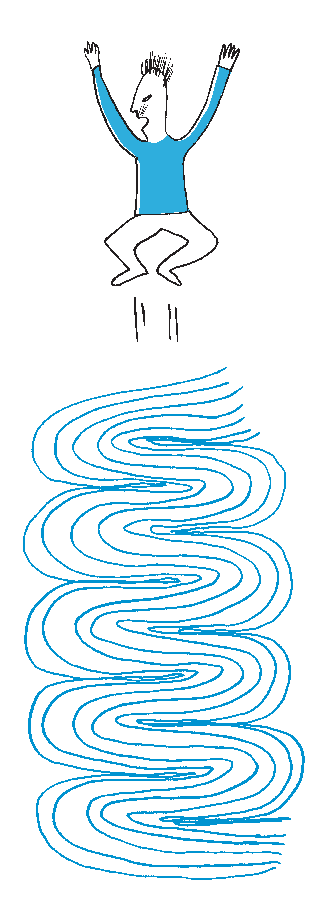
\includegraphics{art/202501_kol09}}
	

\eject



\input 05-tjz

\vfill
\spis{Odwzorowania addytywne i~geometria}
{Franciszek Hansdorfer}

\wtyt{Odwzorowania addytywne i~geometria}

\waut{Franciszek HANSDORFER}

Rozważmy zbiór \marg{Artykuł jest skrótem pracy z~45. edycji
Konkursu Uczniowskich Prac z~Matematyki im. Pawła Domańskiego. Z~pełną jej
wersją można zapoznać się na stronie \href{http://deltami.edu.pl}{\tt deltami.edu.pl}. Autor chciałby bardzo podziękować dr. hab. Mariuszowi Skałbie za opiekę merytoryczną.}
\[K= \{a+b\sqrt{2} : a,b \in \mathbb Q\}.\]

Do tego zbioru należą zatem liczby $1+2\sqrt{2}$ czy
$\frac{2}{3}+\frac{1}{8}\sqrt{2}$. Oczywiście należą do niego wszystkie liczby
wymierne (wystarczy wziąć $b=0$), w~tym liczby $0$ i~$1$. Ponadto jeśli wezmę dowolne dwie
liczby z~$K$, to ich suma i~różnica również należą do $K$. Tak samo jest
z~iloczynem, o~czym przekonuje nas poniższa równość: \begin{equation*}
(a+b\sqrt{2})\cdot (c+d\sqrt{2})= (ac+2bd) + (bc+ad)\sqrt{2}.
\end{equation*}
\marg{\vspace*{0cm}
Strukturę, której elementy możemy dodawać, odejmować, mnożyć i~dzielić
z~wyróżnionymi elementami 0 (którego dodanie nic nie zmienia) i~1 (mnożenie przez które nic nie
zmienia), nazywamy \textit{ciałem}. Ciałem jest zatem zbiór liczb
rzeczywistych, wymiernych, lecz również opisany tu zbiór $K.$
}%
Operacja dzielenia też nie wyprowadza poza $K$, w~czego uzasadnieniu pomaga szkolna sztuczka na
pozbywanie się niewymierności z~mianownika:
\begin{equation*}
\frac{a+b\sqrt{2}}{c+d\sqrt{2}}= 
\frac{(a+b\sqrt{2})(c-d\sqrt{2})}{(c+d\sqrt{2})(c-d\sqrt{2})}= 
\frac{ac-2bd}{c^2-2d^2} + \frac{bc-ad}{c^2-2d^2}\sqrt{2}.
\end{equation*}

Zdefiniujmy teraz funkcję $\sigma: K\to K$ wzorem:
\[\sigma(a+b\sqrt{2}) = a-b\sqrt{2}.\]
\marg{Dla $x\in K$ liczbę $\sigma(x)$ nazywa się często
\textit{sprzężeniem}~$x$.}%
Przekształcenie $\sigma$ w~ten sposób zdefiniowane ma ciekawe własności.
Zacznijmy od tego, że dobrze się ono zachowuje ze względu na dodawanie
i~mnożenie. 
Niech $x=a+b\sqrt{2}$, $y=c+d\sqrt{2}$, gdzie $a,b,c,d\in\mathbb{Q}$. Wtedy:
\begin{equation*}
\begin{split}
\sigma(x+y)&=\sigma(a+c+(b+d)\sqrt{2})=a+c-(b+d)\sqrt{2}\\&=a-b\sqrt{2}
+c-d\sqrt{2}=\sigma{(x)}+\sigma{(y)},\\
\sigma(xy) & =\sigma\left((a+b\sqrt{2})(c+d\sqrt{2})\right)=\sigma(ac+ad\sqrt{2}+bc\sqrt{2} +2bd ) \\& = \sigma\left((ac+2bd)+(ad+bc)\sqrt{2}\right)=(ac+2bd)-(ad+bc)\sqrt{2}\\  & = (a-b\sqrt{2})(c-d\sqrt{2}) = \sigma(x)\sigma(y).
\end{split}
\end{equation*}
Pokazaliśmy, że $\sigma$ jest \textit{addytywna}
i~\marg{\vspace*{0cm}Przedstawione tu własności pozwalają nazwać funkcję
$\sigma$ \textit{automorfizmem} ciała~$K.$}
\textit{multiplikatywna}. Co istotne, zachowuje ona elementy neutralne  dodawania
i~mnożenia, czyli 0 i~1 -- rzeczywiście, $\sigma(0)=0$ oraz $\sigma(1)=1$.

Chociaż $\sigma$ jest bardzo \emph{porządną} funkcją z~algebraicznego punktu
widzenia, to z~analitycznego punktu widzenia już taka regularna nie jest.
Wykażemy mianowicie, że $\sigma$ nie jest
ciągła w~żadnym punkcie.
Przypomnijmy najpierw definicję  Heinego ciągłości funkcji:
\begin{gather*}
\mbox{\emph{$f$ jest ciągła w~punkcie $x_0$ wtedy i~tylko wtedy, gdy:}}
\\
\forall{(x_n)}:\lim_{n\to\infty} x_n =x_0 \implies \lim_{n\to\infty} f(x_n)=f(x_0).
\end{gather*}
Niech więc $x_0 = a+b\sqrt{2}$, gdzie $a,b\in \mathbb Q$.

Definiujemy teraz ciąg $x_n = a+b\sqrt{2}+{(1-\sqrt{2})}^n$. Ponieważ
$|1-\sqrt{2}|<1$, więc
\[\lim_{n\to\infty} x_n = a+b\sqrt{2} = x_0.\]

Korzystając z~własności funkcji $\sigma$, mamy:
\[\sigma(x_n) = \sigma\big(a+b\sqrt{2}+(1-\sqrt{2})^n\big) = a-b\sqrt{2} + (1+\sqrt{2})^n.\vadjust{\eject}\]
Ponieważ $1+\sqrt{2}>1$, więc ciąg $(\sigma(x_n))$ jest rozbieżny. Zatem:
%\[\lim_{n\to\infty} \sigma (x_n) \neq \sigma (x_0).\]
\[ \sigma (x_n) \not\to \sigma (x_0).\]
\marg{
\includegraphics{art/202501_kol12}}Dowiedliśmy więc, że $\sigma$ jest nieciągła w dowolnie
wybranym punkcie $x_0 \in K$.

Spróbujemy teraz zbadać funkcję $\sigma$ pod względem geometrycznym. W~tym celu potrzebujemy odpowiednika funkcji $\sigma$ zdefiniowanego na ,,płaszczyźnie''. Niech więc $F:K^2 \to K^2$ będzie dla $x,y \in K$ określone wzorem:
\[F(x,y) = (\sigma(x), \sigma(y)).\]
Tak zdefiniowane $F$ ma bardzo ciekawe, paradoksalne wręcz, własności.
Z jednej strony $F$ jest bardzo nieregularne, bo wszędzie nieciągłe, co wynika z~wyżej udowodnionej nieciągłości $\sigma$.

Z drugiej jednak strony $F$ jest bardzo regularne, gdyż jest addytywne. Otóż dla $x_1,y_1,x_2,y_2 \in K$ mamy:
\begin{align*}
    F((x_1,y_1) + (x_2,y_2)) & = F(x_1+x_2, y_1+y_2) = (\sigma(x_1+x_2), \sigma(y_1+y_2)) \\&= (\sigma(x_1)+\sigma(x_2), \sigma(y_1)+\sigma(y_2)) = F(x_1,y_1) + F(x_2,y_2).
\end{align*}
Analogicznie możemy uzasadnić, że dla dowolnych $\alpha,x_1,x_2\in K$
zachodzi $F(\alpha\cdot(x_1,x_2))=\sigma(\alpha)\cdot F(x_1,x_2)$.

Co dla nas najważniejsze, z~geometrycznego punktu widzenia $F$
zachowuje pewne podstawowe własności geometryczne.
Po pierwsze, $F$ zachowuje współliniowość punktów. Wynika to
z~faktu, że jeśli $X=(x_1,x_2)$, $Y=(y_1,y_2)$ i~$Z=(z_1,z_2)$ są współliniowymi
punktami z~$K^2$, to $X-Y=\alpha\cdot(X-Z)$ dla pewnej liczby $\alpha\in K$, a~stąd
$F(X)-F(Y)=\sigma(\alpha)\cdot\big(F(X)-F(Z)\big)$. Dlatego obrazami prostych
(w~obcięciu do $K^2$) w~przekształceniu $F$ są proste. Ponieważ jednak funkcja $\sigma$
może zmienić znak lub zamienić liczbę o~module większym od 1 na taką o~module
mniejszym od 1 (np. dla $\alpha=1+\sqrt{2}$), obrazami odcinków nie są odcinki.

Ponadto $F$ zachowuje \textbf{równość odległości}, czyli dla $X,Y,Z,T \in K^2$ mamy:
\begin{equation}
    d(X, Y) = d(Z, T) \implies d(F(X), F(Y)) = d(F(Z), F(T)),
\end{equation}
gdzie przez $d(\cdot ,\cdot)$ oznaczamy euklidesową odległość na
płaszczyźnie.
\marg{\vspace*{-1cm}    {\hspace*{-1.2cm}\begin{tikzpicture}
        \begin{axis}[
                width = 1.2\linewidth,
                height = 1.2\linewidth,
                axis lines=middle,
                ymajorgrids=true,
                xmajorgrids=true,
                xmin=-1.5,
                xmax=5.4,
                ymin=-1.5,
                ymax=5.4,
                xtick={-1,0,...,5},
                ytick={-1,0,...,5},]
            \begin{scriptsize}
                \filldraw[magenta, thick] (1,2.41421) -- (3.41421, 3.41421);
                \filldraw[magenta, thick] (-1,2.41421) -- (0,4.82843);
                \filldraw[black] (1,2.41421) circle (1pt) node[anchor=north east]{$P_1$};
                \filldraw[black] (3.41421, 3.41421) circle (1pt) node[anchor=south west]{$P_2$};
                \filldraw[black] (-1,2.41421) circle (1pt) node[anchor=north]{$Q_1$};
                \filldraw[black] (0,4.82843) circle (1pt) node[anchor=west]{$Q_2$};
                \filldraw[red, thick] (1, -0.414214) -- (0.585786, 0.585786);
                \filldraw[red, thick] (0, 0.585786) -- (1, 0.171573);
                \filldraw[black] (1, -0.4142141) circle (1pt) node[anchor=north]{$F(P_1)$};
                \filldraw[black] (0.585786, 0.585786) circle (1pt) node[anchor=south]{$F(P_2)$};
                \filldraw[black] (0, 0.585786) circle (1pt) node[anchor= east]{$F(Q_1)$};
                \filldraw[black] (1, 0.171573) circle (1pt) node[anchor= west]{$F(Q_2)$};
            \end{scriptsize}
        \end{axis}
    \end{tikzpicture}}\\[4pt]
		Rys. 1 
    }
Sprawdzenie jest proste. Niech $X = (x_1, x_2), Y= (y_1, y_2), Z=(z_1,z_2), T=(t_1,t_2)$. Ponieważ
$d((x_1,x_2), (y_1, y_2)) = d((z_1, z_2), (t_1, t_2))$, więc
\[(y_1-x_1)^2 + (y_2-x_2)^2 =(t_1-z_1)^2 + (t_2 - z_2)^2.\]
Do obu stron przykładamy funkcję $\sigma$:
\[(\sigma(y_1) -\sigma(x_1))^2 +(\sigma(y_2) - \sigma(x_2))^2 = (\sigma(t_1) - \sigma(z_1))^2 + (\sigma(t_2) - \sigma(z_2))^2 .\]
Zatem
\[d(F(X), F(Y)) = d(F(Z), F(T)).\]

To, że $F$ zachowuje równość odległości, nie oznacza jednak, że jest izometrią.
Na przykład dla punktów $P_1 = (1,1+\sqrt{2}), P_2 = (2 + \sqrt{2}, 2 +
\sqrt{2}),$ ${Q_1 = (-1,1+\sqrt{2}), Q_2 = (0,2+2\sqrt{2})}$ mamy
$d(P_1,P_2) = d(Q_1, Q_2)$. Ale na mocy~(1) mamy też $d(F(P_1), F(P_2)) =
d(F(Q_1), F(Q_2))$, jednakże, jak można zobaczyć na rysunku 1 (lub obliczyć),
$d(P_1,P_2) \neq d(F(P_1), F(P_2))$.

\marg{\vspace*{-.8cm}
\hspace*{-.8cm}\begin{tikzpicture}%[scale=.85]
        \begin{axis}[
                width = 1.2\linewidth,
                height = 1.2\linewidth,
                axis lines=middle,
                ymajorgrids=true,
                xmajorgrids=true,
                xmin=-1.4,
                xmax=5.4,
                ymin=-1.4,
                ymax=5.4,
                xtick={-2,-1,0,...,5},
                ytick={-1,0,...,5},]
            \begin{scriptsize}
                \filldraw[color=black, fill=magenta,fill opacity=0.3, thick] (1.70711, 4.41421) -- (2.41421, 1.70711) --(3.70711, 1.70711)-- cycle;
                \filldraw[black] (1.70711, 4.41421) circle (1.5pt) node[anchor=east]{$P_1$};
                \filldraw[black] (2.41421, 1.70711) circle (1.5pt) node[anchor=north]{$P_2$};
                \filldraw[black] (3.70711, 1.70711) circle (1.5pt) node[anchor=north west]{$P_3$};
                \filldraw[color=black, fill=magenta,fill opacity=0.3, thick] (0.292893, 1.58579) -- (-0.414214, 0.292893) -- (2.29289, 0.292893) -- cycle;
                \filldraw[black] (0.292893, 1.58579) circle (1.5pt) node[anchor=south]{$F(P_1)$};
                \filldraw[black] (-0.414214, 0.292893) circle (1.5pt) node[anchor=east]{};%$F(P_2)$};
                \filldraw[black] (2.29289, 0.292893) circle (1.5pt) node[anchor=west]{$F(P_3)$};
            \end{scriptsize}
        \end{axis}
      \end{tikzpicture}\raise31.5pt\llap{$F(P_{2})$\kern94pt}\\[4pt]
		Rys. 2. Przekształcenie $F$ może zamienić
		wierzchołki trójkąta ostrokątnego na
		rozwartokątnego. Na powyższym rysunku mamy $P_1 = (1+\frac{\sqrt{2}}{2},3+\sqrt{2}),
P_2 = (1+\sqrt{2},1+\frac{\sqrt{2}}{2}), P_3 =
(3+\frac{\sqrt{2}}{2},1+\frac{\sqrt{2}}{2})$
		}
		Poza tym $F$ zachowuje prostopadłość wektorów. Niech $X, Y, Z \in K^2$
		i~załóżmy, że $\angle YXZ=90^\circ$, czyli $\langle X-Y, X-Z\rangle =0$:
\[( x_1-y_1 )( x_1-z_1 ) + ( x_2-y_2 )( x_2-z_2 ) = 0.\]
Po przyłożeniu funkcji $\sigma$ do obu stron otrzymujemy:
\[\big( \sigma(x_1)-\sigma(y_1) \big)\big( \sigma(x_1)-\sigma(z_1) \big) + \big(
\sigma(x_2)-\sigma(y_2) \big)\big( \sigma(x_2)-\sigma(z_2) \big) =
\sigma(0)=0,\]
czyli
\[\angle F(Y)F(X)F(Z) = 90^\circ.\]

		W ogólności przekształcenie $F$ nie zachowuje jednak kątów między
		prostymi, co ilustruje rysunek~2.

Przekształcenie $F$ godzi w~sobie sprzeczne natury: \emph{dziką} naturę
analityczną (nigdzie nie jest ciągłe) i~\emph{łagodną} naturę
algebraiczno-geometryczną (jest addytywne, zachowuje równość odległości
i~prostopadłość wektorów).  Zachęcam Czytelnika do własnych badań nad jego
własnościami!




%
\tjzspis{Człowiek ukryty w genomie} %tytuł do spisu treści
\tjztyt{Człowiek ukryty w genomie} %tytuł odcinka 


{%\advance\baselineskip by-.1pt\advance\parskip by-1pt
W połowie lutego 2001 roku amerykański noblista, mikrobiolog, David Baltimore we wstępniaku do magazynu Nature wyznał: ,,Widziałem wiele ekscytujących odkryć z biologii w ciągu ostatnich 40 lat, jednak czułem ciarki na plecach, gdy czytałem artykuł opisujący zarys naszego genomu''. 

Zapowiadał w ten sposób pracę, w której konsorcjum Human Genome Project opisywało wstępne wyniki sekwencjonowania ludzkiego DNA. Start projektu w 1990 roku ogłosił sam James Watson, który porównał zadanie rozszyfrowania informacji ukrytej w ludzkim DNA do misji lądowania człowieka na Księżycu. 

Przez kilkanaście lat napięcie rosło, oczekiwania były olbrzymie, miało się przecież okazać, jak na poziomie cząsteczek realizowane jest powstanie człowieka. Jednym z ważniejszych parametrów, o którym dyskutowano, była liczba genów
% sprawiających, że jesteśmy ludźmi.
zakodowanych w~naszym DNA.
Wiadomo było już sporo o liczbie genów u innych organizmów.  np. bakteria \textit{Escherichia coli} ma ich około 4 tysięcy, maleńka roślina, rzodkiewnik pospolity -- 25,5 tysiąca, a mierzący 1 mm nicień \textit{Caenorhabditis elegans} około 20 tysięcy. 

Dziś mogę fantazjować, że może tuż po ciarkach u noblisty pojawiły się  krople potu, bowiem wstępny wynik był zadziwiający: ogłoszono, że genom ludzki koduje między 20 tysięcy a 30 tysięcy genów. Ta  skromna liczba mogła podsuwać wątpliwości, czy w opisie funkcjonowania żywych komórek nie popełniono fundamentalnego błędu?

Tu muszę doprecyzować, co w tej wyliczance oznacza słowo ,,gen''. Definiowano go jako fragment DNA, w którym zakodowana jest informacja o budowie białka. Białko zaś to cząsteczka, która się składa z łańcucha nie mniej niż 100 aminokwasów. 

Analiza całego genomu ludzkiego wykazała, że sekwencje, które kodują białka, to jedynie 1 do 2\% całości. Powstało zatem pytanie: co znajduje się w pozostałej ,,ciemnej materii'' (\textit{dark genome})?

Po ponad 20 latach wiemy  więcej, choć wiele pozostaje do wyjaśnienia. 

Najwięcej jest reliktów z przeszłości, fragmentów samorzutnie kopiujących się, pradawnych wirusów i innych aktywnych elementów, które są skutkiem procesów zachodzących w DNA. Dużą część genomu stanowią sekwencje kodujące różne typy RNA, cząsteczek, które mają fundamentalne funkcje dla życia komórki. Biorą udział w tworzeniu struktur niezbędnych do produkcji białek. Wiele z nich, w tym bardzo krótkie, reguluje działanie genów: ilość produkowanych białek, to, jak długo są produkowane i jak szybko są degradowane. Nie można też zapomnieć o fragmentach pełniących funkcje strukturalne -- dzięki niektórym bardzo długie cząsteczki DNA mogą być pakowane do struktur odpornych na uszkodzenia mechaniczne, co jest krytyczne w trakcie podziałów komórkowych; inne sprawiają, że cząsteczki DNA nie ulegają skracaniu; a dzięki innym DNA może być duplikowany.  

Czas eksploracji jeszcze się nie skończył. John Prensner, neuroonkolog dziecięcy z~Bostonu po bezskutecznych,
% postanowił sprawdzić, co ukrywa się w zakamarkach genomu, ponieważ prowadzone przez niego
poszukiwaniach genów związanych z nowotworami u dzieci
wrócił do analizy genomu, zmieniając kryteria wyszukiwania.
% okazywały się bezskuteczne.
Podstawą były
sporadyczne
% pojawiające się od jakiegoś czasu
informacje o istnieniu w komórkach cząsteczek będących łańcuchami aminokwasów krótszych niż 100. Prensner przyznaje, że było mu trudno uzyskać finasowanie dla badań nad takimi minibiałkami, gdyż uznawano je dotąd za komórkowe ,,śmieci'', szybko ulegające degradacji. Udało mu się jednak zgromadzić międzynarodowe grono, które podjęło się poszukiwania minibiałek. Dzięki analizie wielu prac badawczych i baz danych kanoniczna definicja ,,białko to więcej niż 100 aminokwasów'' została w końcu podważona. 

Okazało się, że spośród 7264 sekwencji, które mogłyby kodować minibiałka, około jedna czwarta  jest aktywna, dzięki czemu powstaje około 3000~różnych minibiałek (jedna sekwencja DNA może kodować więcej niż jedno~białko). \marg{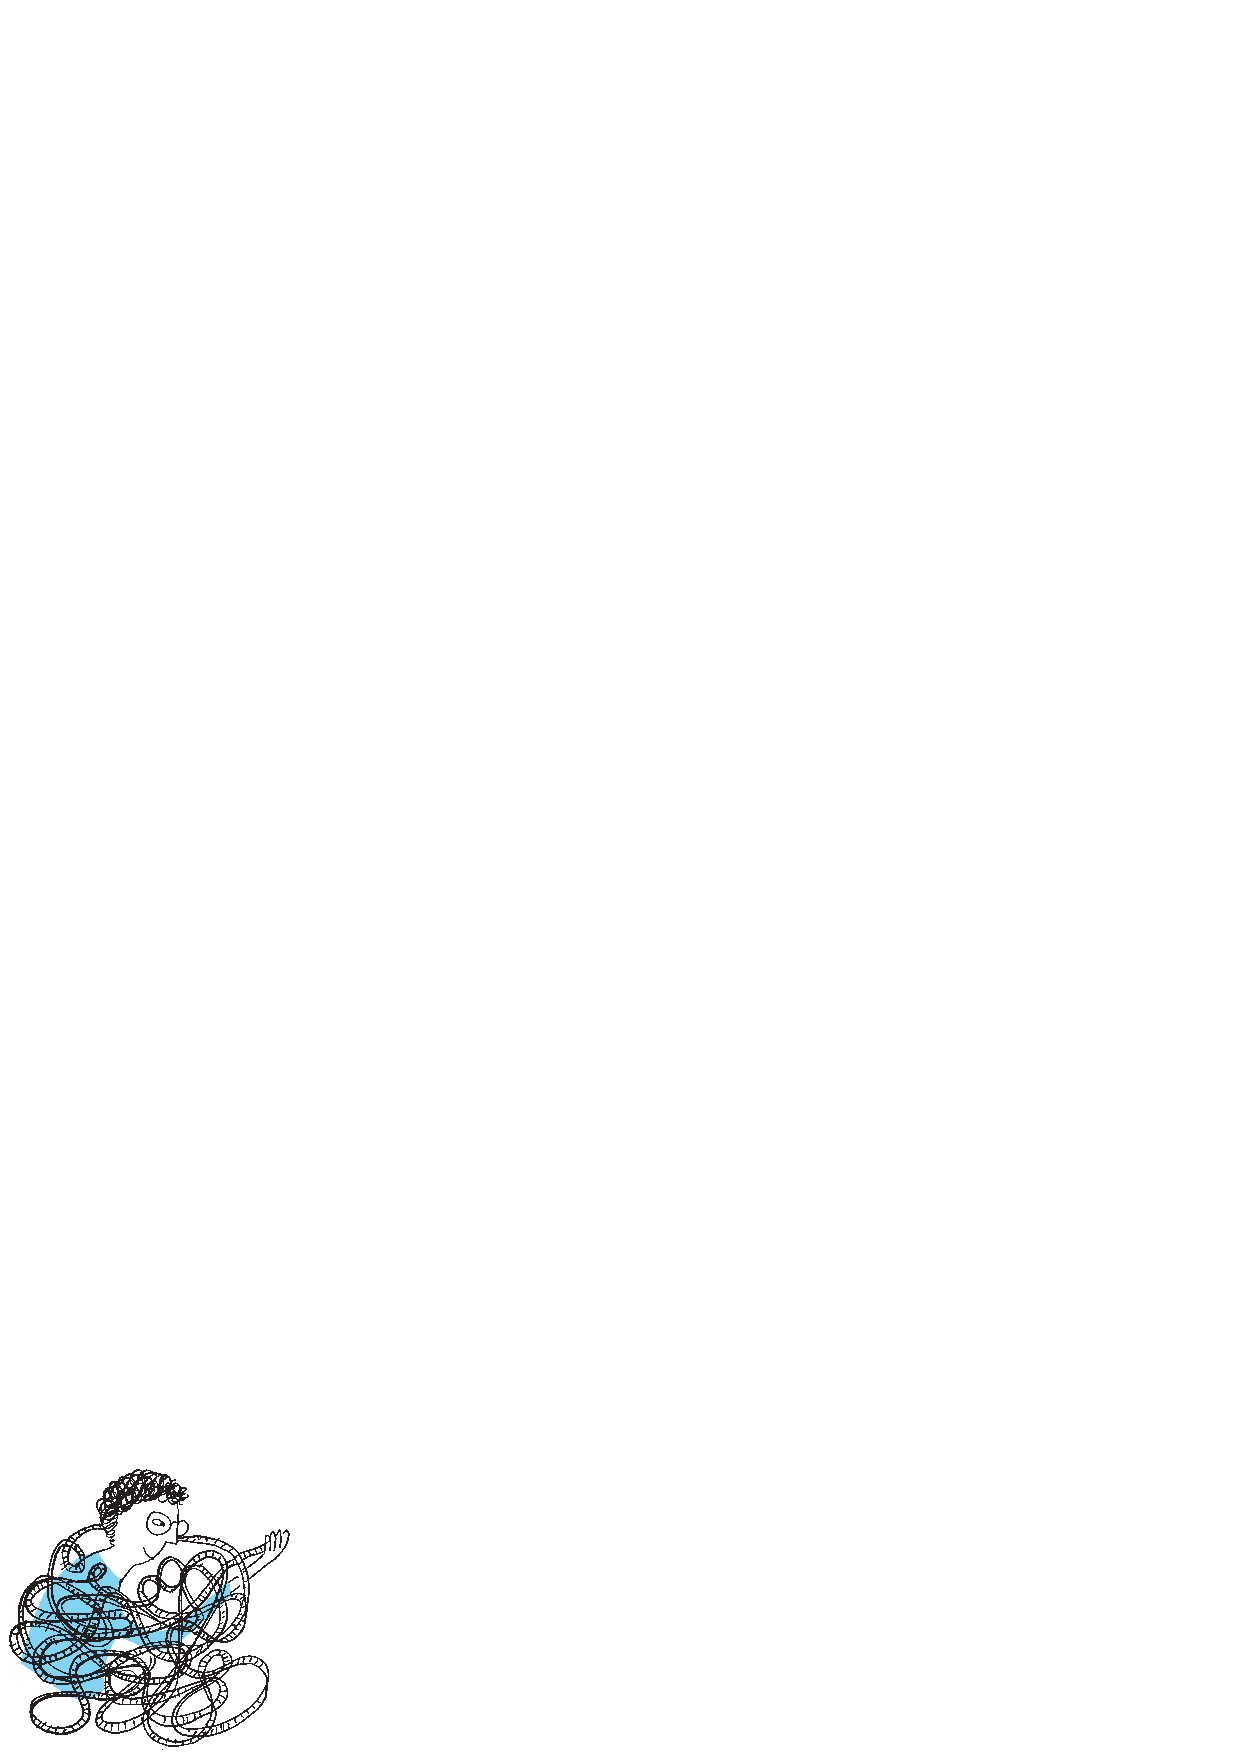
\includegraphics{art/202501_kol10}}

Jedno z nich, ASDURF, jest na przykład produkowane w nadmiarze w komórkach rdzeniaka zarodkowego, trudnego do zdiagnozowania nowotworu dziecięcego. Jego nadprodukcja wydłuża czas życia komórek nowotworowych. Inne badania wskazują na rolę mikrobiałek w rozwoju otyłości, raka trzustki i w chorobach metabolicznych.

Co zatem stanowi esencję ,,człowieka'' na poziomie cząsteczek? Jako jedyny gatunek, który jest w stanie analizować własny genom, musimy wciąż zachować pokorę dla złożoności rozwiązań natury i cierpliwie szukać dalszych odpowiedzi. Bo przecież wiadomo było, że to nie może być proste{\dots}


}

\medskip
\rightline{\large\it Marta FIKUS-KRYŃSKA}

\hspace*{-5.5cm}\vrule height5pt depth-4.5pt width18cm

\normalsize

\endinput
\marg{Kiedyś uważano, że za każdą cechę odpowiada jeden gen. Czyli jest np. gen jasnych włosów, brązowych włosów, czarnych włosów, jest gen dobrego węchu czy też dobrego wzroku itp. Dziś wiemy, że tak zwanych cech jednogenowych jest bardzo, bardzo niewiele, a większość z naszych cech determinuje kilkaset genów!}


\makeatletter
\def\@oddhead{\hfill}
\def\@evenhead{\hfill}
\makeatother

\normalsize
\aktspis{}
\akthead
%\begin{dwieszpalty}
\mtyt{}

%\advance\baselineskip by-.1pt%\vspace*{\parskip}
% \begin{dwieszpalty}
%\medskip
%\vskip\parskip

\rightline{\large \it  Krzysztof TURZYŃSKI}
%\end{dwieszpalty}


%\end{dwieszpalty}

\normalsize
\setcounter{equation}0
\newcommand{\red}[1]{#1}
\newcommand{\add}[1]{#1}
\newcommand{\nnote}[1]{}
\newcommand{\note}[1]{}
\newcommand{\uunit}[1]{[#1]}

\newcommand{\ddlink}[3]{\href{#1}{$\Delta^{#2}\sb{#3}$}}
\spis{Trzecie prawo Keplera i~analiza wymiarowa}
{Grzegorz Łukaszewicz}

\wtyt{Trzecie prawo Keplera\\ i~analiza~wymiarowa}

\waut{Grzegorz ŁUKASZEWICZ*}
\aafil{Wydział Matematyki, Informatyki i~Mechaniki, Uniwersytet Warszawski}


{\it Drogi, którymi ludzie dochodzą do poznania niebios, wydają mi się nie mniej godne podziwu niż same niebiosa.}

\rightline{(Johannes Kepler)}

\advance\baselineskip by.2pt
\marg{

\includegraphics[width=0.3\textwidth]
{220px-Johannes_Kepler_1610} \\[4pt]
Johannes Kepler (1571--1630)
\bigskip


Najogólniejsza forma trzeciego prawa Keplera wyraża się wzorem $r_{\rm mean}^3 \varpropto T^2$ ($\varpropto$ -- ,,proporcjonalne do''), gdzie $T$ jest czasem obiegu planety po orbicie eliptycznej, a~$r_{\rm mean}$~jest ,,średnią odległością'' planety od Słońca.


\bigskip
Kepler obsesyjnie poszukiwał pitagorejskich harmonii w~Układzie Słonecznym. Tak pisze o~odkryciu swojego trzeciego prawa w~1618 roku: \\[1mm]
{\it Lecz teraz, odkąd osiemnaście miesięcy temu [zajaśniało] pierwsze światło, trzy miesiące temu jasny dzień, a~kilka dni temu rozbłysło pełnym blaskiem słońce mych cudownych spekulacji -- nic mnie już nie powstrzyma. Oddaję się swobodnie świętemu szaleństwu.} ,,Harmonices Mundi'', wg Jerzy Kierul: ,,Kepler'', PIW, 2007.


}%
Celem tego artykułu jest przybliżenie Czytelnikowi problemów związanych ze sformułowaniem przez Keplera jego trzeciego prawa, \emph{wiążącego czas obiegu planety po orbicie eliptycznej z~parametrami opisującymi jej wymiary}, oraz pokazanie, jak analiza wymiarowa, która wyrosła z~próby rozszerzenia na fizykę greckich koncepcji podobieństwa geometrycznego, stosunku i~proporcji, może pomóc w~\emph{odkryciu tego prawa fizycznego} w~jego współczesnym sformułowaniu. Na koniec rozważymy główne założenia metody analizy wymiarowej, jej podstawy metafizyczne oraz zalety i~ograniczenia. 


Postawmy się w~sytuacji, w~której niewiele wiemy i~poszukujemy powyższego związku w~postaci równania algebraicznego postaci $f(T_o, r_{\rm mean})= \mathrm{const}$, gdzie $T_o$ oznacza czas obiegu planety po elipsie, natomiast $r_{\rm mean}$ oznacza jedną ze średnich odległości planety od Słońca, np. średnią arytmetyczną czy średnią geometryczną z~obu półosi, $a$, $b,$ elipsy lub jeszcze inną ,,średnią odległość''. 

  
Postępując ścieżką metody {\it analizy wymiarowej},  
musimy najpierw dociec, jakie wielkości są ważne w~naszym zagadnieniu. Rozsądnym jest przyjęcie, że ważnymi parametrami są czas obiegu planety po elipsie $T_o$, wymiary półosi elipsy $a$, $b$, masa planety $m$, masa Słońca $M_s$ oraz stała grawitacji $G$. Ruch odbywa się w~centralnym polu grawitacyjnym, 
$\vec{F} = -G\frac{M_s m}{r^2}\frac{\vec{r}}{r}$.
 
Oznaczmy przez $\uunit{X}$ jednostkę, w~jakiej mierzymy wielkość $X$. 
Mamy
\begin{eqnarray}\label{jednostki1}
 \uunit{a}=L, \ \uunit{b}=L, \ \uunit{m}=M, \ \uunit{M_s}=M, \ 
\uunit{T_o}=T, \ \uunit{G}=\frac{L^3}{MT^2},
\end{eqnarray}
gdzie $L$, $M$, $T$ są pewnymi jednostkami 
{\it wielkości fundamentalnych}: długości, masy i~czasu, w~mechanice Newtona. Tutaj stała grawitacji $G$ jest {\it wielkością pochodną}, mierzoną w~jednostce będącej kombinacją potęg jednostek wielkości fundamentalnych.
Rozwiązanie naszego problemu powinno być zawarte w~relacji postaci 
\begin{eqnarray}\label{formuła1}
 f(a, b, m, M_s, T_o, G)=0,
\end{eqnarray}
w~której zmiennymi są liczby dodatnie wyrażające długość, masę, czas i~stałą grawitacji, mierzone w~jednostkach danych w~\eqref{jednostki1}.

Załóżmy, że powyższa relacja jest \emph{niezmiennicza} ze względu na zmianę jednostek, z~$L,M,T$ na jednostki $L',M',T'$ postaci 
$L'=\alpha L, M'=\beta M, T'=\gamma T$, gdzie 
$\alpha, \beta, \gamma$ są dowolnymi liczbami dodatnimi. Oznacza to, że w~jednostkach $L',M',T'$ relacja \eqref{formuła1} ma tę samą postać 
$f(a',b',m',M_s', T_o', G')=0$. Mamy zatem
\begin{eqnarray}
%  f(a, b, m, M_s, T_o, G)=
 f \left(\frac{a}{\alpha},\frac{b}{\alpha},\frac{m}{\beta},
 \frac{M_s}{\beta},\frac{T_o}{\gamma},\frac{G\gamma^2\beta}{\alpha^3}\right)=0.
\end{eqnarray}
Wybierając $\alpha=a$, $\beta=M_s$, $\gamma=T_o$ i~oznaczając
\[
\Pi_1=\frac{b}{a}, \quad 
\Pi_2=\frac{m}{M_s}, \quad 
\Pi_3=\frac{GM_sT_o^2}{a^3},
\]
otrzymujemy
\begin{eqnarray}\label{rel}
f(1,\Pi_1,\Pi_2, 1,1,\Pi_3) =
f \left(1, \frac{b}{a}, \frac{m}{M_s},1,1,\frac{GM_sT_o^{2}}{a^3}\right)
= 0,
\end{eqnarray}
gdzie teraz $\Pi_1,\Pi_2,\Pi_3$ są wielkościami {\it bezwymiarowymi}.
\add{Przyjmijmy, że równanie~\eqref{rel} można rozwiązać ze względu na $\Pi_3$, czyli wyrazić tę zmienną poprzez dwie pozostałe przy użyciu pewnej funkcji $\psi$:}
\begin{equation}\label{invariance1}
   \frac{GM_sT_o^2}{a^3} = \psi(\Pi_1,\Pi_2)=
   \psi\left(\frac{b}{a},\frac{m}{M_s}\right).
\vadjust{\eject}\end{equation}
\begin{dwieszpalty}\looseness-1 {\spaceskip.33em minus.08emMając do dyspozycji  wzór \eqref{invariance1}, Kepler wiedziałby, że jest na dobrym tropie. Natychmiast zauważyłby, że ponieważ orbity eliptyczne wszystkich znanych mu planet Układu Słonecznego są zbliżone do okręgów, a~masy planet są zaniedbywalne w~porównaniu z~masą Słońca, więc prawe strony wzoru dla poszczególnych planet powinny być liczbami niewiele oscylującymi wokół wartości $\psi(1,0)$. Warto przypomnieć, że Mikołaj Kopernik, idąc za tradycją starożytnych, traktował orbity planet jako okręgi. Nie mógłby zresztą odkryć elipsy, ponieważ nie dysponował wystarczająco dokładnymi obserwacjami. Kepler miał już dokładniejsze dane, oparte na obserwacjach Tychona Brahego. W~obliczeniach prowadzących do {\it oryginalnego keplerowskiego sformułowania trzeciego prawa, z~%
jedną stałą dla wszystkich planet}, Merkury sprawiał mu kłopot ze względu na swój mimośród, który jest od jednego do dwóch rzędów większy niż mimośrody innych znanych wtedy planet. Kepler wykluczył więc go z~rozważań. Czy dobrze zrobił?}


Okazało się, że nie, ale Kepler nie mógł jeszcze skorzystać z~mechaniki Newtona,  powstała dopiero później. Jej konsekwencją jest piękny wzór:\vspace*{2pt}
\begin{equation}\label{piękny}
   \frac{GM_sT_o^2}{r_{\mathrm{mean}}^3} =
  \frac{4\pi^2}
  {(1+\frac{m}{M_s})(1-e^2)^{\frac{3}{4}}}\,,\vspace*{2pt}
\end{equation}
będący Newtonowską wersją trzeciego prawa Keplera.
 Przypatrzmy mu się dokładniej. Zawiera on jawnie wszystkie istotne dla astronomów parametry dynamiczne i~geometryczne: stałą grawitacji $G$, masę Słońca $M_s$, czas obiegu planety po orbicie $T_o$ i~jedną z~naturalnych średnich z~obu półosi planety, średnią geometryczną $r_{\mathrm{mean}}=\sqrt{ab}$, określającą średnią odległość planety od Słońca -- po lewej stronie równania oraz
stosunek masy planety do masy Słońca $\frac{m}{M_s}$ i~mimośród planety $e=\sqrt{1-(\frac{b}{a})^2}$ określający jej kształt -- po prawej stronie równania.

W przypadku, gdy masy planet są zaniedbywalne w~porównaniu z~masą Słońca, a~ich mimośrody są bardzo małe, to w~granicy 
$\frac{m}{M_s}\to 0$, $e\to 0$ prawa strona jest wtedy równa $4\pi^2$, czyli z~dokładnością do czterech miejsc po przecinku $39{,}4784$.  

Sprawdźmy teorię Newtona. W~tym celu należy popatrzeć w~niebo i~mierzyć. Napięcie rośnie, gdyż jej niezgodność z~trzecim prawem Keplera, które dość dokładnie zgadza się z~obserwacjami astronomicznymi,  
zaprzeczałaby jej uniwersalności.
Mamy następujące dane astronomiczne
(za średni promień orbity przyjmujemy tu $r_{\mathrm{mean}} = \sqrt{ab}$):

\vskip2\parskip

% \begin{table}[h!]
%    \centering
 \centerline{\footnotesize\tabcolsep3pt\def\arraystretch{1.2}\def\ccc #1 {\multicolumn{1}{c|}{#1}}\begin{tabular}{|l|r@{~~\,}|r@{\ \qquad}|r@{\quad}|c|}
   \hline
   Ciało &\ccc Okres &\ccc Średni &\ccc Wielokrotność & Mimośród\vrule height10pt width0pt\\[-3pt]
   niebieskie &\ccc obiegu &\ccc promień~orbity &\ccc masy & orbity \\[-2pt]
   &\ccc w~latach &\ccc w~${\rm km\times 10^{-6}}$ &\ccc Ziemi & \\
   \hline
%   Słońce\vrule height10pt width0pt &\ccc --- &\ccc --- & $332\,488{,}0\phantom{000}$ & --- \\
%   Merkury & $0{,}241$ & $57{,}9$ & $0{,}0543$ & $0{,}2056$ \\
%   Wenus & $0{,}615$ & $108{,}1$ & $0{,}8136$ & $0{,}0068$ \\
%   Ziemia & $1{,}000$ & $149{,}5$ & $1{,}0000$ & $0{,}0167$ \\
%   Mars & $1{,}881$ & $227{,}8$ & $0{,}1069$ & $0{,}0934$ \\
%   Jowisz & $11{,}862$ & $777{,}8$ & $318{,}35\phantom{00}$ & $0{,}0484$ \\
%   Saturn & $29{,}458$ & $1426{,}1$ & $95{,}3\phantom{000}$ & $0{,}0557$ \\
%   Uran & $84{,}015$ & $2869{,}1$ & $14{,}58\phantom{00}$ & $0{,}0472$ \\
%   Neptun & $164{,}788$ & $4495{,}6$ & $17{,}26\phantom{00}$ & $0{,}0086$ \\
%Pluton & $247{,}697$ & $5898{,}9$ & $<0{,}1\phantom{000}$ & $0{,}2485$ \\
Słońce & --- & --- & $332\,488{,}0\phantom{000}$ & --- \\
   Merkury & $0{,}241$ & $57{,}3$ & $0{,}0543$ & $0{,}2056$ \\
   Wenus & $0{,}615$ & $108{,}2$ & $0{,}8136$ & $0{,}0068$ \\
   Ziemia & $1{,}000$ & $149{,}6$ & $1{,}0000$ & $0{,}0167$ \\
   Mars & $1{,}881$ & $227{,}4$ & $0{,}1069$ & $0{,}0934$ \\
   Jowisz & $11{,}863$ & $777{,}9$ & $318{,}35\phantom{00}$ & $0{,}0484$ \\
   Saturn & $29{,}447$ & $1425{,}7$ & $95{,}3\phantom{000}$ & $0{,}0539$ \\
   Uran & $84{,}017$ & $2869{,}0$ & $14{,}58\phantom{00}$ & $0{,}0473$ \\
   Neptun & $164{,}791$ & $4498{,}3$ & $17{,}26\phantom{00}$ & $0{,}0086$ \\
   Pluton & $248{,}021$ & $5812{,}8$ & $<0{,}1\phantom{000}$ & $0{,}2488$ \\
   \hline
   \end{tabular}}
%    \caption{Planety i ich orbity}
% \end{table}

% \includegraphics[width=0.8\textwidth]
% {Kepler3_table.png} 
%  Planety i ich orbity. 


\vskip\parskip

Stąd otrzymujemy interesujący nas diagram pokazujący wartości $\frac{GM_s T_o^2}{r_\mathrm{mean}^3}$ dla kolejnych ciał Układu Słonecznego.

\vskip2\parskip
\centerline{\begin{tikzpicture}[scale=.8]
    \begin{axis}[
        % title={Planetary Data},
        xlabel={},
        % xlabel={Ciała niebieskie},
        % ylabel={$\frac{GM_sT_o^2}{a^3}$},
        % ylabel style={rotate=-90, at={(0.02,0.7)}},
        xtick={1,2,3,4,5,6,7,8,9},
        xticklabels={},
        ytick={3.90, 3.95, 4.00, 4.05, 4.10, 4.15},
        yticklabels={39{,}0, 39{,}5, 40{,}0, 40{,}5, 41{,}0, 41{,}5},
        ymin=3.90, ymax=4.15,
        grid=both,
        width=12cm,
        height=8cm
    ]
    \addplot[
        only marks,
        mark=*,
        mark size=2pt
    ] coordinates {
    (1, 4.077850621616459)
    (2, 3.947906419282189)
    (3, 3.948621433096381)
    (4, 3.9735822373369696)
    (5, 3.95122428727248)
    (6, 3.955054303634854)
    (7, 3.9504572394466804)
    (8, 3.9431207878373344)
    (9, 4.139402324061695)
    };
    \pgfplotsextra{
        \foreach \x/\y/\label in {2/3.9479/Wenus, 3/3.9486/Ziemia, 4/3.9736/Mars, 5/3.9512/Jowisz, 6/3.9551/Saturn, 7/3.9505/Uran, 8/3.9431/Neptun} {
            \node[anchor=west, rotate=90] at (axis cs:\x, \y+0.001) {\label};
        }
        \foreach \x/\y/\label in {1/4.0779/Merkury, 9/4.1394/Pluton} {
            \node[anchor=east, rotate=90] at (axis cs:\x, \y-0.001) {\label};
        }
    }
    \end{axis}
\end{tikzpicture}}
 
Przyglądając się powyższemu diagramowi, widzimy, że przeprowadzone obliczenia rzeczywiście potwierdzają teorię Newtona. Większe odchylenia dla Merkurego
i~Plutona od stałej granicznej $4\pi^2$ wynikają z ich dużych mimośrodów.

Możemy teraz powrócić do wzoru (\ref{invariance1}). Dokonując prostego rachunku na wzorze (\ref{piękny}), możemy napisać wzór (\ref{invariance1}) w~ostatecznej formie jako\vspace*{2pt}
\begin{equation}\label{invariance3}
   \frac{GM_sT_o^2}{a^3} =
  \frac{4\pi^2}
  {1+\frac{m}{M_s}}.\vspace*{2pt}
\end{equation} 
Wzory (\ref{piękny}) i~(\ref{invariance3}) są równoważne i~oba reprezentują trzecie prawo Keplera. Ze wzorów (\ref{invariance1}) i~(\ref{invariance3}) wynika, że stała $\psi(1,0)$ jest równa $4\pi^2$. 
\end{dwieszpalty}

{\scriptsize
\hspace*{-5.5cm}\begin{tabular}{@{}l@{\qquad}l}
\includegraphics[width=0.45\textwidth]
{harm-poly-photo-1} 
\includegraphics[width=0.45\textwidth]{harm-poly-photo-2}&

\includegraphics[width=0.45\textwidth]{Harm-mus-photo2} \\[8pt]
Pomysły \add{Keplera} z~wielościanami&Układ planet i~harmonie w~muzyce
                \end{tabular}
                }\eject

Gwoli ścisłości historycznej należy powiedzieć, że nie ma pewności co do tego, jak Kepler rozumiał swoje trzecie prawo,
\marg{
Prowadzone są dyskusje, jak rozszyfrować oryginalne sformułowanie   trzeciego prawa Keplera. \\[1mm]
{\it Jest jednak całkowicie pewne i~dokładne, że stosunek czasów okresowych dowolnych dwóch planet jest dokładnie stosunkiem potęgi 3/2 średnich odległości, to jest samych kul; pod warunkiem jednak, że średnia arytmetyczna obu średnic orbity eliptycznej będzie nieco mniejsza niż dłuższa średnica.} ,,Harmonices Mundi''
}
gdyż w~,,Harmonices Mundi'' nie określa on w~jasny sposób, co rozumie przez ,,średnią odległość'', a~zgodność jego oryginalnego trzeciego prawa z~{jego} pomiarami orbitalnymi ruchu planet dotyczyła tylko orbit o~bardzo małych mimośrodach. Jak wspomnieliśmy, Merkury sprawiał mu kłopot, podobnie jak później wielu innym [Dembny,~2023]. Oryginalne sformułowanie Keplera nie mogło być sformułowaniem~(\ref{invariance3}), gdyż nie występuje w~nim mimośród, natomiast w~zasadzie  mogło być  sformułowaniem~(\ref{piękny}). %W~artykule nie wyklucza ono Merkurego.
W~artykule [Vijaya, 2019] można znaleźć wnikliwą rekonstrukcję rozumowania Keplera, prowadzącą do propozycji oryginalnej keplerowskiej ,,średniej odległości''.
\normalsize
  
Oczywiście Kepler nie wiedział jeszcze nic o~Uranie i~Plutonie. (Pluton został wykreślony z~listy planet przez
% wykluczony z~układu planet przez
Międzynarodową Unię Astronomiczną, IAU, 
bez zgodnego poparcia społeczności, nie tylko astronomów, w~2006 roku).\marg[-25]{
Średnia odległość planety od Słońca względem zmiennej $p$ wyraża się poprzez całkę
\[
r_p=\frac{1}{p}\int r(p)dp, 
\]
gdzie $r$ jest promieniem wodzącym planety po orbicie eliptycznej. Na~przykład średnie mierzone względem czasu ($t$), długości łuku ($s$) i~kąta obrotu ($\theta$) dla ruchu po okręgu z~centrum pola sił w~jego centrum są równe sobie (równe promieniowi okręgu), natomiast dla elipsy o~półosiach $a$, $b$ różnią się od siebie, \\
$r_t = a(1+e^2/2)$, $r_s=a$, $r_{\theta}=b$,
[Stein, 1977].
}

%%%%%%%%%
%https://www.astronomy.com/science/is-pluto-a-planet-%the-experts-break-it-down/
%%%%%%%%%

{\bf Krótkie podsumowanie metody analizy wymiarowej.} W~rozważanym powyżej zagadnieniu najpierw wyodrębniliśmy {\it istotne} dla jego rozwiązania wielkości fizyczne. Następnie {\it przyjęliśmy} długość, masę i~czas jako wielkości fundamentalne, a~stałą grawitacji jako wielkość pochodną, dającą się przedstawić jako iloczyn potęg wielkości fundamentalnych. Dalej {\it postulowaliśmy} istnienie pewnej relacji między istotnymi wielkościami, {\it niezmienniczej} ze względu na skalowanie. Korzystając z~niezmienniczości tej relacji, otrzymaliśmy, poprzez odpowiednie skalowanie, relację wiążącą ze sobą trzy bezwymiarowe wielkości.
Relacja ta zawierała w~sobie trzecie prawo Keplera.
{\it Matematyczne uzasadnienie} przeprowadzonych operacji jest zawarte w~najważniejszym twierdzeniu metody analizy wymiarowej, tzw. {\bf Twierdzeniu $\Pi$}, [Barenblatt, 2003], [Birkhoff, 1960], [Cantwell, 2002].

Powyższy przykład pokazuje zarówno siłę, jak i~pewne ograniczenia analizy wymiarowej.
O~sile tej metody świadczy to, że przy jej pomocy wyprowadziliśmy trzecie prawo Keplera, niewiele wiedząc o~fizyce zagadnienia. Metoda ta pozwala znaleźć prawidłową odpowiedź w~rozmaitych sytuacjach, gdy nie mamy wielu danych. Potrzebna jest natomiast świadomość pozwalająca założyć czy zgadnąć, od jakich wielkości ta odpowiedź może zależeć.
Zauważmy, że gdybyśmy w~definicji $\Pi_3$ użyli masy planety, a~nie masy Słońca, to obliczenia dla lewej strony wzoru (\ref{piękny}) byłyby rozstrzelone. Sama analiza wymiarowa nie podpowiada, który wybór, $M_s$ czy $m$, jest właściwy. Potrzebna zatem jest wiedza i~intuicja fizyczna. Ten fakt świadczy o~pewnym ograniczeniu analizy wymiarowej. 

We wstępie do monografii [Barenblatt, 2003] (patrz też uzupełniający materiał filmowy) przedstawiony jest przykład pokazujący, jak w~rękach takich uczonych jak Geoffrey I. Taylor i~John von Neumann analiza wymiarowa pozwoliła oszacować mechaniczny efekt eksplozji atomowej. Był rok 1940 i~była to bardzo cenna informacja dla celów wojennych. 
Ciekawe przykłady zastosowań analizy wymiarowej w~matematyce i~fizyce są przytoczone w~artykule [Wójcik, 2024].

\vspace*{\parskip}
\begin{dwieszpalty}
  \Magenta{\bf Ogólne uwagi o~analizie wymiarowej w~fizyce}
  
Poniżej przedstawiamy kilka ogólnych uwag dotyczących analizy wymiarowej w~fizyce, w~szerszym kontekście modelowania matematycznego.

W~fizyce nie ma uniwersalnych fundamentalnych wielkości, są one sprawą wygody i~konwencji, nawet w~danej teorii fizycznej. Przyjmowane w~mechanice newtonowskiej długość ($L$), masa ($M$) i~czas ($T$) jako wielkości fundamentalne to też tylko wybór. Sam Newton wolał wybrać pęd ($P$), siłę ($F$) i~prędkość~($V$).
Przy takim wyborze długość, masa i~czas są wielkościami pochodnymi, z~${L=PF^{-1}V}$, 
$M=PV^{-1}$ i $T=PF^{-1}$. Zwróćmy też uwagę, że
w~układzie~SI jednostki masy, długości i~czasu są zdefiniowane w~kategoriach konkretnych wielkości działania, prędkości i~częstości, które wtedy powinniśmy przyjąć jako wielkości podstawowe [Grozier, 2020].

Zakłada się, że w~fizyce wszystkie prawa powinny być niezależne od wyboru jednostek, czyli móc być wyrażone w~postaci bezwymiarowej. 
\marg{
Nie wchodzimy tu w~głębsze rozważania dotyczące tego {\it metafizycznego} założenia (jest ono dyskutowane np. w~[Birkhoff, 1960], [Grozier, 2020]). W~fizyce pozorna ,,oczywistość'' danego założenia nie może być dowodem na jego prawdziwość czy uniwersalność. Newtonowska niezależność czasu i~przestrzeni to przykład pozornie oczywistego założenia. Już Leibniz się z~tym założeniem nie zgadzał, ale trzeba było długo czekać, aby potwierdzić, że tego założenia nie można przyjąć jako uniwersalnej prawdy o~rzeczywistości fizycznej.
}
W~swoim magnum
opus James Clerk Maxwell napisał:
{\it Równania, do których dochodzimy, muszą być takie, aby osoba dowolnego narodu, zastępując różne symbole wartościami liczbowymi wielkości mierzonych w~jego własnych jednostkach narodowych, uzyskała prawdziwy wynik} [Maxwell, ,,Treatise'' (1873), art. 2]. Wcześniej, w~1822 roku, zwrócił też na ten wymóg uwagę Joseph Fourier  w~,,Théorie Analytique de la Chaleur''. Fourier jako pierwszy stwierdził, że istnieją pewne ,,jednostki podstawowe'', w~kategoriach których każda wielkość fizyczna ma pewne ,,wymiary''  możliwe do zapisania jako wykładniki.
Jeszcze wcześniej Galileusz i~Newton posługiwali się elementami analizy wymiarowej w~pewnych rozumowaniach [Birkhoff, 1960].

Niezależność praw fizyki od wyboru jednostek to inaczej ich niezmienniczość ze względu na grupę transformacji skalowania. Wiemy, że np. równania mechaniki Newtona są też niezmiennicze ze względu na grupę transformacji Galileusza. 
Grupy transformacji, 
względem których dane równanie jest niezmiennicze, nazywamy grupami symetrii tego równania [Cantwell, 2002], [Łukaszewicz, 2021].
Analiza wymiarowa jest tylko częścią teorii symetrii równań (zarówno algebraicznych, jak i~różniczkowych), wyrażających prawa fizyki w~ramach rozmaitych jej modeli (np.~mechaniki klasycznej, hydrodynamiki, mechaniki kwantowej). Symetrie są niezwykle ważne w~całej fizyce, są ściśle związane z~zasadą najmniejszego działania i~prawami zachowania.
\bigskip

{\small\parskip0pt\everypar={\hangindent20pt }
G. I. Barenblatt, {\it Scaling}, CUP, 2003. https://www.youtube.com/watch?v=wr-e9rGWx0c

G. Birkhoff, {\it Hydrodynamics. A~Study in Logic, Fact and Similitude}, Princeton University Press, 1960.

B. Cantwell, {\it Introduction to Symmetry Analysis}, CUP, 2002.

M. Dembny, I. Palusiński, G. Łukaszewicz, {\it Uran, Neptun i~Wulkan -- trzy planety, z~których jedna nigdy nie istniała}, cz. III, \ddlink{https://deltami.edu.pl/2023/11/uran-neptun-i-wulkan-trzy-planety-z-ktorych-jedna-nigdy-nie-istniala-cz-iii/}{11}{23}.

J. Grozier, {\it Should physical laws be unit-invariant?}, ,,Studies in the history and philosophy of science'' Part A, Vol. 80 (2020), str. 9--18. 

Gopi Krishna Vijaya, {\it Original form of Kepler's Third Law and its misapplication in Propositions XXXII-XXXVII in Newton's Principia (Book I)}, ,,Heliyon'' 5 (2019), 
\href{https://doi.org/10.1016/j.heliyon.2019.e01274}{DOI: 10.1016/j.heliyon.2019.e01274}.

G. Łukaszewicz, {\it Równania różniczkowe i~geometria, II}, \ddlink{https://deltami.edu.pl/2021/07/rownania-rozniczkowe-i-geometria-ii/}{7}{21}.

Sherman K. Stein, {\it ,,Mean Distance'' in Kepler's Third Law}, ,,Mathematics Magazine'', Vol. 50, no. 3, 160--162 (1977).

A. Wójcik, {\it Czy metr może być kwadratowy?}, \ddlink{https://deltami.edu.pl/2024/05/czy-metr-moze-byc-kwadratowy/}{5}{24}.

}
\end{dwieszpalty}

\input 08-lehman
%\setcounter{equation}0
\renewcommand{\t}[1]{\textrm{#1}}
\newcommand{\ket}[1]{|#1\rangle}
\newcommand{\bra}[1]{\langle#1|}
\newcommand{\braket}[2]{\langle #1 | #2 \rangle}

\vskip2cm
\advance\baselineskip by.2pt
\spis{Co nieco o~energii}
{Ludwik Lehman}

\wtyt{Co nieco o~energii\hfill
\waut{Ludwik LEHMAN}}
Energia to kluczowe pojęcie nie tylko w~fizyce, lecz także w~innych naukach przyrodniczych. Jednak bardzo trudno znaleźć w~miarę precyzyjną definicję energii. Z~jednej strony to nie dziwi. Podstawowe pojęcia są do zdefiniowania najtrudniejsze. \emph{Co to jest czas? Kiedy nikt mnie nie pyta, wiem. Ale kiedy chcę wytłumaczyć komuś, kto o~to pyta, już nie wiem.}
To stwierdzenie św. Augustyna dobrze pokazuje, na czym polega dylemat operowania podstawowymi pojęciami. Jednak patrząc z~drugiej strony, potrzebujemy odpowiednich nazw oraz ich choćby roboczych, intuicyjnych definicji. \emph{W~fizyce nazwy pomagają wytworzyć stan umysłu, w~jakim postrzegamy pojęcie fizyczne. Dobra nazwa wywołuje w~umyśle obraz, który uwypukla najważniejsze własności pojęcia i~tym samym, w~sposób podświadomy, intuicyjny pomaga zapoczątkować owocne badania. Zła nazwa może wytworzyć blokadę umysłową, która przeszkadza w~prowadzeniu badań.} Tak trafnie napisał Kip S. Thorne w~książce ,,Czarne dziury i~krzywizny czasu''. Gdy zamienimy w~tym cytacie słowo ,,nazwa'' na ,,definicja pojęcia'' – otrzymamy równie trafne spostrzeżenie.

\marg[20]{
\includegraphics{art/202501_kol17}}%
Podręczniki akademickie raczej unikają mierzenia się z~,,intuicyjną'' definicją energii, zaczynając od operacyjnych definicji energii kinetycznej, potencjalnej etc. Na przykład tak robią Kittel, Knight i~Ruderman w~,,Mechanice'' (część tzw. kursu berkelejowskiego). Słynne ,,Feynmana wykłady z~fizyki'' w~podrozdziale \emph{Co to jest energia?} oferują historyjkę o~Piekielnym Piotrusiu i~jego klockach oraz podsumowanie: \emph{fizyka współczesna nie mówi właściwie, czym jest energia}. Halliday, Resnick i~Walker w~,,Podstawach Fizyki'' (w~wydaniu z~2012 roku) piszą tylko: \emph{Termin energia ma w~rzeczywistości tak szerokie znaczenie, że trudno jest podać jego klarowną definicję}. Następnie przechodzą do operacyjnego wprowadzania rodzajów energii. Hasło \emph{energia} w~,,Słowniku fizycznym'' (Wiedza Powszechna, 1992) rozpoczyna się następująco: \emph{uniwersalna wielkość fizyczna, nadająca się do opisu wszelkiego rodzaju procesów i~oddziaływań występujących w~przyrodzie. Najistotniejszą cechą e. jest to, że podlega ona zasadzie zachowania. E. jest funkcją stanu układu fizycznego.} Wreszcie Wikipedia (dostęp 20.11.2024) podaje: \emph{Energia (gr. $\epsilon\nu\epsilon\rho\gamma\epsilon\iota\alpha$
%ενεργεια
energeia od ἔργον
%{\color{magenta} [tu powinno być to słowo jak w~wikipedii, ale nie wiem jak zrobić tego epsilona z~akcentami]}ἔργον 
ergon „praca”) – skalarna wielkość fizyczna charakteryzująca stan układu fizycznego (materii) jako jego zdolność do wykonania pracy}.

Właśnie tak – jako zdolność do wykonania pracy – najczęściej określa się energię na poziomie podstawowym. Niestety taka definicja cierpi na schorzenie przypominające błędne koło. Podstawowym operacyjnym określeniem energii jest wzór obowiązujący w~mechanice klasycznej i~w~szczególnej teorii względności (podajemy go na poziomie podstawowym):
\begin{equation}\label{en}
\triangle E=\vec{F}\cdot\triangle\vec{r}.
\end{equation}
Przyrost energii ciała (układu ciał) jest równy iloczynowi skalarnemu siły działającej na to ciało i~przemieszczenia (punktu przyłożenia siły). Właśnie iloczyn po prawej stronie nazywamy pracą. Przyrost energii ciała jest równy wykonanej nad tym ciałem pracy. Z~kolei sama energia to zdolność do wykonania pracy. Doprawdy niewielki jest pożytek z~takiego definiowania, najpierw $W$ przez $E$, a~zaraz potem $E$ przez $W$.
\marg{
Podobne błędne koło pojawia się również w~opisie przemian termodynamicznych. Jednak ze względu na niemożliwość obliczenia przyrostów energii w~zderzeniach wszystkich cząstek wprowadzamy makroskopową wielkość zwaną przekazanym ciepłem.
}

Żeby ciało mogło wykonać pracę, musi być zdolne działać siłą. Siła – przypomnijmy -- jest miarą oddziaływania. Pojęcie energii służy do alternatywnego opisu oddziaływania. Każde oddziaływanie można opisać za~pomocą sił lub przekazu energii. Zatem energię lepiej byłoby określić następująco: { \bf energia ciała jest miarą jego zdolności do oddziaływań}. Taka definicja dobrze się sprawdza przy zderzeniach cząstek (nie tylko) elementarnych. Wtedy obserwujemy cząstki powstające w~wyniku oddziaływań. Właśnie energia zderzających się cząstek (w~układzie środka masy) narzuca ograniczenia na to, jakie produkty mogą w~ten sposób powstać. Można ją zatem interpretować jako maksymalną zdolność do oddziaływań.

Określając energię jako miarę zdolności do oddziaływania, usuwamy wspomniane wyżej zapętlenie. Jednak pojawia się problem. Czy zdolność do oddziaływań może być ujemna? Przecież energia potencjalna może być ujemna. Właśnie teraz trzeba przypomnieć znaną, ale rzadko przypominaną prawdę: energia realnych obiektów fizycznych jest zawsze dodatnia.
\marg{
Nie zaglądamy na razie pod horyzont czarnych dziur i~do próżni kwantowej, bo to zbyt nowa fizyka.
}
Wyraźnie wynika to z~najsłynniejszego wzoru nauk ścisłych:
\begin{equation}\label{emc}
  E=mc^2.
\end{equation}
Wzór ten określa energię wewnętrzną\marg{
Patrz tekst \emph{Energia wewnętrzna czy spoczynkowa,} \href{https://www.deltami.edu.pl/2024/06/energia-spoczynkowa-czy-wewnetrzna/}{$\Delta^6\sb{24}$}.
}
-- znacznie częściej zwaną spoczynkową~– każdego ciała. Ta zależność pozwala obliczyć energię całkowitą każdego nieoddziałującego z~otoczeniem ciała w~układzie jego środka masy.  Dotyczy to również układów ciał (każde ciało niebędące cząstką elementarną jest de facto układem ciał). Zatem energia potencjalna oddziaływania składników układu jest tu wliczona.

Zwróćmy też uwagę na to, że zgodnie ze wzorem (\ref{emc}) energia całkowita jest określona jednoznacznie. W~szczególnej teorii względności energia i~pęd tworzą tzw. czterowektor energii-pędu, a~wzór (\ref{emc}) określa jego niezmienniczą długość. Warto pamiętać o~tym bliskim związku energii i~pędu również w~fizyce newtonowskiej, uniknie się wtedy wielu nieporozumień.  Wzór (\ref{en}) warto stosować łącznie z~równaniem określającym zmianę pędu:
\begin{equation}\label{ped}
  \triangle \vec{p}=\vec{F}\cdot\triangle t.
\end{equation}
Z~równań (\ref{en}) i~(\ref{ped}) bezpośrednio wynika także zasada zachowania energii i~pędu. Doprawdy wielkie bogactwo treści kryją w~sobie dwa tak niepozorne i~proste wzory!
Jak zatem pogodzić ze sobą możliwość dowolnego ustalenia wartości energii potencjalnej z~bezwzględną wartością energii wynikającą z~wzoru Einsteina (\ref{emc})? Rozpatrzmy to na przykładzie energii elektrycznej. Każdy ładunek jest źródłem pola elektrycznego, które jest realnym obiektem fizycznym istniejącym również bez towarzystwa ładunków, np. w~fali elektromagnetycznej. \marg{\begin{tikzpicture}
\node at(0,0){
\includegraphics[scale=.6]{l1-a}};
\node at(-1.6,-2){
\includegraphics[scale=.6]{l1-b}};
\node at(1.6,-2){
\includegraphics[scale=.6]{l1-c}};
\draw[thick,->](-.3,-3)--(-.3,-1);
\node[right] at(-.3,-1.3){czas};
\end{tikzpicture}\\[4pt]
  Rys. 1}Pole to ma zawsze energię dodatnią. Przyjrzyjmy się dwóm przeciwnym punktowym ładunkom znajdującym się początkowo nieskończenie daleko od siebie (rys.~1).%
\goodbreak

\marg{
  \begin{tikzpicture}
\node at(0,0){
\includegraphics[scale=.6]{l2-a}};
\node at(-1.6,-2){
\includegraphics[scale=.6]{l2-b}};
\node at(1.6,-2){
\includegraphics[scale=.6]{l2-c}};
\draw[thick,->](-.3,-3)--(-.3,-1.1);
\node[right] at(-.3,-1.4){czas};
\end{tikzpicture}\\[4pt]
  Rys. 2}Jeśli poczekamy dostatecznie długo, zobaczymy, że ładunki zbliżają się do siebie wskutek kulombowskiego przyciągania. Ponieważ rośnie ich energia kinetyczna, maleje energia wspólnego pola elektrycznego. Gdy ładunki się zetkną, pole całkowicie zniknie. Ponieważ pole nie jest widoczne, a~poruszające się ładunki zaobserwować bardzo łatwo, fizycy właśnie im przypisali niewidoczną energię pola. Nazwali ją energią potencjalną dwóch ładunków i~dla wygody ustalili, że dla ładunków nieskończenie od siebie odległych jest ona równa zeru, tak jak siła między nimi. Niestety w~rozważanym przypadku energia pola jest wtedy największa! Zatem tak określona energia potencjalna dwóch różnoimiennych ładunków jest zawsze ujemna (w~granicy równa zeru). Jednak energia ich pola jest zawsze dodatnia (równa zeru tylko wtedy, gdy pole całkowicie znika).

Przyjrzyjmy się temu trochę bliżej. Możemy stwierdzić, że praca wykonana przez siłę elektryczną (równa energii kinetycznej ładunków tuż przed ich anihilacją) jest równa początkowej energii pola elektrycznego. Jeśli energię pola pochodzącego od pojedynczego ładunku $q$ oznaczymy jako $E(q)$, to energią pola dwóch znajdujących się nieskończenie daleko od siebie ładunków będzie $2E(q)$, możemy zatem napisać:
\marg{
Energia pola ładunku punktowego okazuje się nieskończenie wielka. Ten problem rozwiązuje się w~kwantowej teorii pola dzięki tzw. procedurze renormalizacji.
}
\begin{equation}\label{praca}
  W=2E(q).
\end{equation}
Rozważmy teraz inny proces. Niech dwa ładunki dodatnie o~wartości $q$ będą nieskończenie daleko od siebie (rys. 2).


Jeśli chcemy je połączyć w~jeden ładunek o~wartości $2q$, to teraz my musimy wykonać pracę o~tej samej wartości co poprzednio. Wynikiem tego procesu jest jedno pole ładunku $2q$ powstałe z~początkowych dwóch pól dzięki wykonanej pracy. Zatem:
\begin{equation}\label{eew}
  E(2q)=2E(q)+W.
\end{equation}
Wstawiając do równania (\ref{eew}) wzór (\ref{praca}), otrzymujemy:
$$
E(2q)=4E(q).
$$
Pole ładunku $2q$ różni się od pola ładunku $q$ tylko natężeniem w~każdym punkcie, a~powyższy wzór mówi, że energia pola pochodzącego od ładunku~$2q$ jest czterokrotnie większa od energii pola ładunku $q$. Stąd możemy wywnioskować, że gęstość energii pola elektrycznego jest wprost proporcjonalna do kwadratu natężenia. Konkretny wzór określający gęstość tej energii łatwo otrzymujemy dla kondensatora płaskiego, bo tam pole jest jednorodne i~zajmuje ograniczony obszar.

\vspace*{\parskip}
\begin{dwieszpalty}Warto przypomnieć inną ważną cechę energii – jest ona funkcją stanu. Niestety wielu o~tym nie pamięta. Paul G. Hewitt w~znakomitym kursie podstawowym fizyki (,,Fizyka wokół nas'') przedstawia energię w~następujący sposób: \emph{Chociaż z~pojęciem tym spotykamy się na co dzień, to jednak energię trudno zdefiniować. Nie jest ona rzeczą, lecz łączy w~sobie pojęcie rzeczy z~pojęciem procesu, tak jakby była jednocześnie i~rzeczownikiem, i~czasownikiem. (\dots) Sama materia jest swoistym koncentratem energii, o~czym świadczy słynny wzór Einsteina\ldots} Takie ,,mistyczne'' traktowanie energii i~mieszanie tego pojęcia z~pojęciem materii jest – niestety – mocno rozpowszechnione. Co chwila można się o~taki mistycyzm potknąć przy lekturze tekstów popularnonaukowych, nieraz pisanych przez wybitnych fizyków. Nie warto cytować licznych przykładów, podajmy tylko jeden – powszechnie stosowany zapis reakcji fotosyntezy:
$$
6\mathrm{H_2O+6CO_2}+h\nu\, \mbox{(energia świetlna)}\rightarrow \mathrm{C_6H_{12}O_6+6 O_2}\!\!\uparrow.
$$
Ten pochodzi z~Wikipedii. Co tu się nie zgadza? Otóż w~reakcji uczestniczą różne cząsteczki oraz\ldots\ energia świetlna!  Obok realnych cząsteczek w~reakcji uczestniczy funkcja stanu nazywana energią. A~przecież wystarczy zamiast ,,energia świetlna'' napisać ,,fotony'', będące tak samo realnymi obiektami jak elektrony czy atomy.

Zmierzamy już do końca, więc podsumujmy. Energia to funkcja stanu układu fizycznego określająca jego zdolność do oddziaływań z~innymi układami. W~skrócie – energia jest miarą zdolności do oddziaływań. Trochę to podobne do popularnej „intuicyjnej” definicji masy – to miara bezwładności ciała. Czemu jednak energia jest tak ściśle związana z~masą słynnym wzorem Einsteina? Okazało się, że masa wszystkich cząstek elementarnych pochodzi z~ich oddziaływania z~polem Higgsa. Więc może nie jest tak tajemnicze to, że zdolność cząstki do oddziaływania (z~polem Higgsa) jest równocześnie miarą jej bezwładności?

Mam nadzieję, że Kip S. Thorne by się w~tym momencie uśmiechnął. Bo dobra definicja wielkości fizycznej pomaga zrozumieć jej istotne cechy i~może zapoczątkować ,,owocne badania''.




\end{dwieszpalty}

\setcounter{equation}0

\def\ryse{\begin{tikzpicture}
    \draw[dashed](0,0) circle (1);
\draw[fill=black](0,0) circle (.03);
\draw[dashed](90:1)--(270:1);
\draw(45:1) .. controls (0,-.05) and (.05,0) .. (245:1);
\draw[-latex](.05,-.05)--(.3,-.3);
\draw(45:1) .. controls (0,.15) and (-.1,0) .. (195:1);
\draw[-latex](195:1)--(-.2,-.1);
\draw(245:1) .. controls (0,.15) and (-.15,0) .. (90:1);
\draw[-latex](-.1,.25)--(-.3,.3);
  \begin{scope}[xshift=-1.2cm,yshift=.5cm]
\node[left,yshift=6] at(0,0){$\vec B_{0}$};
\draw(0,0) circle (.1);
\draw[fill=black](0,0) circle (.03);
\end{scope}
\node[left] at(-.2,.3){$\vec F_{L}$};
\node at(.1,.13){\tiny$O$};
\node[below] at(245:1){$B$};
\node[below] at(270:1){$A'$};
\node[above] at(90:1){$A$};
\node[above=-.05,xshift=3] at(45:1){$C$};
\end{tikzpicture}}


\def\rysd{\begin{tikzpicture}
\tkzDefPoint(30:1){v}
\tkzDefPoint(-60:.8){f}
\tkzDefPoints{0/0/o,1.7/0/x,0/-.7/y}
\draw(0,0) circle (.15);
\draw[fill=black](0,0) circle (.03);
\draw[->](-.7,0)--(1.5,0);
\draw[->](0,-.7)--(0,1.5);
\draw[-latex](o)--(v);
\draw[-latex](o)--(f);
\tkzDrawArc[black,R with nodes](o,.6)(x,v)
\tkzDrawArc[black,R with nodes](o,.6)(y,f)
\node[left,yshift=6] at(o){$B_{0}$};
\node[left] at(0,1.4){$y$};
\node[below=.05] at(1.4,0){$x$};
\node[above] at(v){$v$};
\node[right] at(f){$F_{L}$};
\node at(.1,-.45){$\beta$};
\node at(.45,.1){$\beta$};
\end{tikzpicture}}


\def\rysb{\begin{tikzpicture}[scale=1.2]
\node (a) at (0,0) {};
\node (b) at (1.97,0) {};
\draw[decoration={aspect=0.3, segment length=1.7mm, amplitude=2.5mm,coil},decorate] (a) -- (b);
\draw[thin](.1,0)--(.1,-1)--(.5,-1)--(.5,-.4)--(1.865,-.4)--(1.865,0);
\draw[fill=white](.05,-.7) rectangle (.15,-.3);
\draw[white](.27,-1)--(.33,-1);
\draw(.27,-1.2)--(.27,-.8);
\draw(.33,-1.1)--(.33,-.9);
\node at(-.05,-.5){$r$};
\node at(.45,-1.15){$\mathcal E$};
\draw(1,0) ellipse (.15 and .5);
\end{tikzpicture}}


\def\rysa{\begin{tikzpicture}
  \draw
    (0,0) arc(180:360:1)
    ;
    \draw(0,0)--(-.2,0)--(-.2,-1.2)--(2.2,-1.2)--(2.2,0)--(2,0);
    \draw[densely dashed](0,0)--(2,0);
    \tkzDefPoint(220:1){a}
    \tkzDefShiftPoint[a](1,0){aa}
    \tkzDefPoint(2,0){b}
    \tkzDefPoint(1,0){o}
        \tkzDrawLines[very thick,add=0 and .3](aa,b);
        \tkzDrawArc[black,R with nodes](b,.9)(o,aa)
        \node[above] at(1,0){$2R$};
        \node at(1.3,-.45){$2l$};
        \node[below] at(1.3,.04){$\alpha$};
\end{tikzpicture}}


\def\ryslfa{\begin{tikzpicture}[black]
  \draw(0,0) circle(1);
  \draw[fill](0,0) circle(.05);
  \draw[fill](0,.8) circle(.05);
  \draw(0,.8) ellipse(1.2 and .4);
  \draw[-latex](0,.8)--(-1.2,.8);
  \draw[-latex](0,0)--(220:1);
  \node[right] at(0,0){$O_{1}$};
  \node[right] at(0,.8){$O$};
  \node[below] at(-.4,.83){$a$};
  \node[below] at(-.4,0){$b$};
  \draw(0,-1)--(0,-1.2);
  \draw(-.3,-1.2)--(.3,-1.2);
  \draw(-.2,-1.3)--(.2,-1.3);
  \draw(-.1,-1.4)--(.1,-1.4);
\end{tikzpicture}}
\def\sqqrt#1{\sqrt{\vphantom{b}\smash{#1}}}
\def\ora#1{\overrightarrow{#1}}
\def\e{{\rm{e}}}
\def\F{{\cal F}}
\def\R{{\mathbb R}}
\def\Q{{\bf Q}}
\def\N{{\bf N}}
\def\Z{{\bf Z}}
%\def\pp{{\bf p}}
%\def\qq{{\bf q}}
%\def\ss{{\bf s}}
\def\vv{{\bf v}}
\def\bb{{\bf b}}
\def\xx{{\bf x}}
%\def\yy{{\bf y}}
%\def\zz{{\bf z}}
\def\tg{{\rm{tg}\,}}
\def\ctg{{\rm{ctg}\,}}
\def\arctg{{\rm{arc\,tg}\,}}
\def\arcctg{{\rm{arc\,ctg}\,}}
%\def\bdot{\mathop{\lower-2pt\hbox{\bf.}}}
%\def\"{\hbox to.2em{},\kern-.5em\hbox{,}\hbox to.3em{}}
%\def\nlss{\noalign{\smallskip}}
\def\frac#1#2{{#1\over#2}}
\def\xleft#1\right{#1}

\let\arcangle\angle
\long\def\nic#1{}


\setcounter{equation}0
\normalsize

\makeatletter
 \def\@oddhead{\hbox to\hsize{\kern-7.5cm\rlap{\color{magenta!20}{\vrule height.9cm depth-1mm width22.5cm}}\kern2cm{\textcolor{white}{\LARGE\raise3mm\hbox{\textsf{\textbf{Liga zadaniowa Wydziału Matematyki, Informatyki i~Mechaniki,}}}}\hfill}\hfill\kern-3cm}}
\makeatother

% LIGA--MATEMATYCZNA--ZDEFINIOWANIE
\ligaspis
\long\def\matematyka{ 
%\vspace{-30pt}
\klub[3]{m}
  \Magenta{\textbf{Zadania z~matematyki nr 893, 894}}%
  \marg{Termin nadsyłania rozwiązań: \rlap{31 III~2025}
    \vskip1cm
    
    {\centering
Czołówka ligi zadaniowej {\bf Klub 44~M}\\
po uwzględnieniu ocen rozwiązań zadań\\[1pt]
 883 ($WT = 1{,}82$) i~884 ($WT = 1{,}61$)\\
z~numeru 6/2024
\vskip2pt}\tabcolsep5.5pt
\tabcolsep3pt
\begin{tabular}{@{}llr}

Michał Adamaszek&Kopenhaga &46,32\\
Szymon Kitowski&Warszawa &41,11\\
Witold Bednarek&Łódź &40,58\\
Mikołaj Pater&      &39,58\\
Krzysztof Zygan&Lubin &39,38\\
Andrzej Daniluk&Warszawa &37,89\\
Tomasz Wietecha&Tarnów &35,18\\
Andrzej Kurach&Ryjewo &33,24\\
Jędrzej Biedrzycki&    &32,29\\
  Krzysztof Kamiński&Pabianice &30,48\\
  \end{tabular}
\medskip


Pan Michał Adamaszek, autor wielu znakomitych zadań -- teraz już
Weteran do kwadratu: trzykroć trzy razy czterdzieści cztery!

}

 \Black{\textit{Redaguje Marcin E. KUCZMA}}

\advance\baselineskip by-.2pt
{\bf893.}
Punkty $A,B,C,D,E$ leżą w~tym porządku na linii prostej, przy czym ${CA=CE}$, ${CB=CD}$. Poza tą prostą, po jednej jej stronie, leżą punkty $K$ i~$L$ takie, że trójkąty $AKB$ i~$DLE$ mają ostre kąty przy wierzchołkach $A,B$ i~$D,E$, a~suma miar tych czterech ostrych kątów wynosi~$180^\circ$. Proste $KB$ i~$LD$ przecinają się w~punkcie~$N$; proste $AK$ i~$EL$ przecinają się w~punkcie~$M$; punkty $M,N$ leżą po różnych stronach prostej $KL$, a~ponadto ${MN\perp{AE}}$. Dowieść, że ${CK=CL}$.


{\bf894.}
Wyznaczyć wszystkie trójki liczb całkowitych $(x,y,z)$ spełniające równanie
$$
\frac{x+y+xyz}{yz+1}=\frac{2025}{44}\,.
$$

{\em Zadanie 894 zaproponował pan Paweł Kubit z Krakowa.}

%\vspace*{\parskip}
%\begin{dwieszpalty}
{\Magenta{\textbf{Rozwiązania zadań z~numeru 9\slash2024}

{\footnotesize Przypominamy treść zadań:}

{\scriptsize\advance\baselineskip by-.3pt
{\bf885.}
Niech $p$ będzie ustaloną liczbą pierwszą nieparzystą i~niech ${M=\{1,2,\ldots,p{-}1\}}$. Wyznaczyć liczbę funkcji ${f\colon\,M\to{M}}$ takich, że dla każdego ${x\in{M}}$ liczba $\,{xf(f(x))-1}\,$ dzieli się przez~$p$.


{\bf886.}
W~trójkącie ostrokątnym o~bokach długości $a,b,c$ kąty wewnętrzne przy przeciwległych wierzchołkach mają miary (odpowiednio) $\alpha,\beta,\gamma$. Wykazać, że wartość ilorazu
$$
\frac{a\,\cos\alpha+b\,\cos\beta+c\,\cos\gamma}{a+b+c}
$$
wyraża się przez długości promieni okręgów opisanego i~wpisanego. Wyjaśnić, czy uzyskany wzór jest słuszny również dla trójkątów rozwartokątnych.



}
}}


\begin{dwieszpalty}\advance\parskip by-2pt\footnotesize\advance\baselineskip by-.2pt
{\bf885.}
Każdy element ${x\in{M}}$ ma w~zbiorze~$M$ dokładnie jeden element odwrotny (mod~$p$), który będziemy oznaczać~$x^{-1}$; tj.~taki, że ${xx^{-1}\equiv1}$~(mod~$p$). Dany w~zadaniu warunek przepisujemy jako równanie
$$
ff(x)=x^{-1}\quad\ \hbox{dla wszystkich}\ x\in{M}
\leqno(1)
$$%
\looseness-1 {\spaceskip.33em minus.17em(notacja ,,oszczędna'': ${f\circ{f}=ff}$). Gdy funkcja~$f$ spełnia równanie~(1), wówczas ${ffff(x)=x}$, skąd wniosek, że $f$ jest bijekcją zbioru~$M$ na~$M$ -- czyli jest permutacją zbioru~$M$ -- który wobec tego rozpada się na rozłączne cykle tej permutacji. Skoro $ffff$ jest identycznością, długość cyklu może wynosić jedynie 1,~2 lub~4.}

Gdy $x$ wchodzi do cyklu długości 1 lub~2, to ${ff(x)=x}$, więc zgodnie z~(1) ${x=x^{-1}}$, co oznacza, że ${x=1}$ lub ${x=p{-}1}$. Działanie funkcji~$f$ w~obrębie zbioru $\{1,p{-}1\}$ może mieć jedną z~dwóch postaci:
$$
[\,1\mapsto1,\;p{-}1\mapsto p{-}1\,]
 \quad
    \hbox{lub}\quad
[\,1\mapsto p{-}1\mapsto1\,].
  \leqno(2)
$$%
Pozostała część zbioru~$M$, czyli zbiór ${L=\{2,\ldots,p{-}2\}}$ musi być już sumą cykli długości~4. Tak więc ${p\equiv3}$~(mod~4); dla ${p\equiv1}$~(mod~4) nie istnieje ani jedna funkcja~$f$ o~badanej własności.

Dalej przyjmijmy, że ${p=4n+3}$ (dla pewnego ${n\in\N}$); więc $L$ to suma $n$~cykli długości~4.

Z~każdej pary $\{x,x^{-1}\}$ wybierzmy jeden element -- np.~mniejszą liczbę. Wybrane elementy utworzą zbiór (mocy~$2n$), który nazwiemy~$K$ (przykładowo, dla ${p=11}$ zbiór ${K=\{2,3,5,7\}}$). Każdy \hbox{4-cykl} zawiera dwa elementy ${a,b\in{K}}$ oraz ich odwrotności; przy tym działanie~$f$  w~takiej czwórce ma jedną z~dwóch postaci:
$$%\begin{aligned}
[\,a\mapsto{b}\mapsto{a^{-1}}\mapsto{b^{-1}}\mapsto{a}\,]
\
    \hbox{lub}\
[\,a\mapsto{b^{-1}}\mapsto{a^{-1}}\mapsto{b}\mapsto{a}\,].
%  \end{aligned}
  \leqno(3)
$$%
Możliwe rozbicia zbioru~$L$ na $n$ dopuszczalnych czwórek odpowiadają rozbiciom~$K$ na $n$ par $\{a,b\}$. Jest ${(2n-1)!!}$ takich rozbić. [Uzasadnienie: bierzemy najmniejszą liczbę ${a\in{K}}$ i~łączymy ją w~parę z~dowolnym innym elementem ${b\in{K}}$ (${2n-1}$~możliwości); bierzemy najmniejszą liczbę różną od~$a$,~$b$ i~łączymy ją
w~parę z~dowolnym niewykorzystanym elementem (${2n-3}$~możliwości)~itd.]. Uzyskaną wartość mnożymy przez~$2^n$ (by uwzględnić swobodę wyboru jednej z~opcji~(3) w~każdej z~$n$~czwórek). To daje liczbę dopuszczalnych permutacji w~obrębie zbioru~$L$. Jeszcze jedno pomnożenie przez~2 (uwzględniające wybór~(2) w~zbiorze $\{1,p{-}1\}$) daje ostateczny wynik: liczba funkcji~$f$, o~jakie pyta zadanie, wynosi~0, gdy $p$ ma postać ${4k+1}$, oraz ${2^{n+1}(2n-1)!!}$, gdy ${p=4n+3}$.


{\bf886.}
Gdy trójkąt $ABC$ jest ostrokątny, środek~$O$ okręgu opisanego leży wewnątrz niego. Odległości punktu~$O$ od boków $a,b,c$ oznaczmy przez $d_a$,~$d_b$,~$d_c$. W~trójkącie $OBC$ (równoramiennym) ${d_a=R\cos\alpha}$ jest wysokością, a~jego pole wynosi $\frac12ad_a$. Analogicznie wyrażają się pola trójkątów $OCA$ i~$OAB$; suma tych trzech pól to pole trójkąta~$ABC$, wyrażające się też jako iloczyn ${\frac12(a+b+c)r}$ \ ($R$~i~$r$ to promienie okręgów opisanego i~wpisanego). Zatem
$$
\textstyle
\frac12aR\cos\alpha+\frac12bR\cos\beta+\frac12cR\cos\gamma=\frac12(a+b+c)r,$${czyli}
$$\displaystyle
\frac{a\cos\alpha+b\cos\beta+c\cos\gamma}{a+b+c}=\frac{r}R\,.
$$
Ten wzór jest nadal słuszny, gdy trójkąt $ABC$ jest rozwartokątny; np. ${\alpha>90^\circ}$. Wtedy ${\cos \alpha<0}$, odległość~$d_a$ równa jest nie $R\cos \alpha$, lecz $-R\cos \alpha$; ale też trójkąt $OBC$ leży na zewnątrz trójkąta $ABC$ i~jego pole należy odjąć od sumy pól trójkątów $OCA$,~$OAB$, obliczając pole~$ABC$. Minusy się redukują, wynik ${{r}\slash{R}}$ pozostaje w~mocy. [Można było od razu na starcie określić~$d_a$ jako odległość opatrzoną znakiem ({\it signed distance}), wtedy rozważanie przypadków staje się zbędne].

\end{dwieszpalty}



\normalsize
}

% -------------------- LIGA--FIZYCZNA--ZDEFINIOWANIE ---------------------------------------

\long\def\fizyka
{\klub[5]{f}  
\Magenta{\textbf{Zadania z~fizyki nr 790, 791}}%
\marg{Termin nadsyłania rozwiązań: \rlap{31 III 2025}\medskip}
% \baselineskip11.9pt plus.3pt minus.2pt 

\Black{\textit{Redaguje Elżbieta ZAWISTOWSKA}}%

{\bf 790.} Jednorodny pręt o~długości $2l$ opiera się na krawędzi nieruchomej, półkolistej czaszy o~promieniu $R$ (rys. 1). Jaki kąt $\alpha$  tworzy pręt z~płaszczyzną poziomą w~położeniu równowagi? Tarcie zaniedbujemy.

{\bf 791.} O~jaką wielkość zmieni się natężenie prądu w~kołowej pętli z~nadprzewodnika, gdy nałożymy ją na długą zwojnicę podłączoną do baterii o~sile elektromotorycznej $\mathcal E$ (rys.~2). Całkowity opór obwodu ze zwojnicą wynosi~$r$, liczba zwojów~$N$, współczynnik samoindukcji zwojnicy~$L_{0}$, a~pętli~$L$. Indukcję wzajemną zaniedbujemy.
\marg{\rysa\\[4pt]
  Rys. 1
  
\rysb\\[4pt]
Rys. 2


  





}
\marg[-155]{
   \nic
  {{\centering
Czołówka ligi zadaniowej {\bf Klub 44~F}\\
po uwzględnieniu ocen rozwiązań zadań\\
778 ($WT=1{,}95$), 779 ($WT=3{,}15$) z~numeru 5/2024
\vskip2pt}
\tabcolsep3pt
\begin{tabular}{@{}l@{}l@{}r}
  Paweł Perkowski            &Ożarów Maz.            &5--43,19\\
Jacek Konieczny              &Poznań                            &40,87\\
Konrad Kapcia                 &Poznań                      &2--39,97\\
Tomasz Wietecha           &Tarnów                   &17--30,38\\
Andrzej Nowogrodzki\!\\&Chocianów               &3--27,19\\
  Jan Zambrzycki                &Białystok                  &4--25,85\\
  \end{tabular}

\medskip

%Termin nadsyłania rozwiązań: \rlap{28 II~2025}
\medskip


}
}


{\Magenta{\textbf{Rozwiązania zadań z~numeru 9\slash2024}

{\footnotesize Przypominamy treść zadań:}\medskip
 
{\scriptsize 
  \hbox to\hsize{\vbox{\hsize9.5cm{\bf 782.} Potencjał w~środku odosobnionego, naładowanego, drucianego pierścienia o~promieniu~$a$ wynosi $\varphi_{O}$. Pierścień ten zbliżono do uziemionej przewodzącej sfery o~promieniu $b$ tak, że tylko środek pierścienia znajduje się na powierzchni sfery (rys.~3). Znaleźć ładunek indukowany na sferze.

{\bf 783.} Mała kulka o~masie $m$ naładowana ładunkiem $q$ zawieszona jest na nieważkiej i~nierozciągliwej nici w~jednorodnym polu magnetycznym o~indukcji~$B_{0}$ skierowanej pionowo. Kulkę odchylono o~mały kąt z~położenia równowagi i~puszczono swobodnie. Po jakim czasie płaszczyzna wahań wahadła obróci się o~kąt~$2\pi$? Maksymalna siła Lorentza działająca na kulkę jest mała w~porównaniu z~maksymalną siłą zawracającą. Nie uwzględniamy efektów związanych z~obrotem Ziemi.
}\hfill  \begin{tabular}[b]{@{}l@{}}\ryslfa\\ \textcolor{black}{Rys. 3}
         \end{tabular}}}
     
}
}

\begin{dwieszpalty}\footnotesize
\textbf{782.}
Potencjał w~środku odosobnionego pierścienia jest równy
$\varphi _O=\sum_i{{kq_i}/{a}}={kQ/a}$,  stąd ładunek pierścienia $Q=\nobreak {a{\varphi }_O}/{k.}$
 Potencjał uziemionej sfery oraz w~jej wnętrzu wynosi zero i~pochodzi od naładowanego pierścienia oraz ładunków indukowanych na sferze. Ładunki indukowane nie są rozłożone równomiernie, dlatego najłatwiej jest wyrazić potencjał w~środku sfery:
\[0=k{Q}/{\sqrt{a^2+b^2}}+k{Q_{\rm ind}}/{b.}\] 
Szukany ładunek indukowany dany jest wzorem:
\[Q_{\rm ind}=-Q{b}/{k\sqrt{a^2+b^2}}=-4\pi {\varepsilon }_0ab{{\varphi }_O}/{\sqrt{a^2+b^2.}}\]


\textbf{783.}
Będziemy zakładać, że ładunek $q$ jest dodatni, a~pole magnetyczne skierowane w~górę. Wprowadźmy układ współrzędnych, którego początek umieszczamy w~punkcie zawieszenia, oś $z$ skierowana jest pionowo w~górę, a~osie $x$ i $y$ leżą w~płaszczyźnie poziomej. Równanie ruchu kulki ma postać:
\[m\boldsymbol{a}=m\boldsymbol{g}+\boldsymbol{T}+{\boldsymbol{F}}_L,\] 
gdzie $\boldsymbol{a}={d^2\boldsymbol{r}}/{dt^2}$,  $\boldsymbol{r}=(x,y,z)$ jest wektorem położenia kulki, $\left|\boldsymbol{r}\right|=l$ jest długością wahadła, siła naprężenia nici $\boldsymbol{T}=-T{\boldsymbol{r}}/{l}$. Dla małych drgań $T\cong mg$. W~tym przybliżeniu kulka porusza się praktycznie w~płaszczyźnie poziomej, a~składowe siły Lorentza wynoszą (rys.~4):
\[F_{Lx}=F_L\sin \beta =qv_yB_0,  F_{Ly}=-F_L\cos \beta =-qv_xB_0,  F_{Lz}=0.\] 
Równanie ruchu w~rzucie na osie $x,y$ ma postać:
\begin{equation} \label{GrindEQ__1_} 
ma_x=-mg{x}/{l}+qv_yB_0,        ma_y=-mg{y}/{l}-qv_xB_0. 
\end{equation} 
W~nieobecności pola magnetycznego wahadło wykonuje drgania w~jednej płaszczyźnie z~częstością ${\omega }_0=\sqrt{{g}/{l}}$. Gdy pole $B_0\neq 0$, siła Lorentza zakrzywia tor kulki, ale ponieważ nie wykonuje pracy, maksymalne wychylenie nici z~położenia równowagi pozostaje stałe. Z~zasady zachowania energii
\[\thickmuskip2mu\frac{m{(v_{\max})}^2}{2}=mgl\left(1-\cos \alpha _{\max}\right)=2mgl\sin^2\left(\frac{{\alpha }_{\max}}{2}\right)=\frac{mgl{\left({\alpha }_{\max}\right)}^2}{2},\] 
\[v_{\max}={\alpha }_{\max}\sqrt{gl.}\] 
Ponieważ maksymalna siła Lorentza jest mała w~porównaniu z~maksymalną siłą zawracającą ${F_Z}_{\max}$,
\[\frac{{F_L}_{\max}}{{F_Z}_{\max}}=\frac{qB_0v_{\max}}{mg{\alpha }_{\max}}=\frac{qB_0}{m}\sqrt{\frac{l}{g}}=\frac{{\omega }_B}{{\omega }_0}\ll 1,\] 
gdzie ${\omega }_B={qB_0}/{m}$ jest częstością ruchu obrotowego cząstki naładowanej, poruszającej się po okręgu w~jednorodnym polu magnetycznym. W~czasie półokresu drgań pole magnetyczne w~niewielkim stopniu zakrzywia trajektorię kulki.

Korzystając z~wprowadzonych oznaczeń, możemy przepisać równania \eqref{GrindEQ__1_} w~postaci:
\begin{equation} \label{GrindEQ__2_} 
{d^2x}/{dt^2}=-{{\omega }_0}^2x+{\omega }_B{dy}/{dt},  \quad      {d^2y}/{dt^2}=-{{\omega }_0}^2y-{\omega }_B{dx}/{dt}. 
\end{equation} 
Równania \eqref{GrindEQ__2_} są równaniami liniowymi, obowiązuje więc zasada superpozycji -- dowolna kombinacja liniowa dwóch rozwiązań tych równań jest też rozwiązaniem.



Gdy nie ma pola magnetycznego, równania \eqref{GrindEQ__2_} są niezwiązane. Dwa rozwiązania opisujące drgania w~płaszczyznach $xz$ i $yz$ mają postać:
\begin{equation}
  \label{GrindEQ__3_}x_1=A\cos \omega t,\  y_1=0\text{  oraz  }x_2=0,\  y_2=A\sin\omega t,\text{   gdzie }\omega ={\omega }_0.
\end{equation}
Dodając i~odejmując stronami te rozwiązania, otrzymujemy rozwiązania opisujące ruchy wahadła stożkowego w~kierunkach przeciwnym i~zgodnym ze wskazówkami zegara:
\begin{equation} \label{GrindEQ__4_} \begin{aligned}
                       &
x_3=x_1+x_2=A\cos \omega t,\  y_3=y_1+y_2=A\sin \omega t;\\& x_4=A\cos \omega t,\  y_4=-A\sin\omega t 
                                     \end{aligned}
                                   \end{equation} 
i~odwrotnie $x_1={\left(x_3+x_4\right)}/{2}$.

W~przypadku $B_0\neq 0$ rozwiązania \eqref{GrindEQ__3_} nie spełniają już równań \eqref{GrindEQ__2_}, natomiast  rozwiązania \eqref{GrindEQ__4_}  spełniają je, gdy ${\omega }^2={{\omega }_0}^2-{\omega }_B\omega $, stąd
\[\omega =-{{\omega }_B}/{2}\pm \sqrt{{{\omega }_0}^2+{{{\omega }_B}^2}/{4}}\cong -{{\omega }_B}/{2}\pm {\omega }_0.\] 
Zgodnie z~zasadą superpozycji równania \eqref{GrindEQ__2_} spełniają również rozwiązania:
\begin{align*}
  x&=\frac{\left(x_3+x_4\right)}{2}=A\left[\cos \left({\omega }_0+\frac{{\omega }_B}{2}\right)+\cos \left({\omega }_0-\frac{{\omega }_B}{2}\right)\right]\\&=A\cos {\omega }_0\cos \left(\frac{{\omega }_B}{2}\right),\\
y&=\frac{\left(y_3+y_4\right)}{2}=A\sin {\omega }_0\sin \left(\frac{{\omega }_B}{2}\right).
\end{align*}
Równania opisują drgania wahadła z~częstością ${\omega }_0$ w~płaszczyźnie, która sama obraca się z~częstością ${{\omega }_B}/{2}$. Tor kulki w~płaszczyźnie~$xy\ $ ilustruje rys.~5.

Szukany czas obrotu płaszczyzny wahań o~kąt 2$\pi $ wynosi:
\[t={4\pi }/{{\omega }_B}={4\pi m}/{\left|qB_0\right|}.\] 
{
  \scriptsize
  Rys. 4\rysd
\hskip2cm
  Rys. 5\kern-.5cm
\ryse

}\end{dwieszpalty}
}


\makeatletter
%\def\@oddhead{\vbox to0pt{\hbox to\hsize{\kern-7.5cm\rlap{\color{magenta!20}{\vrule height.9cm depth-1mm width22.5cm}}\kern2cm{\textcolor{white}{\LARGE\raise3mm\hbox{\textsf{\textbf{Liga zadaniowa Wydziału Matematyki, Informatyki i~Mechaniki,}}}}\hfill}\hfill\kern-3cm}\vspace{-4pt}
%  \hbox to\hsize{\kern-7.5cm\rlap{\color{magenta!20}{\vrule height.9cm depth-1mm width22.5cm}}\kern2cm{\textcolor{white}{\LARGE\raise3mm\hbox{\textsf{\textbf{Wydziału Fizyki Uniwersytetu Warszawskiego i~Redakcji \textit{Delty}}}}}\hfill}\hfill\kern-3cm}\vss}}
%\def\@oddhead{\vbox{\hbox to\hsize{\kern-7.5cm\rlap{\color{magenta!20}{\vrule height.9cm depth-1mm width22.5cm}}\kern2cm{\textcolor{white}{\LARGE\raise3mm\hbox{\textsf{\textbf{Liga zadaniowa Wydziału Matematyki, Informatyki i~Mechaniki,}}}}\hfill}\hfill\kern-3cm}\vspace{-4pt}
% \hbox to\hsize{\kern-7.5cm\rlap{\color{magenta!20}{\vrule height.9cm depth-1mm width22.5cm}}\kern2cm{\textcolor{white}{\LARGE\raise3mm\hbox{\textsf{\textbf{Wydziału Fizyki Uniwersytetu Warszawskiego i~Redakcji \textit{Delty}}}}}\hfill}\hfill\kern-3cm}}}
\makeatother
  
\normalsize

%\vspace*{0pt}

\fizyka

\makeatletter
 \def\@oddhead{\hbox to\hsize{\kern-7.5cm\rlap{\color{magenta!20}{\vrule height.9cm depth-1mm width22.5cm}}\kern2cm{\textcolor{white}{\LARGE\raise3mm\hbox{\textsf{\textbf{Wydziału Fizyki Uniwersytetu Warszawskiego i~Redakcji \textit{Delty}}}}}\hfill}\hfill\kern-3cm}}
\makeatother

\normalsize
\bigskip\matematyka

%\vskip-14pt
\regulamin



\normalsize

%\hspace*{-5.5cm}\vrule height1pt width18cm

\vfill\eject\setcounter{equation}0
\makeatletter
\def\@oddhead{\hfill}
\makeatother
\normalsize


\def\xhref#1#2{\href{#1}{\hskip16pt}\llap{#2}}
\def\xxhref#1#2{\href{#1}{\hskip14pt}\llap{#2}}
\makeatletter
\def\@oddhead{\hfill}
\def\@evenhead{\hfill}
\makeatother
   
   
\normalsize
%\fontsize{9.6}{11.6}\selectfont
%\parskip4pt plus2pt minus1pt

%\advance\baselineskip by-.1pt

\pznspis{Nieunikniona kolizja?}


\pzntyt{Nieunikniona kolizja?}

\vspace*{.6\parskip}%
\begin{dwieszpalty}\advance\baselineskip by-.2pt
  Przez wiele lat astronomowie uważali, że Droga Mleczna
zderzy się ze swoją galaktyką sąsiadką
%zderzy się z~najbliższą sąsiadką, dużą galaktyką
--  Andromedą. Symulacje na podstawie nowych danych wykazują jednak, że prawdopodobieństwo wystąpienia tej kolizji to tylko 50$\%$, przynajmniej w~ciągu następnych 10~miliardów~lat. Co się zmieniło?

Nasza galaktyczna ,,dzielnica'' Wszechświata zwana jest Grupą Lokalną. Znajdują się w~niej dwie duże galaktyki spiralne: nasza Droga Mleczna i~galaktyka Andromedy (zwana też M31) oraz około 100 znanych mniejszych galaktyk. \marg{W~Grupie Lokalnej jest prawdopodobnie wiele małych galaktyk, które nie zostały jeszcze odkryte.} Dotychczasowe badania Grupy Lokalnej sugerowały, że nasza Galaktyka i~Andromeda są na kursie kolizyjnym. Zderzenie dwóch galaktyk miałoby nastąpić za około 4 miliardy lat, a~kolejne zderzenia w~odstępach 2~miliardów~lat dałyby początek nowej, dużej galaktyce eliptycznej (powstałej z~połączenia Andromedy i~Drogi Mlecznej) pełnej gwiazd rozproszonych na nowych orbitach. Ziemia, Słońce i~pozostałe planety naszego Układu Słonecznego przetrwałyby zderzenie, ale cały Układ Słoneczny znalazłby się na obrzeżach nowo powstałej galaktyki eliptycznej. 

Te badania mają jednak już kilka dobrych dekad. W~międzyczasie poszerzyła się nasza wiedza na temat mas, orbit oraz dokładnych prędkości galaktyk należących do Grupy Lokalnej. Wykonaliśmy też nowe obserwacje z~wykorzystaniem europejskiej sondy kosmicznej Gaia oraz Kosmicznego Teleskopu Hubble'a. Naukowcy na podstawie nowych badań %i obserwacji
zoptymalizowali i~poprawili symulacje szacujące prawdopodobieństwo zderzenia Drogi Mlecznej z~Andromedą. Wzięli też pod uwagę, wcześniej zaniedbywany, możliwy wpływ innych galaktyk Grupy Lokalnej na kurs kolizyjny Andromedy i~Drogi Mlecznej. Okazało się, że był to strzał w~dziesiątkę. Odkryto bowiem, że w~szczególności dwie pobliskie galaktyki -- satelity (M33 i~Wielka Mgławica Magellana) mogą mieć kolosalny wpływ na to, czy do zderzenia w~ogóle dojdzie! Uwzględnienie tylko tych dwóch galaktyk zmniejszyło prawdopodobieństwo zderzenia Drogi Mlecznej i~Andromedy w~ciągu najbliższych 10~miliardów lat do blisko 50$\%$ -- w~połowie scenariuszy do zderzenia nie doszło.

Oczywiście autorzy publikacji prezentującej wyniki badań są ostrożni i~twierdzą, że modele i~symulacje muszą być jeszcze udoskonalone, aby można było dokładnie ustalić, jakie będą trajektorie ruchu galaktyk, a~w~konsekwencji, z~jakim prawdopodobieństwem Andromeda zderzy się z~naszą Galaktyką. Mogą nam pomóc nadchodzące obserwacje z~sondy Gaia, które dostarczą informacji o~ruchach właściwych i~masie galaktyk Grupy Lokalnej. Okazało się, że nieunikniona katastrofa wcale taka nieunikniona nie jest.
\end{dwieszpalty}

\vskip-2pt

\marg[22pt]{Możliwe orbity ruchu Drogi Mlecznej (MW) i~Andromedy (M31). Kolorowe linie pokazują różne możliwe trajektorie ruchu galaktyk w~ciągu najbliższych 10~miliardów lat lub do momentu zderzenia, jeżeli nastąpi ono wcześniej. Na rysunkach po lewej stronie trajektorie ruchu bez uwzględnienia wpływu innych galaktyk Grupy Lokalnej, po prawej z~uwzględnieniem wpływu galaktyk M33 i~Wielkiego Obłoku Magellana. Wykresy w~górnym panelu pokazują widok ,,z~góry'', a~wykresy na dole widok ,,od boku''. Rysunek pochodzi z~arXiv:2408.00064.
  \vskip.8cm

{Artykuł oparty na publikacji: Till Sawala, Jehanne Delhomelle, Alis J. Deason et al., ,,Apocalypse When? No Certainty of a~Milky Way -- Andromeda Collision'',  arXiv:2408.00064. }}
\includegraphics[scale=0.25]{z–góry.png}\\[-6pt]

\includegraphics[scale=0.25]{z-boku.png}
\medskip
% Źródła
% https://www.pnas.org/doi/10.1073/pnas.2409983121
% https://www.bbc.com/news/articles/czxl849j77ko





\rightline{\large\textit{Anna DURKALEC}%
%\textit{Michał BEJGER}%
%\textit{Katarzyna MAŁEK}%
}%
%}

\medskip

%{\scriptsize \rightline
%  {Centrum Astronomiczne im. Mikołaja Kopernika PAN,}
%   \rightline  {Istituto Nazionale di Fisica Nucleare (INFN), Sezione di Ferrara, Włochy}\par} 

{\scriptsize \rightline{Zakład Astrofizyki, Departament Badań Podstawowych, Narodowe Centrum Badań Jądrowych}}  %A.Durkalec

 %\rightline{ \scriptsize  Departament Badań Podstawowych (BP4), Zakład Astrofizyki, Narodowe Centrum Badań Jądrowych}%K.Małek
%\vfill
% \end{dwieszpalty}
\vfill

\eject

\normalsize
%\input 11-niebo




\endinput
%\baselineskip11.8pt plus.2pt minus.2pt


%\normalsize
%\vskip\baselineskip
\advance\baselineskip by-.1pt

\niebowspis{Niebo w~styczniu}

\niebowtyt{Niebo w~styczniu}

\vspace*{-4pt}{\mathcode`\,="013B
Od początku roku dzień wydłuża się zarówno o~świcie, jak i~o~zmierzchu. Jednak tempo wydłużania dnia zwiększa się wyraźnie dopiero około 20 stycznia, gdy Słońce przekroczy równoleżnik $-20^{\circ}$ deklinacji w~drodze na północ. Od~tego momentu na naszych szerokościach geograficznych dnia przybywa o~ponad 2~godziny na miesiąc. 

Styczeń zacznie się dobrą widocznością Księżyca i~planet na wieczornym niebie. Na początku roku ekliptyka przyjmuje korzystne nachylenie do widnokręgu po zachodzie Słońca i~zbliża się do horyzontu nad ranem. Srebrny Glob przeszedł przez nów jeszcze w~grudniu, wędrując przy tym pod ekliptyką, i~od drugiego dnia miesiąca jego sierp ozdobi niebo po zmierzchu, na którym po zachodniej stronie  widoczne są planety Wenus i~Saturn.

\looseness-1{\spaceskip.33em minus.05emDruga planeta od Słońca przez cały miesiąc przejdzie od gwiazdozbioru Koziorożca przez Wodnika do Ryb, osiągając 10 stycznia maksymalną elongację wschodnią, wynoszącą $47^{\circ}$. W~tym czasie jasność Wenus zwiększy się do $-4,5^m$, a~średnica jej tarczy przekroczy $32''$ przy fazie zmniejszającej się do $37\%$. Po~drodze, 18 stycznia, Wenus minie Saturna, do którego zbliży się na $2^{\circ}$. Planeta wyraźnie poprawi swoje warunki obserwacyjne, wznosząc się o~zmierzchu na ponad $30^{\circ}$. 3~stycznia $2^{\circ}$ na południe od Wenus przejdzie Księżyc w~fazie $16\%$.}

\vspace*{\parskip}
\begin{dwieszpalty}



Ostatnia z~widocznych gołym okiem planet zbliża się do marcowej koniunkcji ze Słońcem i~swojej równonocy. W~styczniu Saturn świeci blaskiem $+1,1^m$, prezentując tarczę o~średnicy $16''$. Jego pierścienie stają się coraz węższe i~coraz trudniej je dostrzec przez teleskop, szczególnie przy małych powiększeniach. 7~i~23~stycznia na tarczy planety pojawi się cień Tytana, jej największego księżyca, co da się dostrzec nawet przez niewielkie teleskopy. 4~stycznia Saturn zbliży się na mniej niż $30'$ do gwiazdy 7. wielkości 85 Aqr, która może przypominać jeden z~jego księżyców, ale warto pamiętać, że nawet Tytan świeci o~prawie $2^m$ słabiej. Tego samego dnia dojdzie do zakrycia obu ciał niebieskich przez Księżyc w~fazie $25\%$. Saturn zniknie za ciemnym brzegiem księżycowej tarczy około godziny 18:40 i~pojawi się po jej jasnej stronie godzinę później.

6~stycznia Księżyc przejdzie przez I~kwadrę, a~4 dni później dotrze do gwiazdozbioru Byka, zwiększając fazę do $80\%$. Noc z~9~na 10 stycznia Srebrny Glob zacznie jakieś $5^{\circ}$ od Plejad, by około godziny 3 zakryć ich południowo-wschodnią część z~gwiazdą Merope. Niestety do zakryć dojdzie nisko nad widnokręgiem. Następnej nocy Srebrny Glob minie Jowisza w~odległości $5^{\circ}$. Planeta powoli słabnie, do końca miesiąca zmniejszając blask do $-2,4^m,$ a~średnicę tarczy do $44''$.

13 stycznia przed północą naszego czasu naturalny satelita Ziemi osiągnie pełnię, zajmując pozycję niecałe $4^{\circ}$ od Polluksa, najjaśniejszej gwiazdy Bliźniąt, a~o~godzinie 5:30 zbliży się na $0,5^{\circ}$ do Marsa. Czerwona Planeta 12 stycznia przejdzie najbliżej Ziemi (96~mln~km), by 4~dni później znaleźć się w~opozycji do Słońca. 23 stycznia Mars zbliży się na $2^{\circ}$ do Polluksa.

Jak zawsze zimowe opozycje Marsa, mimo tego, że planeta wznosi się wysoko na niebie, należą do tych niekorzystnych, i~w~tym sezonie średnica jego tarczy nie przekroczy $15''$. Również jego jasność nie zrobi dużego wrażenia, osiągnie maksymalnie $-1,4^m$, czyli porównywalnie z~Syriuszem. Oczywiście przy tej jasności planeta nadal wyprzedzi pod tym względem wszystkie pozostałe naturalne ciała niebieskie w~swoim sąsiedztwie, poza Księżycem, ale zarówno jej średnica kątowa, jak i~jasność nie zachwycą tych, którzy pamiętają wygląd jej tarczy podczas tzw. Wielkich Opozycji w~2018 czy 2003~roku. Niestety dla nas wtedy planeta przechodzi przez opozycję latem i~wędruje nisko nad widnokręgiem. Jest to jedna z~tych rzeczy, których szczerze możemy zazdrościć mieszkańcom półkuli południowej naszej planety, mających Marsa wysoko na niebie podczas jego największych opozycji. 

Księżyc powędruje dalej i~16 stycznia wzejdzie $2^{\circ}$ od Regulusa w~Lwie, a~5~dni później rano, mając tarczę oświetloną w~połowie, pokaże się $0,5^{\circ}$ od Spiki w~Pannie. Styczniowy nów przypada 29. dnia miesiąca. Do tego czasu 25 stycznia oświetlona w~$20\%$ tarcza Księżyca zajmie pozycję około $3^{\circ}$ od Antaresa, najjaśniejszej gwiazdy Skorpiona. 

Jak co roku na początku stycznia promieniują meteory z~roju Kwadrantydów. Ich radiant położony jest na północ od Wolarza, a~zatem nigdy u~nas nie zachodzi. Kwadrantydy najlepiej obserwować rano, gdy ich radiant wznosi się na ponad $60^{\circ}$. Są to meteory o~średniej prędkości, zderzają się z~naszą atmosferą z~prędkością 41~km/s. W~okolicach maksimum aktywności można spodziewać się nawet 80 zjawisk na godzinę.

4~lutego przewidywane jest maksimum aktywności długookresowej gwiazdy zmiennej R~Leo. Może ona osiągnąć blask nawet $+4,4^m$, jest wtedy dostrzegalna gołym okiem. R~Leo znajduje się jakieś $5^{\circ}$ od Regulusa, niedaleko gwiazd 6. wielkości 18 i~19 Leonis, z~którymi można porównywać jej blask. Ma też wyraźnie widoczną wiśniową barwę. Łatwo ją zatem zidentyfikować przez lornetkę. Pod koniec stycznia gwiazda góruje około godziny 1 na wysokości $50^{\circ}$.

%\medskip
\rightline{\large
  \it  Ariel MAJCHER}
\end{dwieszpalty}

}\eject
\normalsize
 
\makeatletter
\def\@oddhead{\hbox to\hsize{\kern-7.5cm\rlap{\color{magenta}{\vrule height.9cm depth-1mm width22.5cm}}\kern2cm{\textcolor{white}{\LARGE\raise3mm\hbox{\textsf{\textbf{Rozwiązania zadań ze strony \pageref{zadania}}}}}\hfill}\hfill\kern-3cm}}\makeatother

\phantomsection\label{rozwiazania}
\begin{dwieszpalty}\fontsize{9.5}{11.5}\selectfont
\renewcommand{\rozFiz}[2][0]{\noindent\phantomsection\label{rozF-#2}%%
  \readdim{#1}%
  % \marg[\tmp@dimen]
  {\leavevmode\kotek\quad %
      \textbf{Rozwiązanie zadania F~#2.}\\
      \csuse{rozF-#2}%
   %
\par\bigskip
  }%
}

\renewcommand{\rozMat}[2][0]{\noindent\phantomsection\label{rozM-#2}%
  \readdim{#1}%%
  %\marg[\tmp@dimen]
  {%\readdim{#1}%
    \noindent\kotek\quad%
      \textbf{Rozwiązanie zadania M~#2.}\\
      \csuse{rozM-#2}%
    %
   \par\bigskip
  }%
}
\rozMat{1804}

%\vfill\eject
\bigskip\rozMat{1805}

\bigskip\rozMat{1806}

 
\rozFiz{1111}

\rozFiz{1112}





\end{dwieszpalty}


\makeatletter
\def\@oddhead{\hfill}\makeatother
\normalsize

\tikzstyle{Line} = [line width=.75pt]
\newcommand{\com}{\operatorname{com}}
% \setcounter{page}{25}
% \normalsize\setcounter{equation}0\setcounter{page}{25}
\baselineskip11.7pt plus.2pt minus.3pt
%\fontsize{10.5}{13}\selectfont
%\advance\parskip by-1pt
%\small
\kpospis{Dla jakich $n$ istnieje\ldots ?}
{Bartłomiej Bzdęga}



\wtyt{Dla jakich $n$ istnieje\ldots ?}

\waut{Bartłomiej BZDĘGA}
{\hfill\scriptsize\rm Uniwersytet im. A. Mickiewicza w~Poznaniu}

%TU SIĘ ZACZYNA MARGINES, CZYLI LOGO, A POTEM WSKAZÓWKI
\marg[-55]
{\centerline{\setbox0=\hbox{\includegraphics[width=3.8cm]{kmo_logo_krzywe}}\copy0\lower.5pt\llap{%
      \begin{tikzpicture}
        \draw[magenta,line width=3pt] (0,0) circle (1.835);
        \draw[magenta,line width=1pt] (0,0) circle (1.73);
        \draw[magenta,line width=.6pt] (0,0) circle (1.27);
        \draw[magenta,line width=1.3pt] (0,0) circle (1.19);
      \end{tikzpicture}%
    }\raise53pt\llap{\hbox to\wd0{\hss\Large\textbf{\textsf{\textcolor{white}{73}}}\hss}}}

\vskip6.3cm

\medskip


%----WSKAZÓWKI----
\vskip1cm

  \rotatebox{180}
{\vrule~\vbox{\advance\baselineskip by.3pt\textbf{Wskazówki do zadań}
    \medskip
    
   \begin{enumerate}[format=\Magenta,itemsep=0pt,leftmargin=0pt,itemindent=12pt,labelwidth=6pt,labelsep=6pt,itemsep=2pt]
\item Każde dwa sąsiednie boki są prostopadłe, więc $n\ge4$ musi być parzyste.
\item Liczba $1+2+\ldots+2n=n(2n+1)$ musi być parzysta, więc liczba $n$ również.
\item Liczba krawędzi takiego wielościanu jest równa $\frac32n$, więc $n$ musi być parzyste. Dla $n=4$ mamy czworościan foremny, a~dla parzystych $n>4$ można skleić podstawami dwa przystające prawidłowe ostrosłupy $(n/2)$-kątne.
\item Zauważmy, że analogiczna konstrukcja na płaszczyźnie jest wykonalna dla każdego nieparzystego $n$. Jeśli $n=4k+1$, to jako środkową warstwę sześcianu bierzemy konstrukcję z~płaszczyzny, a~dodatkowo z~góry i~z~dołu dokładamy prostopadłościany $n\times n\times 2k$. W~przypadku $n=4k+3$ kolorujemy sześciany jednostkowe sześcianu $n\times n\times n$ w~czarno-białą szachownicę. Niech środkowy sześcianik będzie czarny -- wśród pozostałych jest wtedy więcej białych niż czarnych, z~czego można wywnioskować, że konstrukcja jest niewykonalna.
\item Niech $s_k=x_1+x_2+\ldots+x_k$. Po podniesieniu danej w~zadaniu równości obustronnie do kwadratu, zsumowaniu stronami dla $k=1,2,\ldots,n$ i~prostych przekształceniach otrzymamy $2s_n+n+1 = (x_n+1)^2$, więc $s_n=0 \iff |x_n+1|=\sqrt{n+1}$. Wnioskujemy stąd, że $n=m^2-1$ dla pewnego naturalnego $m$. Osiągalności dowodzimy indukcyjnie, rozważając wszystkie możliwe wartości $x_n$.
\item Liczba $\frac12n^2(n+1)$ musi być kwadratem, więc $n=2k^2-1$ dla pewnej
liczby całkowitej $k$, a~stąd bok kwadratu ma długość $kn$. W~celu wykonania konstrukcji można ułożyć $k^2$ kwadratów $n\times n$.
\item Znana jest mi konstrukcja dla $n=1,2,3,4$ i~nic więcej.
\end{enumerate}
}}}%
% ARTYKUŁ
Zajmiemy się tu zadaniami, w~których należy wyznaczyć wszystkie liczby naturalne
$n$, dla których istnieje pewien zadany obiekt. Trzeba pamiętać, że rozwiązanie takiego
zadania składa się z~dwóch części:
\begin{itemize}
\item w~przypadku tych $n$, dla których dany obiekt istnieje, wystarczy podać jego konstrukcję albo (co się zdarza w~trudniejszych zadaniach) udowodnić jego istnienie metodami pośrednimi, takimi jak na przykład zasada szufladkowa;
\item dla tych $n$, dla których nie istnieje dany obiekt, trzeba przeprowadzić dowód jego nieistnienia, najczęściej metodą nie wprost -- przez założenie istnienia i~doprowadzenie do sprzeczności.
\end{itemize}
Zwykle jedna z~tych dwu części jest łatwiejsza. Pozwala to postawić odpowiednią hipotezę, co często ułatwia rozwiązanie trudniejszej części, ponieważ wiemy już, co chcemy wykazać.\par

Jako przykład rozwiążemy następujące zadanie z~VII Wielkopolskiej Ligi Matematycznej.\par

\textbf{Przykład.} Nazwijmy \emph{grubym} prostokąt o~bokach $x$ i $y$ spełniających warunek $\frac12x < y<2x$. Wyznaczyć wszystkie liczby naturalne $n$, dla których z~kafelków o~wymiarach $1\times1, 1\times2, \ldots, 1\times n$ można ułożyć gruby prostokąt (każdy z~kafelków musi być użyty dokładnie jeden raz).\par

\emph{Rozwiązanie.} Pole takiego prostokąta jest równe $\frac12n(n+1)$, dodatkowo jeden z~boków ma długość co najmniej $n$. W~takim razie drugi bok ma długość co najwyżej $\lfloor\frac12(n+1)\rfloor$, co jest równe $\frac12n$ dla $n$ parzystych. Ale wówczas otrzymany prostokąt nie jest gruby. Udowodniliśmy zatem, że dla parzystych $n$ taki prostokąt nie istnieje. \par

\smallskip
\begin{minipage}{\textwidth}
\begin{minipage}{6cm}
W~przypadku nieparzystych $n$ możemy skonstruować gruby prostokąt, tak jak na rysunku obok.
\end{minipage}\hspace*{.5cm}
\begin{tikzpicture}[baseline={([yshift={-17pt}]current bounding box.north)}]
\foreach \Y in {0,0.5,1,1.5,2,2.5} {\draw (0,\Y)--(4.5,\Y); }
\foreach \Y in {0.5,1,1.5,2} {\draw (\Y,\Y)--(\Y,\Y+0.5);}
\draw (0,0)--(0,2.5); \draw (4.5,0)--(4.5,2.5);
\node at (0.25,0.75) {$1$}; \node at (0.5,1.25) {$2$}; \node at (0.75,1.75) {$\cdots$}; \node at (1,2.25) {$(n-1)/2$};
\node at (2.25,0.25) {$n$}; \node at (2.5,0.75) {$n-1$}; \node at (2.75,1.25) {$n-2$}; \node at (3,1.75) {$\cdots$}; \node at (3.25,2.25) {$(n+1)/2$};
\end{tikzpicture}
\end{minipage}\par\medskip

Widoczny tu motyw parzystości często pojawia się w~tego typu zadaniach.\par


\textbf{Zadania}
\begin{enumerate}[widest=1,itemsep=0pt]
\item Wyznaczyć wszystkie liczby naturalne $n\ge4$, dla których istnieje $n$-kąt, którego każdy kąt wewętrzny ma $90^\circ$ lub $270^\circ$.
\item Dla jakich liczb całkowitych dodatnich $n$ zbiór $\{1,2,3,\ldots,2n\}$ można rozbić na dwa rozłączne $n$-elementowe podzbiory o~jednakowych sumach?
\item Wyznaczyć wszystkie liczby naturalne $n$, dla których istnieje $n$-ścian wypukły, którego wszystkie ściany są przystającymi trójkątami.
\item Niech $n$ będzie liczbą nieparzystą. Z $\frac{n^3-1}2$ niebieskich
prostopadłościanów o~wymiarach $1\times1\times2$ i~jednego zielonego o~wymiarach
$1\times1\times1$ chcemy zbudować sześcian o~krawędzi $n$, ale środek powstałego
sześcianu ma leżeć w~środku zielonego klocka. Wyznaczyć wszystkie $n$, dla
których jest to możliwe.  \item Znaleźć wszystkie całkowite dodatnie $n$, dla
których istnieje ciąg $(x_0,x_1,\ldots,x_n)$ o~następujących własnościach:
$x_0=0$, $x_1+x_2+\ldots+x_n=0$ oraz $|x_k|=|x_{k-1}+1|$ dla każdego
$k=1,2,\ldots,n$. (LII OM, zmodyfikowane)
\item Wyznaczyć wszystkie dodatnie liczby całkowite $n$ o~następującej własności: z $n$ prostokątów o~wymiarach $1\times n, 2\times n, \ldots, n\times n$ można ułożyć kwadrat. (LXXV OM)
\end{enumerate}

\textbf{Problem otwarty}
\begin{enumerate} \setcounter{enumi}6
\item {\spaceskip.33em minus.17emNa płaszczyźnie znaduje się $n$ punktów czerwonych, $n$ zielonych i~$n$~niebieskich.} Każda prosta przechodzi albo przez co najwyżej jeden z~tych punktów, albo przez dwa punkty jednakowego koloru, albo przez trzy punkty różnych kolorów. Wyznaczyć wszystkie możliwe wartości $n$. (Problem autorski, częściowe rozwiązanie w~Matematycznym Kalendarzu Adwentowym 2021).
\end{enumerate}



\eject
\end{document}}
